% General Paper Template created by Adam Green
% Last revised 3/2/18

\documentclass[12pt]{article}

%%%%%%%%%%%%%%%%%%%%%%%%%%%%
% Standard Packages
%%%%%%%%%%%%%%%%%%%%%%%%%%%%
\usepackage{amsmath,amsfonts,amsthm,amssymb}
\usepackage[margin = 2cm]{geometry}


%%%%%%%%%%%%%%%%%%%%%%%%%%%%
% Graphical Packages
%%%%%%%%%%%%%%%%%%%%%%%%%%%%
\usepackage{graphicx}
\usepackage{subfig}
\usepackage{float}
\usepackage{tikz}
\usepackage{wrapfig}
% Syntax: \begin{wrapfig}[lineheight]{position}{width}

%\usepackage{tikz-3dplot}
%\usepackage{pgfplots}

\graphicspath{{Figures/}} % set directory for figures

%%%%%%%%%%%%%%%%%%%%%%%%%%%%
% Colors
%%%%%%%%%%%%%%%%%%%%%%%%%%%%
\usepackage{xcolor}

\definecolor{myblue1}{RGB}{76, 142, 185}
\definecolor{myblue2}{RGB}{25, 100, 126}
\definecolor{myblue3}{RGB}{41, 110, 180}

\definecolor{mygreen1}{RGB}{88,165,87}
\definecolor{mygreen2}{RGB}{91,165,98}

\definecolor{myred1}{RGB}{221, 28, 26}
\definecolor{mypurple}{RGB}{122,48,108}


%%%%%%%%%%%%%%%%%%%%%%%%%%%%
% Table and Array Packages
%%%%%%%%%%%%%%%%%%%%%%%%%%%%
\usepackage{tabu}
\usepackage{booktabs}


%%%%%%%%%%%%%%%%%%%%%%%%%%%%
% Citation Packages
%%%%%%%%%%%%%%%%%%%%%%%%%%%%
\usepackage{hyperref}
\hypersetup{allcolors = myblue1,
	allbordercolors = myblue1, 
	filecolor = myblue1, 
	linkbordercolor = myblue1,
	urlbordercolor = white
}

\usepackage{cleveref}
\crefname{equation}{Eqn.}{Eqns.}
\crefname{figure}{Fig.}{Figs.}
\crefname{table}{Tab.}{Tabs.}

%\usepackage{caption}
%	\captionsetup{format = , justification= }

%%%%%%%%%%%%%%%%%%%%%%%%%%%%
% Text Formatting packages
%%%%%%%%%%%%%%%%%%%%%%%%%%%%
\usepackage{multicol}
\usepackage{parskip} 
\usepackage{indentfirst} 
\setlength{\parindent}{0.75cm}
\usepackage{fancyhdr}
%	\pagestyle{fancy}
\usepackage{enumerate}
\usepackage{wrapfig}
\usepackage{lipsum}
\usepackage{xhfill}


%%%%%%%%%%%%%%%%%%%%%%%%%%%%
% Custom Commands
%%%%%%%%%%%%%%%%%%%%%%%%%%%%
% Red marks to get attention
\newcommand{\red}[1]{\textbf{\textcolor{myred1}{#1}}} % Red Text
\newcommand{\redmark}{\textcolor{myred1}{\rule{4mm}{4mm} }} % Red Dash
\newcommand{\redline}{\noindent\xhrulefill{myred1}{3pt}} % Red Rule


% Lowercase Captial Letters
\newcommand{\scap}[1]{\textsc{\MakeLowercase{#1}}} % Makes caps small so it doesnt SHOUT


% Math Commands: first and second order partials, Laplacian
\newcommand{\evaluate}{\Bigr\rvert}
\newcommand{\ppd}[1]{\frac{\partial}{\partial#1}}
\newcommand{\ppsd}[1]{\frac{\partial^2}{\partial #1^2}}
\newcommand{\ppnd}[2]{\frac{\partial #1}{\partial #2}}
\newcommand{\ppsnd}[2]{\frac{\partial^2 #1}{\partial #2^2}}
\newcommand{\lap}{\nabla^2}

% Quantum bra- ket- commands
\newcommand{\bra}[1]{\langle #1 |}
\newcommand{\ket}[1]{| #1 \rangle}
\newcommand{\bracket}[2]{\langle #1 | #2 \rangle}

% Redfine equation and figure references to include "Eqn. ()" and "Fig. _"
%\newcommand{\figref}[1]{Fig.\ \ref{#1}}
%\let\originaleqref=\eqref
%\renewcommand{\eqref}{Eqn.\ \originaleqref}


% Custom Matrix Spacing
% Syntax: \begin{matrix}[scale]
\makeatletter
\renewcommand*\env@matrix[1][\arraystretch]{%
	\edef\arraystretch{#1}%
	\hskip -\arraycolsep
	\let\@ifnextchar\new@ifnextchar
	\array{*\c@MaxMatrixCols c}}
\makeatother


% Email Commands: Taken from Flip
% Syntax: \email{email}
\newcommand{\email}[1]{\href{mailto:#1}{\textcolor{mygreen1}{#1}}}

% Institution Environment: Taken From Flip
\newenvironment{institutions}[1][2em]{\begin{list}{}{\setlength\leftmargin{#1}\setlength\rightmargin{#1}}\item[]}{\end{list}}

% Link to External Webpage
% Syntax: \link{url}
\newcommand{\link}[1]{\href{#1}{\textcolor{mygreen1}{\texttt{#1}}}}


\newcommand{\Ylm}[2]{\mathbb{Y}^{#1}_{#2}}


\begin{document}

	
%%%%%%%%%%%%%%%%%%%%%%%%%%%
% Title
%%%%%%%%%%%%%%%%%%%%%%%%%%%	
\begin{center}

	{\huge \bf Quantum Analogs}
	
	\vspace{0.5cm}
	
	\textbf{Adam Green}, \textbf{Guillermo Acuna}\\
	
	\texttt{\footnotesize \email{agree019@ucr.edu}},
	\texttt{\footnotesize \email{gacun002@ucr.edu}}
	
	\vspace{0.5cm}
	
	
	\begin{institutions}[2.25cm]
		\footnotesize
		{\it 
			Department of Physics \& Astronomy, 
			University of  California, Riverside, 
			{CA} 92521	    
		}    
	\end{institutions}

	\vspace{0.5cm}
	
\end{center}

%%%%%%%%%%%%%%%%%%%%%%%%%%%
% Abstract
%%%%%%%%%%%%%%%%%%%%%%%%%%%	
	\vspace{0.5cm}

\begin{abstract}
	In this experiment, we model the quantum mechanical wavefunction of the Hydrogen atom as a pressure wave inside a spherical cavity. We find that, for a spherically symmetric cavity, the standing pressure waves coincide with the polynomials to a standard error of 0.0360 and polar graphs of acoustic amplitude against polar angle, at a qualitative level, match those of the spherical harmonics. Further, we simulate the Zeeman effect and break the spherical symmetry by elongating the cavity with spacing rings. For the $\ell=1$ state, we are able to resolve the $m=0$ and $m=\pm1$ resonant peaks. Polar graphs of acoustic amplitude for the split peaks correspond to their respective spherical harmonics.
\end{abstract}


\tableofcontents


\section{Introduction}
Often times in physics, the specific mathematical equations used to represent physical systems can become system-independent under special circumstances. In other words, the same equations can be used to describe very different systems. One intriguing example is a parallel between the Shcr\"odinger equation and the wave equation. Both equations describe a type of ``wave.'' In the Schr\"odinger equation, the ``wave'' is not a physical wave, but a probability wave. In the case of the wave equation, the wave is a physical pressure wave. Nonetheless, under special circumstances, these two equations can be modeled the same way.

In this experiment, we model the wavefunction of the Hydrogen atom with a physical pressure wave inside a hollow spherical cavity. This is possible because the conditions inside the spherical cavity mimic the conditions of a Hydrogen atom and the equations which describe the wavefunction and pressure wave have the same solution. We will begin by analyzing the solutions to both the Schr\"odinger equation and the wave equation.


The Schr\"odinger equation is used to describe the time-evolution of a quantum mechanical system and is given by:
\begin{equation}
\label{schrodingerEqn1}
	i\hbar\ppnd{\psi}{t} = \left[-\frac{\hbar^2}{2m}\lap+ V(\vec{r},t)\right] \psi
\end{equation}
where $\psi$ is a complex wavefunction which has temporal and spatial dependence, $\psi = \psi{(\vec{r},t)}$, and $V(\vec{r},t)$ is a time and space dependent potential.

When the potential is time-independent, as in our case for the Coulomb potential $V = V(\vec{r})$, stationary states form in which the energy of the wavefunction remains constant and the Schr\"odinger equations reduces to:
\begin{equation}
\label{schrodingerEqn2}
	E \psi = \left[-\frac{\hbar^2}{2m}\lap + V(\vec{r})\right] \psi
\end{equation}
For our case, the potential will be the Coulomb potential $V(r) = -e^2/r$. Taking advantage of spherical symmetry of the potential and spherical laplacian, we may rewrite the Schr\"odinger equation in spherical coordinates:
\begin{equation}
\label{schroderEqnSphere}
	E \psi = -\frac{e^2}{r} + \frac{\hbar}{2m} \left[ \frac{1}{r^2} \ppd{r}r^2 \ppd{r} + \frac{1}{r^2\sin(\theta)}\ppd{\theta}\sin(\theta)\ppd{\theta} + \frac{1}{r^2\sin^2(\theta)} \ppsd{\varphi} \right] \psi 
\end{equation}
where the first term is the Coulomb potential. We may solve \eqref{schroderEqnSphere} with separation of variables, in which case the the solution admits the following form:
\begin{equation}
	\psi(r,\theta,\varphi) = \mathrm{Y}_\ell^m(\theta,\varphi) \, \mathrm{R}(r)
\end{equation}
The entire angular dependence of \eqref{schroderEqnSphere} is contained in the spherical harmonics $\mathrm{Y}_\ell^m(\theta,\varphi)$. Here, $\ell$ and $m$ are the two quantum numbers representing angular momentum and magnetic spin respectively. Similarly, the entire radial dependence of \eqref{schroderEqnSphere} is contained in $\mathrm{R}(r)$.

The spherical harmonics $\mathrm{Y}_\ell^m(\theta,\varphi)$ satisfy:
\begin{equation}
\label{sphericalHarmonic}
	-\left[ \frac{1}{\sin(\theta)}\ppd{\theta}\sin(\theta)\ppd{\theta} + \frac{1}{\sin^2(\theta)} \ppsd{\varphi} \right] \, \mathrm{Y}_\ell^m = \ell(\ell+1)\mathrm{Y}_\ell^m
\end{equation}
and admit solutions which are proportional to the Legendre polynomials $P_\ell^m(\cos(\theta))$ and a complex exponential:
\begin{equation}
	\mathrm{Y}_\ell^m(\theta,\varphi) \propto P_\ell^m(\cos(\theta))e^{im\varphi}
\end{equation}
The complex exponential however is not physical since it represents a quantum phase which is never observable.

The radial solution $\mathrm{R}(r)$ satisfies:
\begin{equation}
\label{radialSoln}
	- \frac{\hbar}{2m} \left[ \frac{1}{r} \ppsd{r}r + \frac{\ell(\ell+1)}{r^2} + \frac{e^2}{r} \right] \mathrm{R}(r) = E \, \mathrm{R}(r)
\end{equation}


We will now shift our attention to the spherical acoustic resonator which contains a pressure wave $\rho$ whose time-evolution is described by the wave equation:
\begin{equation}
	\label{waveEqn1}
	\ppsnd{\rho}{t} = v^2 \, \lap\rho
\end{equation}
where $v$ is the velocity of the wave, and the quantity $\rho = \rho(\vec{r},t)$ represents the wave. To solve \eqref{waveEqn1}, we assume the following functional form for the pressure wave:
\begin{equation}
\label{waveSoln}
	\rho(\vec{r},t) = \mathrm{P}(\vec{r})\cos(\omega t)
\end{equation}
in which case, the wave equation reduces to the time-independent Helmholtz equation:
\begin{equation}
\label{helmholtzEqn}
	-\omega^2 \mathrm{P} = \lap \mathrm{P}
\end{equation}
We pause here to draw a parallel between the Schr\"odinger equation, \eqref{schrodingerEqn2}, and the time-independent Helmholtz equation, \eqref{helmholtzEqn}. Up to the addition of the the Coulomb potential in the Schr\"odinger equation, the two equations have the same differential form, and we expect similar solutions.

Proceeding in a similar fashion to the Schr\"odinger analysis, we take advantage of the spherical symmetry of the cavity and write \eqref{helmholtzEqn} in spherical coordinates:
\begin{equation}
\label{helmholtsSphere}
	\frac{\omega^2}{v^2} \mathrm{P} = \left[ -\frac{1}{r^2} \ppd{r}r^2\ppd{r} - \frac{1}{r^2\sin(\theta)}\ppd{\theta}\sin(\theta)\ppd{\theta} -\frac{1}{r^2\sin^2(\theta)} \ppsd{\varphi} \right] \mathrm{P}
\end{equation}
Again, up to the addition of the Coulomb potential, the spherical Helmholtz equation, \eqref{helmholtsSphere}, has the same form as the spherical Schr\"odinger equation,  \eqref{schroderEqnSphere}, so we expect similar behavior of the solutions.

We proceed in the same fashion and assume a separable solution to \eqref{helmholtsSphere} which takes the form:
\begin{equation}
	\mathrm{P}(r,\theta,\varphi) = \mathrm{Y}_\ell^m(\theta,\varphi) \mathrm{F}(r)
\end{equation}
where the entire angular dependence of the pressure wave is contained in the spherical harmonics $\mathrm{Y}_\ell^m$ just as the case with the Schr\"odinger equation. However, the radial component of the pressure wave obeys a slightly modified differential equation compared to the case of the Hydrogen atom:
\begin{equation}
	\left[ -\ppsd{r} - \frac{2}{r}\ppd{r} + \frac{\ell(\ell+1)}{r^2} \right] \mathrm{F} = \frac{\omega^2}{v^2}\mathrm{F}
\end{equation}


	
\section{Experimental Procedure}

	\subsection{Experiment Setup}
%	This experiment utilized the \emph{Quantum Analogs Controller} seen in \figref{QAController}. The ``Sine Wave Input'' on the controller is connected to the signal generator and provides the frequency of the signal inside the cavity. The ``Speaker Output'' is connected to the speaker on the cavity. The microphone from the cavity is connected to the ``Microphone Input'' on the device. This reads the signal from the cavity into the controller. The ``A/C Monitor'' port is connected to channel 2 on our oscilloscope. This is the output of the microphone from inside the cavity. Finally, we connect the ``Detector Output'' on the controller to a multimeter set to read DC voltage. The controller converts the AC microphone signal to its envelope and outputs it as a DC signal to ``Detector Output.'' A full view of our lab bench can be used for reference in \figref{experiment}.

	This experiment utilized the \emph{Quantum Analogs Controller} seen in \cref{QAController}. This device outputs the wave to the cavity and reads the input from the microphone. The equipment is connected according to the lab manual \cite{labManual} and a full view of our lab bench can be used for reference in \cref{experiment}.
	
	
	\subsection{Cavity Angles and Spherical Angles}
	The main apparatus for this experiment is the spherical cavity. The microphone and speaker configuration inside the cavity is characterized by the \emph{cavity angle} $\alpha$. When spherical symmetry is present, the conversion from the cavity angle $\alpha$ to polar angle $\theta$ is:
		\begin{equation}
		\label{alpha2theta}
		\cos(\theta) = \frac{1}{2}\cos(\alpha) - \frac{1}{2}
		\end{equation}
	In the appendix, \cref{ThetaAlpha} shows the relation between cosine of the polar angle and the cavity angle. When the spherical symmetry is broken however, the system is quantized about the $\vec{z}$ axis perpendicular to the table, and the cavity angle is equal to the azimuthal angle $\varphi$.
	
	\begin{figure}[H]
		\captionsetup{justification = centering}
		\centering
		\subfloat[Quantum Analogs Controller]{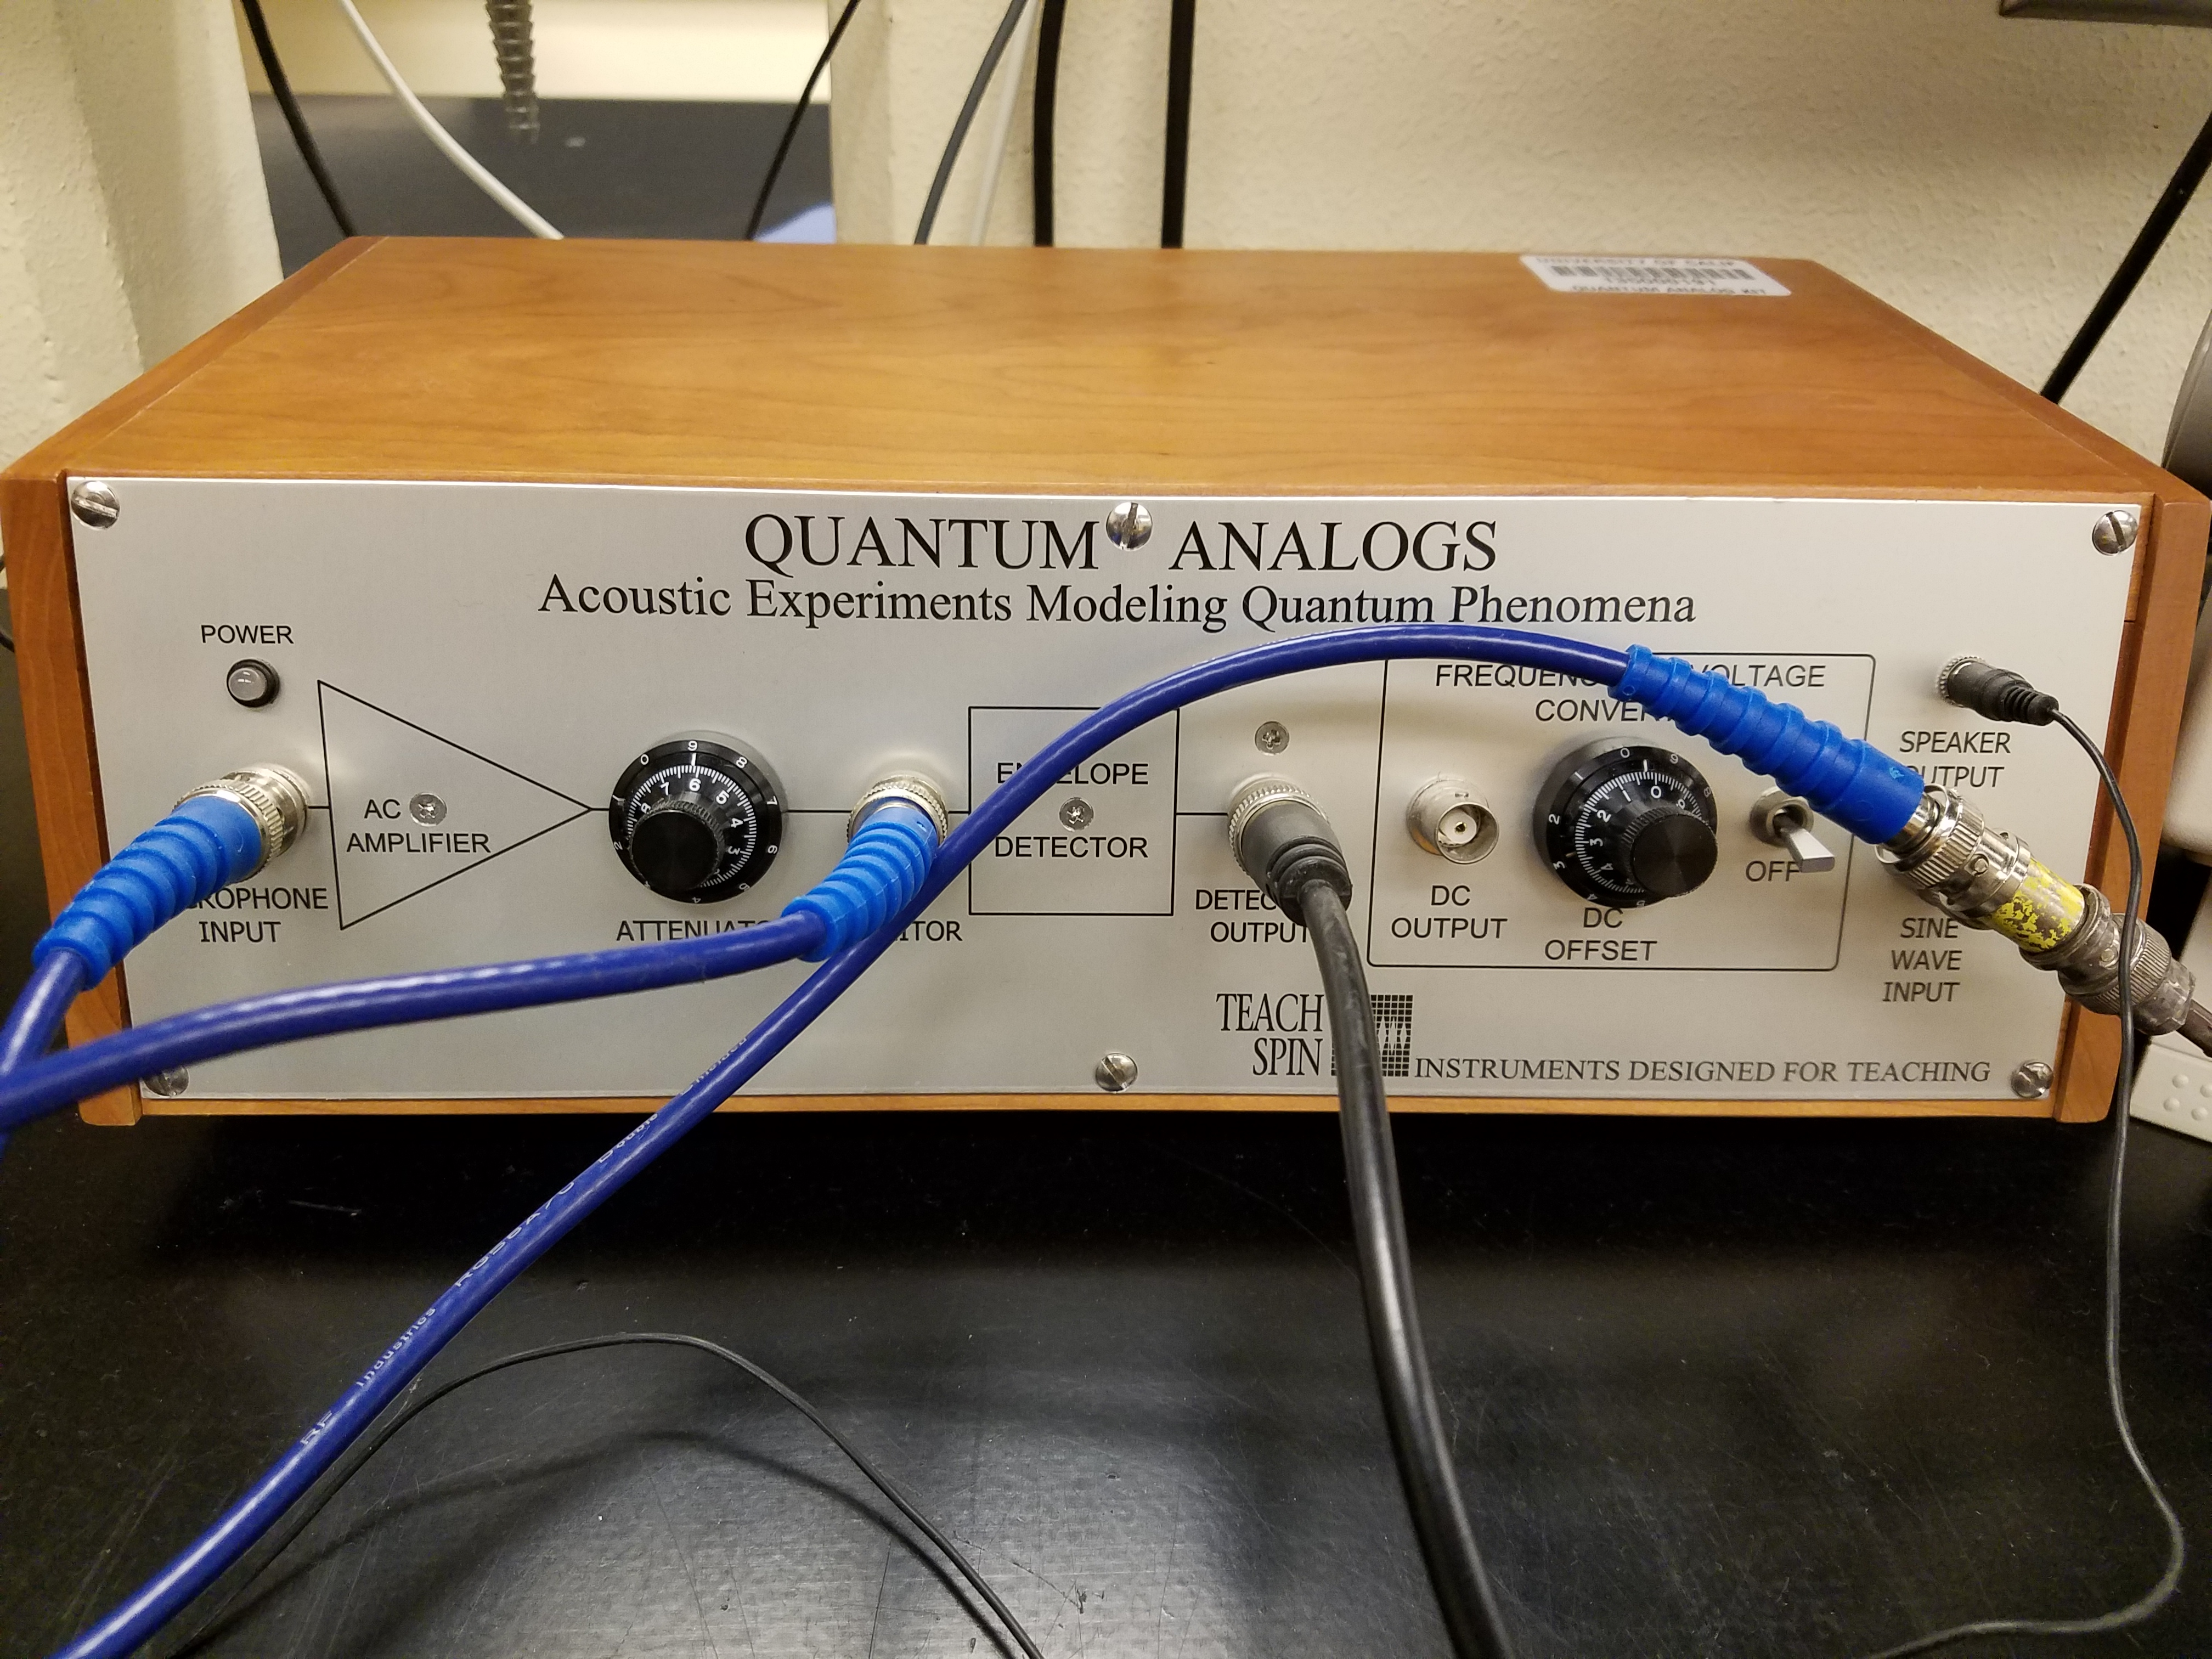
\includegraphics[width=0.4\textwidth]{Setup/AnalogsDevice}\label{QAController}}
		\qquad
		\subfloat[Lab bench]{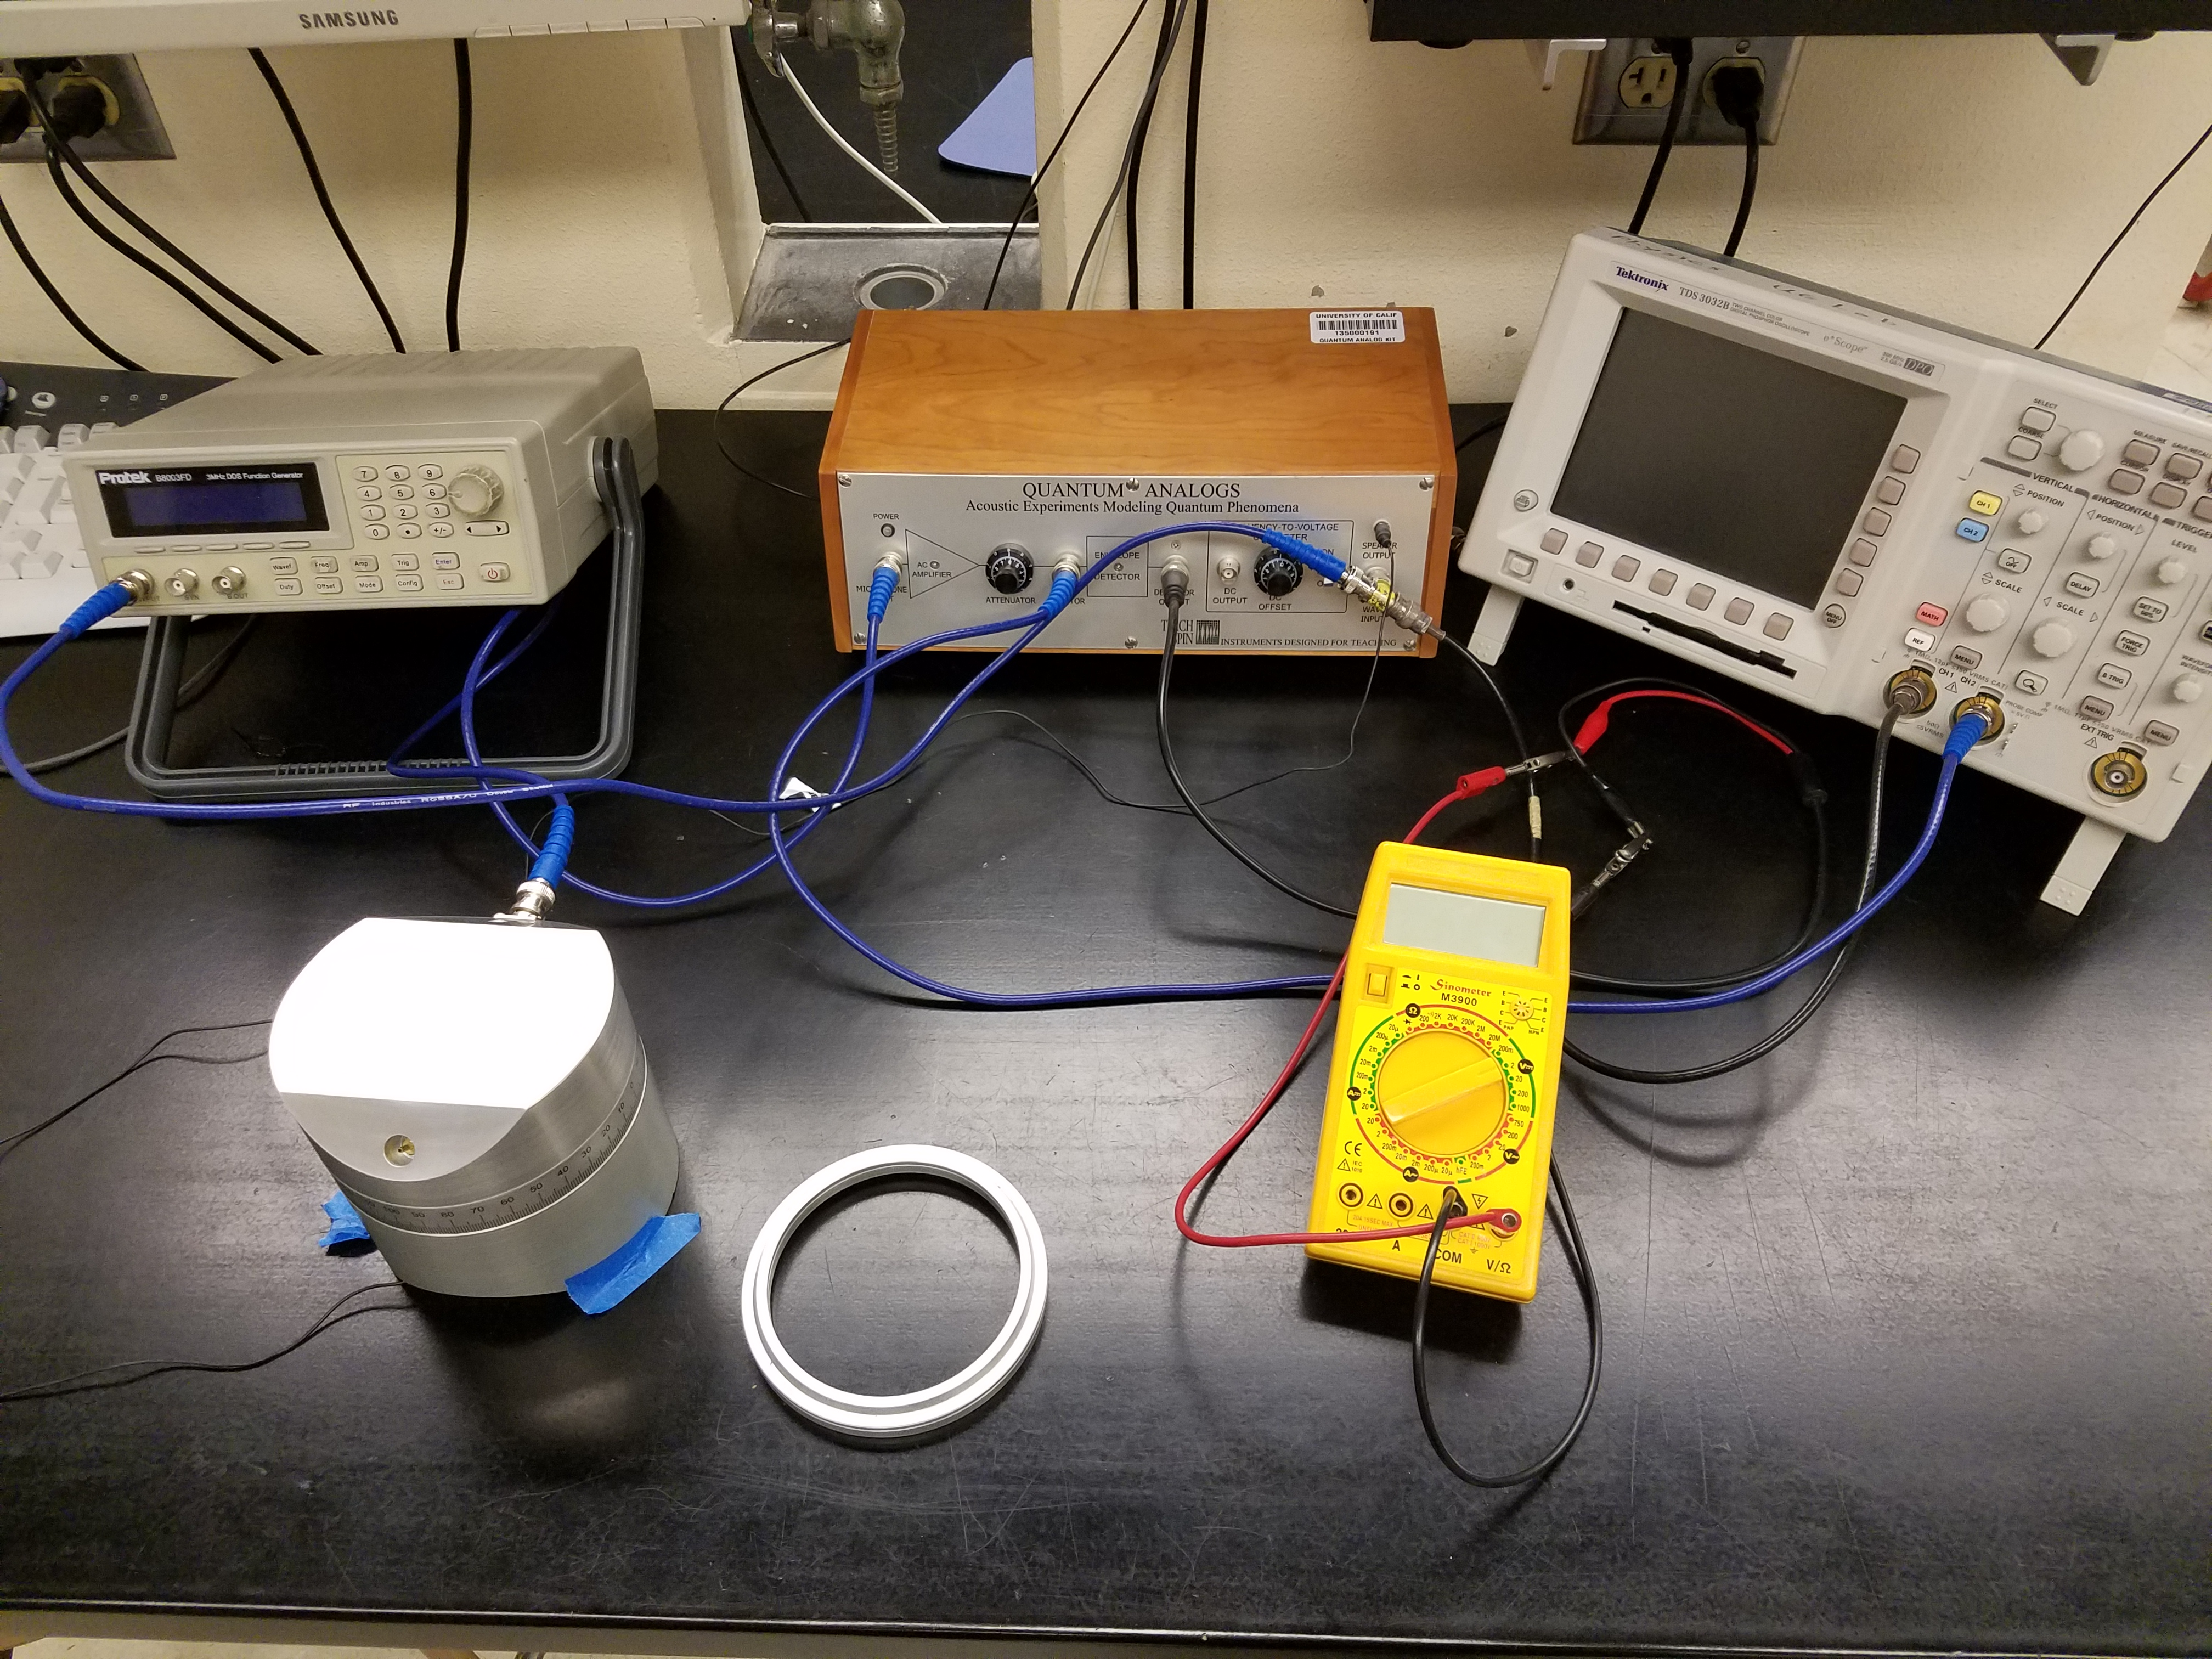
\includegraphics[width=0.4\textwidth]{Setup/Table}
		\label{Setup}}
		\caption{The \emph{Quantum Analogs Controller} \protect\subref{QAController} and our table setup up \protect\subref{Setup}}
		\label{experiment}
	\end{figure}

%		\subsection{Acoustic Resonances of the Spherical Cavity}
	
	\subsection{Frequency Spectrum}
%	Before we begin mapping out resonant frequencies, we need to find the frequency range where the cavity response is linear. We do this because the equations we seek to model are linear. To do this, we set the attenuation to maximum (10), $\alpha = 180 \deg$, and sweep the frequency from $1$ Hz to $\approx 8$ kHz in increments of $10$ Hz. The linear regime of the signal ranges from about $2$ kHz to $8$ kHz and is seen in \cref{LinRegime}. We use $10$ Hz increments simply to find the neighborhood of a resonance, as greater resolution is not required. After we found the linear regime, we lowered the attenuation to half (5.0) and obtained the spectrum of frequencies with clear resonances, see \cref{Raw50a180}. The two smaller peaks at $\approx 6.5$ kHz and $8$ kHz are products of cross talk, and thus not resonances.
	
	Since the equations we are modeling are linear differential equations, we need to determine the frequency range where the cavity response is linear. We measure the frequency spectrum over the entire frequency range, with the attenuation on the Quantum Analogs device set to its maximum setting, and focus our attention to the region where the spectrum increases linearly. This linear regime of frequency response is between $2$ kHz to $8.1$ kHz and is shown in \cref{LinRegime}. Once we determine the linear regime of the signal, we fine tune the attenuation and speaker amplitude to maximize signal and minimize cross-talk. The frequency spectrum for $\alpha = 180\deg$ and $50\%$ attenuation can be seen in \cref{Raw50a180}. The two smaller peaks at $\approx 6.5$ kHz and $8$ kHz are products of cross talk, and thus not resonances.
	
	\begin{figure}[H]
		\captionsetup{justification = justified}
		\centering
		\subfloat[Linear regime frequency spectrum with maximum attenuation]
		{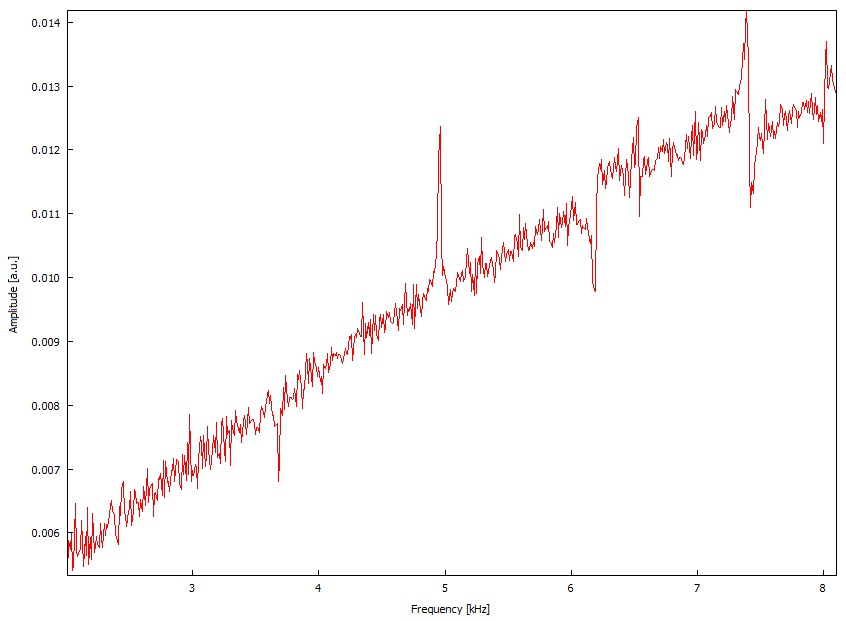
\includegraphics[width=0.4\textwidth]{2.3.2/Raw100a180.jpg}
			\label{LinRegime}}
		\qquad \quad
		\subfloat[Linear regime frequency spectrum with half attenuated signal]{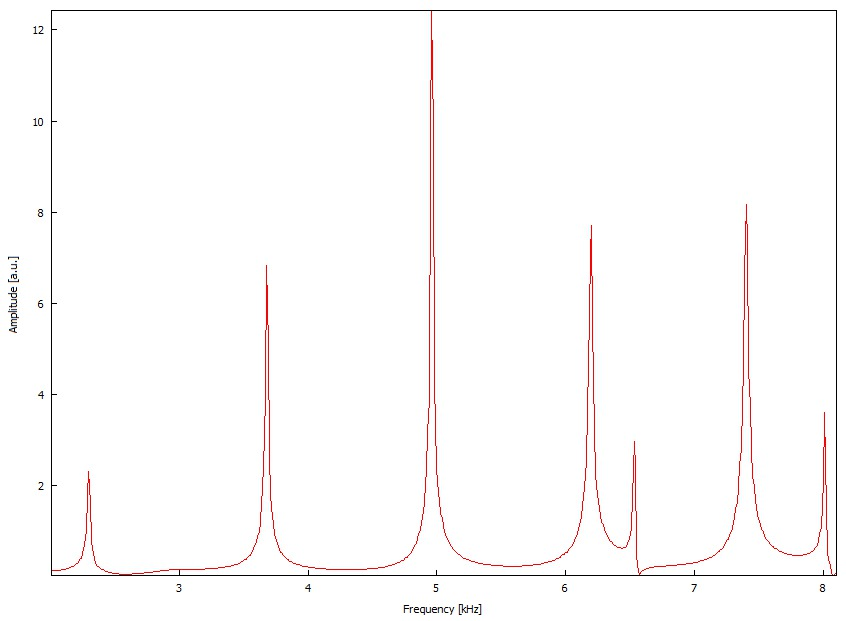
\includegraphics[width=0.4\textwidth]{2.3.2/Raw50a180.jpg}
			\label{Raw50a180}}
		\caption{Fig \protect\subref{LinRegime} shows the linear regime of the frequency spectrum with maximum attenuation. Fig \protect\subref{Raw50a180} shows that same frequency range with a half-attenuated signal.}
		\label{freqSpec}
	\end{figure}
	



	
	\subsection{Measuring Spherical Cavity Resonances with the Computer}
	In this section, we used the sound card in the computer to both generate and measure the resonances within the cavity. We set the attenuator to its highest value ($10$) to protect the sound card. The sound card output is connected to the Quantum Analogs \emph{Sine Wave Input} and to channel 1 of the oscilloscope. The \emph{AC Monitor} from the Quantum Analogs device is connected to the microphone input on the sound card and to channel 2 of the oscilloscope. 
	

	
%	Starting with $\alpha = 180 \deg$ and a step size of $10$ Hz, we sweep from $2$ to $8.1$ kHz and record the amplitude. We repeat this process for $\alpha = 40\deg, 20\deg$ and $0\deg$. We resolved the peak around $5$ kHz by decreasing the step size to from $10$ Hz to $0.5$ Hz. \red{figure references} 
	
	\subsection{Potential Problems}
	One potential problem is the phenomena of \emph{cross talk} when taking measurements with the computer. When the computer is being used to take measurements, it is simultaneously supplying the signal into the cavity. Cross talk occurs when the signal being sent into the cavity crosses into the line coming out of the cavity. Hence the input and output channels of the computer ``talk'' to each other. 
	
	One surefire way to eliminate cross talk is to simply use a higher quality sound card. If this is not an option, you will need to resort to adjusting the amplitude of the output, attenuation, and microphone sensitivities to minimize cross talk.
	
	
	
	
\section{Results and Analysis}
	
	\subsection{Determining Resonant Frequencies}
	Once we restricted our attention to the linear regime, see \cref{Raw50a180}, we began isolating the resonant frequencies using the oscilloscope.
	
	On the oscilloscope, a resonance will appear as a sharp spike with amplitude about 5 or 6 times larger than the characteristic signal amplitude. Near a resonance, we fine tune the frequency in increments of $1$ Hz until the amplitude is maximized. It is important to note that denominations smaller than $1$ Hz are not discernible on the oscilloscope due to the limited resolution of the screen. A table summarizing the resonant frequencies and their nodal angles is provided in \cref{freqTable}. For a full summary of the acoustic amplitude vs polar angle measurements for all resonant frequencies, see \cref{2291Table,3679Table,4962Table,6202Table,7409Table} in the appendix. For the corresponding graphs of acoustic pressure versus polar angle, see \cref{2291Graph,3679Graph,4962Graph,6202Graph,7409Graph}.
	
	\begin{table}[H]
		\captionsetup{justification = centering}
		\centering
		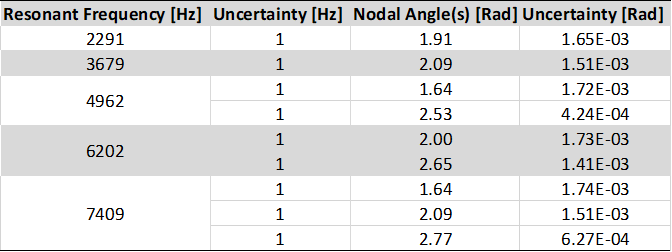
\includegraphics[width=0.6\textwidth]{Tables/ResTable.png}
		\caption{Table of measured resonant frequencies, nodal angles, and associated uncertainties.}
		\label{freqTable}
	\end{table}

	\subsection{Spectrum Response to Varying $\alpha$}
	Once we obtained the frequency spectrum in the linear regime of the signal, we varied $\alpha$ to observe how the spectrum changes as a function of cavity angle. Below are a series of measurements which show how the spectra changes as the cavity angle decreases from $40\deg$ to $0\deg$.
	
	\begin{figure}[H]
		\centering
		\subfloat[Spectrum for $\alpha = 40\deg$]{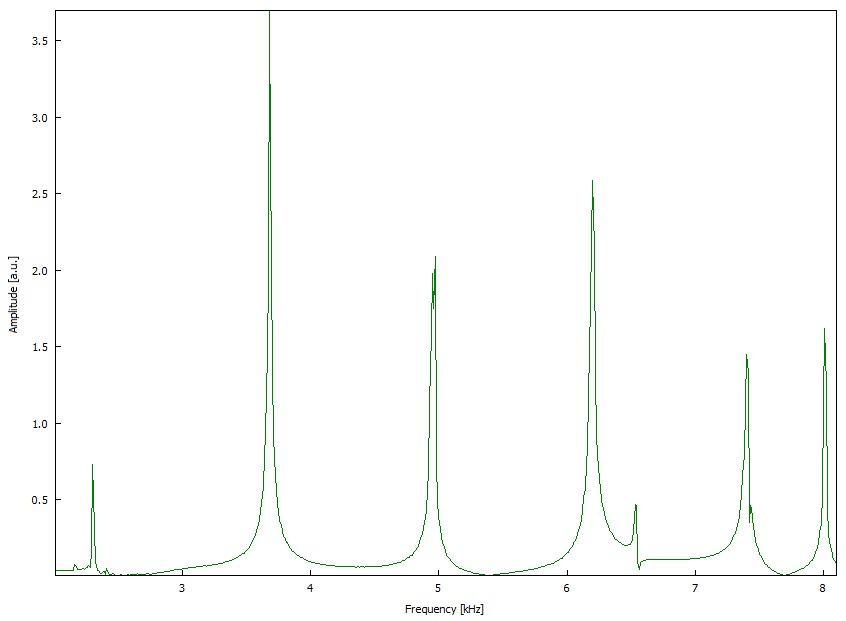
\includegraphics[width=0.3\textwidth ]{2.3.2/Raw50a40.jpg}}
		\quad
		\subfloat[Spectrum for $\alpha = 20\deg$]{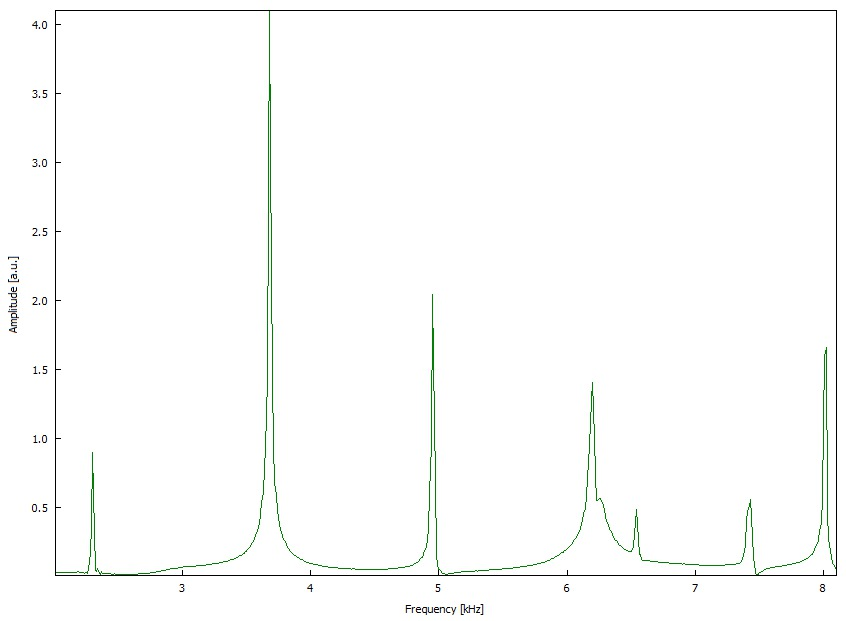
\includegraphics[width=0.3\textwidth]{2.3.2/Raw50a20.jpg}}
		\quad
		\subfloat[Spectrum for $\alpha = 0\deg$]{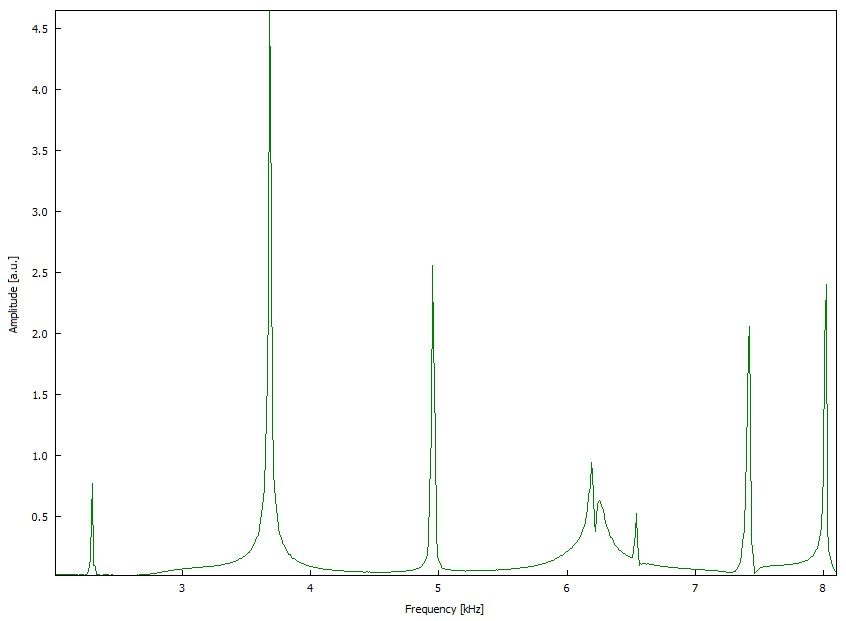
\includegraphics[width=0.3\textwidth]{2.3.2/Raw50a0.jpg}}
		\caption{Graphs showing the spectrum as we vary the cavity angle $\alpha$ from $40\deg$ to $0\deg$. We see very different behavior in the higher frequency resonances.}
		\label{angleSpectra}
	\end{figure}

	From \cref{angleSpectra}, as the cavity angle approaches $0\deg$, the resonance at $\approx6$ kHz starts large and drops off but the resonance at $\approx7.5$ kHz starts large, drops off, and then increases. This is due to the angular dependence of the spherical harmonics and specifically, the Legendre Polynomials. As the order of the polynomial increases, antinodes form closer and closer to $\cos(\theta) = 1$. In other words, the behavior of higher frequency resonances is more erratic near angles close to $\cos(\theta) = 1$, see the Legendre polynomials in \cref{L1,L2,L3,L4,L5} in the appendix. So as we vary the cavity angle from $40\deg$ to $0\deg$, some Legendre polynomials decrease while others increase.


%	\begin{figure}[H]
%		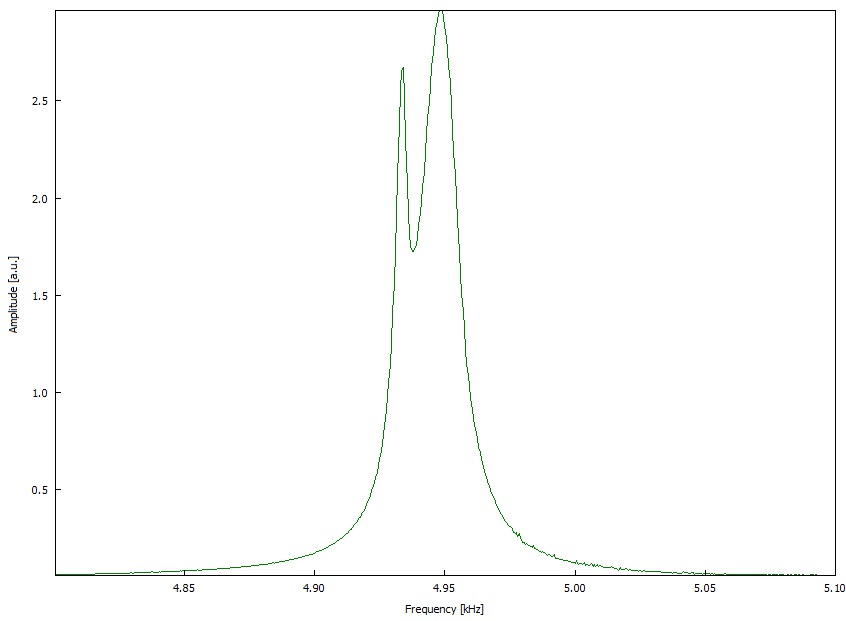
\includegraphics[width=0.3\textwidth]{2.3.2./Raw50a0res.jpg}
%		\caption{Hi resolution spectrum\\ at the $5$ kHz resonance}
%		\label{hiRes5K}
%	\end{figure}
	
		
	
	\subsection{Determining $\ell$ Values for each Resonance}
	Once we isolate the resonant frequencies, their corresponding $\ell$ values can be determined through a qualitative analysis. We will present two ways to achieve this. First, we compare graphs of the acoustic amplitude vs $\cos(\theta)$ to the Legendre polynomials. Since the acoustic amplitude is the analog of the wavefunction, the shape of the graphs should match. Second, we compare the polar plots of acoustic amplitude vs polar angle to the spherical harmonics. This time, the polar plots should match the shapes of the spherical harmonics.
	
	We begin by noting that for any quantum mechanical system, the wavefunction $\psi$ is an inherently imaginary quantity. We can only ever observe real quantities however. To extract any observable quantity from the wavefunction, we must take its amplitude $|\psi|^2$. For the Hydrogen atom, the wavefunction is proportional to the spherical harmonics $\Ylm{\ell}{m}$ and thus also proportional to the Legendre polynomials $\mathrm{P}_\ell(\cos(\theta))$. So, the graphs of acoustic amplitude vs $\cos(\theta)$ should match the magnitude of the Legendre polynomials from the amplitude of the wavefunction $|\mathrm{P}_\ell(\cos(\theta))|^2$. Similarly, polar plots of acoustic amplitude should match the real component of the spherical harmonics.
	

	\subsubsection{Comparison to Legender Polynomials}
	In this section, we determine the $\ell$ value of the $7409$ Hz resonance by comparison to a Legendre polynomial. We present below, a single comparison of acoustic pressure and the corresponding Legendre polynomial. The rest of the comparisons may be found in \cref{legendre1,legendre2,legendre3,legendre4,legendre5} in the Appendix.
	
	\begin{figure}[H]
		\centering
		\subfloat[Amplitude vs $\cos(\theta)$ for the 7409 resonance]{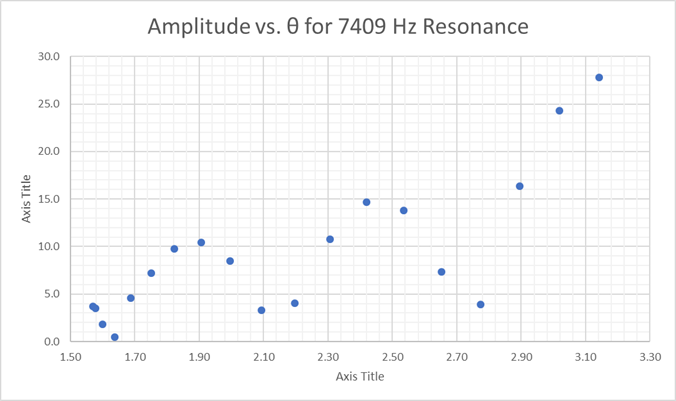
\includegraphics[height=6cm]{Graphs/7409Graph.png}\label{graph1}}
		\qquad
		\subfloat[Legendre polynomial $\mathrm{P}_5(\cos(\theta))$]{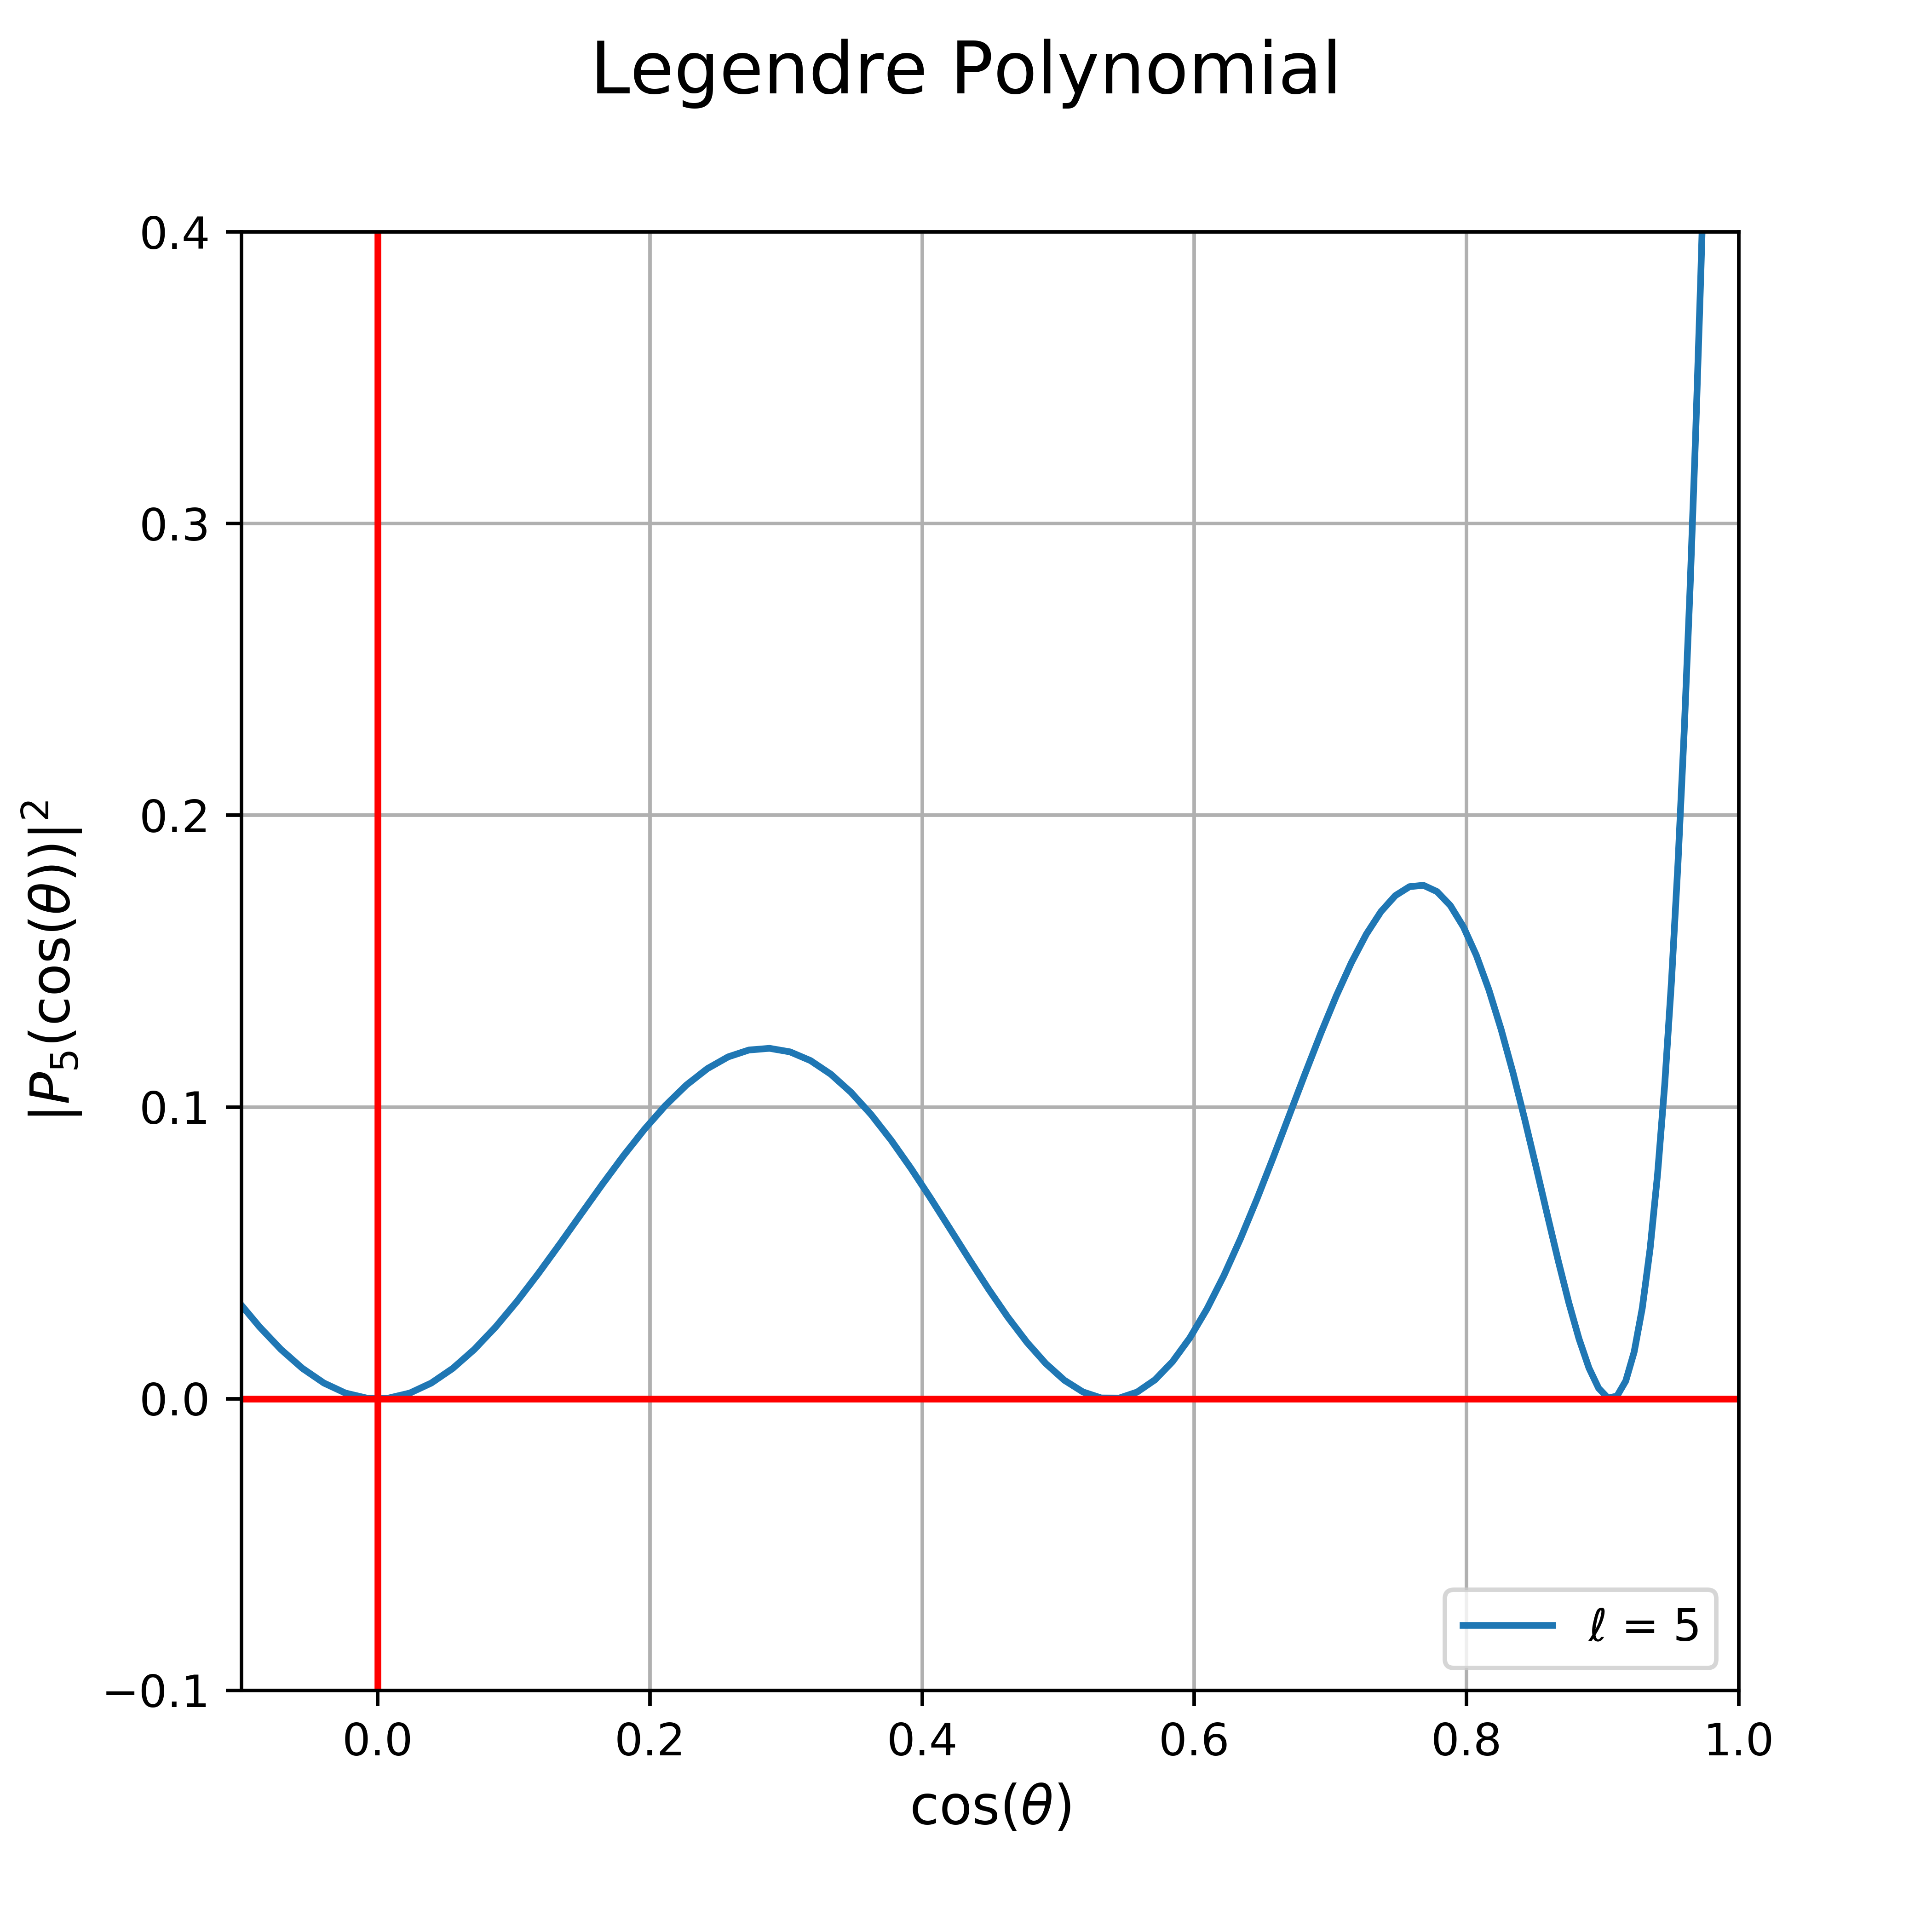
\includegraphics[height=6cm]{Legendre/legendreL5.png}}
		\caption{Qualitative comparison of the 7409 Hz resonance and the $\ell=5$ Legendre polynomial.}
		\label{comparison}
	\end{figure}

	
	The distinguishing features of \cref{graph1} are the starting location at $\cos(\theta) = 0$ and the number of nodes. Since the amplitude starts relatively close to zero, and has $3$ nodes total, a qualitative comparison suggests that the $7409$ Hz resonance corresponds to $\ell=5$.
	
	
	\begin{wraptable}[13]{l}{0.4\textwidth}
		\centering
%		\captionsetup{justification = justified}
		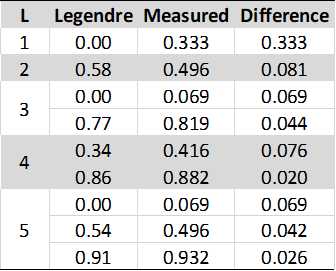
\includegraphics[width=0.3\textwidth]{Tables/LegendreTable.png}
		\caption{Table of numerically calculated zeros of the Legendre polynomials and the measured zeros.}
		\label{legendreTable}
	\end{wraptable}
	

	We may further compare the location of the zeros we measured against the zeros of the Legendre polynomials. I calculated the zeros numerically in Python and summarize the analysis in \cref{legendreTable}. The ``L'' column denotes the $\ell$ value of the Legendre polynomial. The ``Legendre'' column denotes the value of the zero. The column labeled ``Measured'' contains our measured zeros and the ``Difference'' column is simply the difference between the actual value and our measured value.


	\subsubsection{Comparison to Spherical Harmonics}
	To make a comparison to the spherical harmonics, we begin by mapping out how the acoustic amplitude varies as a function of cavity angle at each resonance. We set the angle on the cavity to $\alpha = 180 \deg$ and record the acoustic amplitude using the ``Measure wavefunction'' button on the computer. This process is repeated as $\alpha$ decreases from $180 \deg$ to $0 \deg$ in increments of $\alpha = 10\deg$.
	
	Once we obtain the polar amplitude plots, we may simply compare them to the real component of the spherical harmonics. \cref{SphCompare} below shows one such comparison. The remaining polar acoustic amplitude plots can be seen in \cref{polarGraphs} and their corresponding spherical harmonics in \cref{sphereHarm} in the Appendix. From this qualitative comparison, it is possible to determine the $\ell$ value for each resonance.
	
	\begin{figure}[H]
		\centering
		\subfloat[Acoustic Amplitude vs. polar angle]{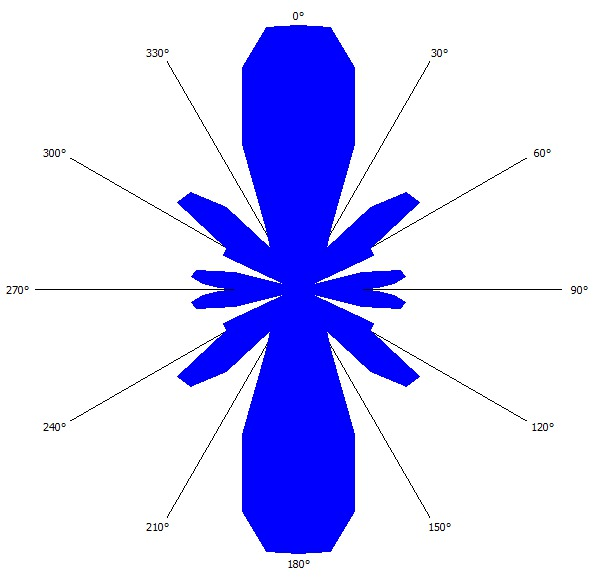
\includegraphics[width=0.3\textwidth]{2.3.2/F7409.jpg}}
		\qquad
		\subfloat[Spherical harmonic corresponding to $\Ylm{0}{5}$]{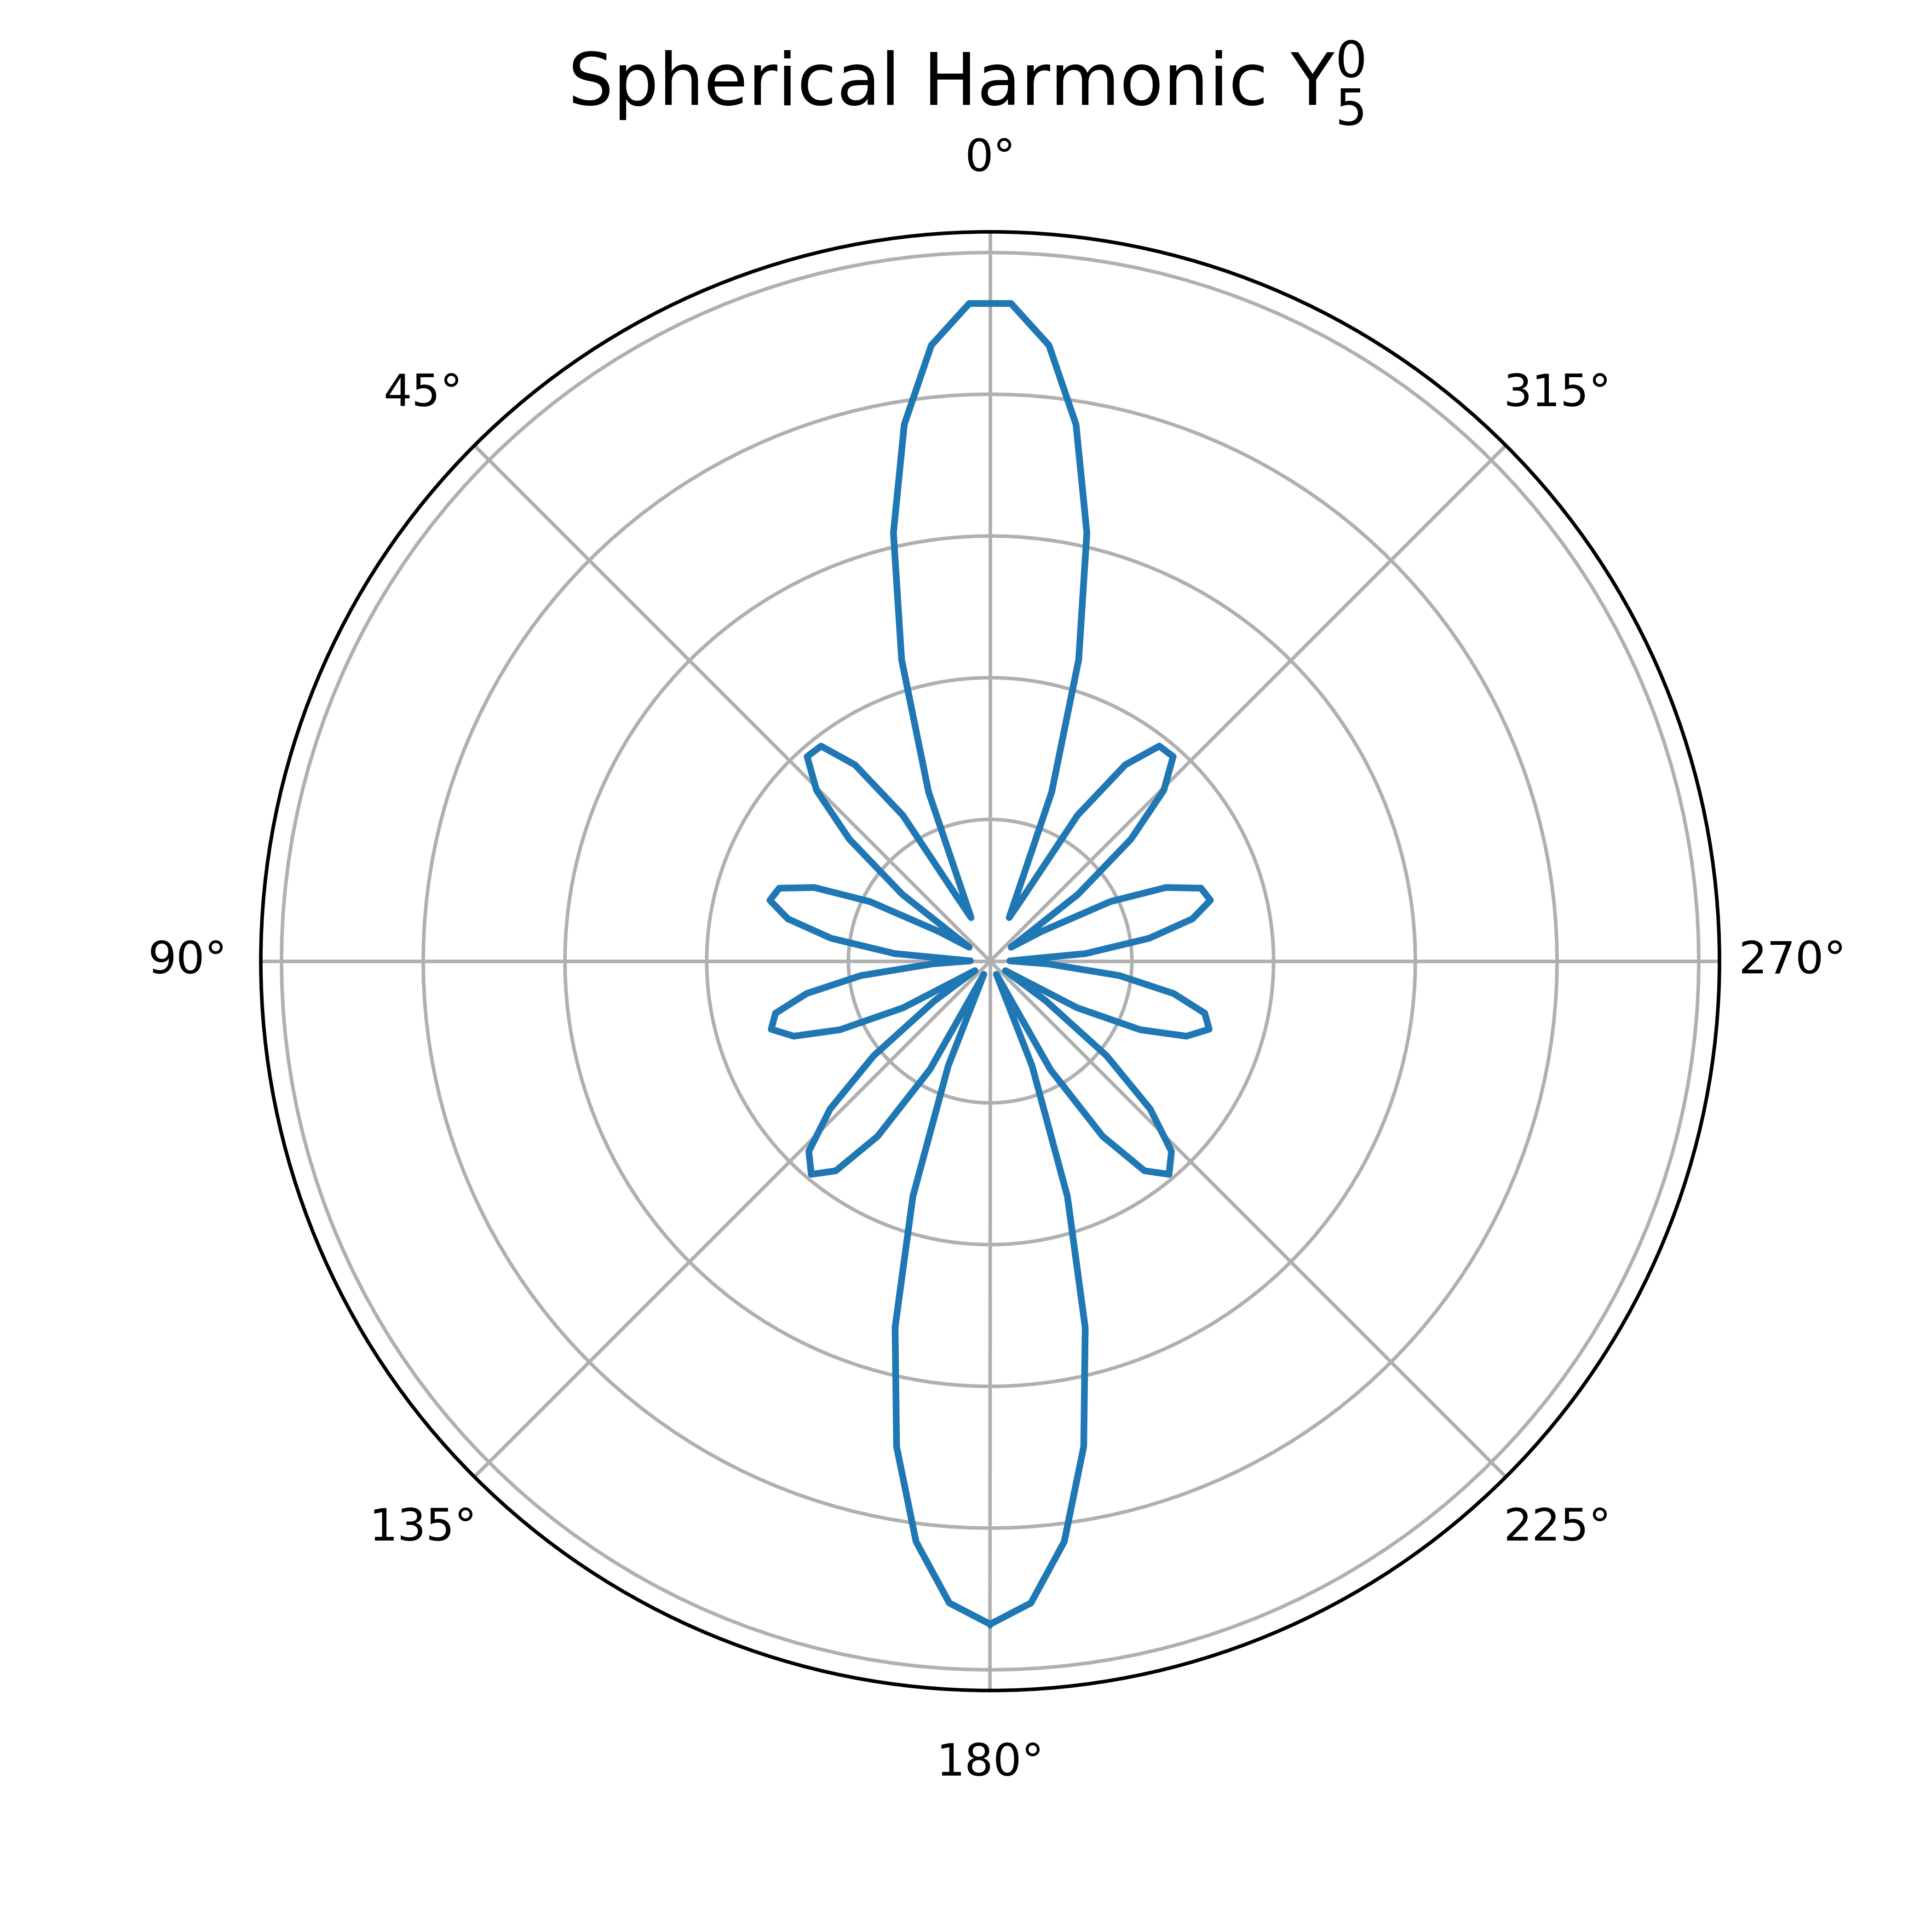
\includegraphics[width=0.3\textwidth]{SphHarm/SphHarmL5M0.png}}
		\caption{A comparison between the acoustic amplitude as a function of cavity angle and the corresponding spherical harmonic for the 7409 Hz resonance.}
		\label{SphCompare}
	\end{figure}
	
	\subsection{$\ell=1$ Degeneracy}
	Recall that a quantum system with angular momentum $\ell$ has a $(2\ell+1)$ degeneracy of states. It is possible to resolve these degeneracies by breaking the spherical symmetry of the cavity. We achieve this by introducing spacing rings into the cavity, simulating a magnetic field which introduces a quantization axis into the system. This symmetry-breaking process is visualized in \cref{degenResolution}, where we can observe the peak splitting as the spacing is increased. The two peaks that emerge are the $m=0$ and $m=\pm1$, which is still degenerate.
	
	\begin{figure}[H]
		\centering
		\subfloat[$\ell=1$ resnonance with spherical symmetry.]{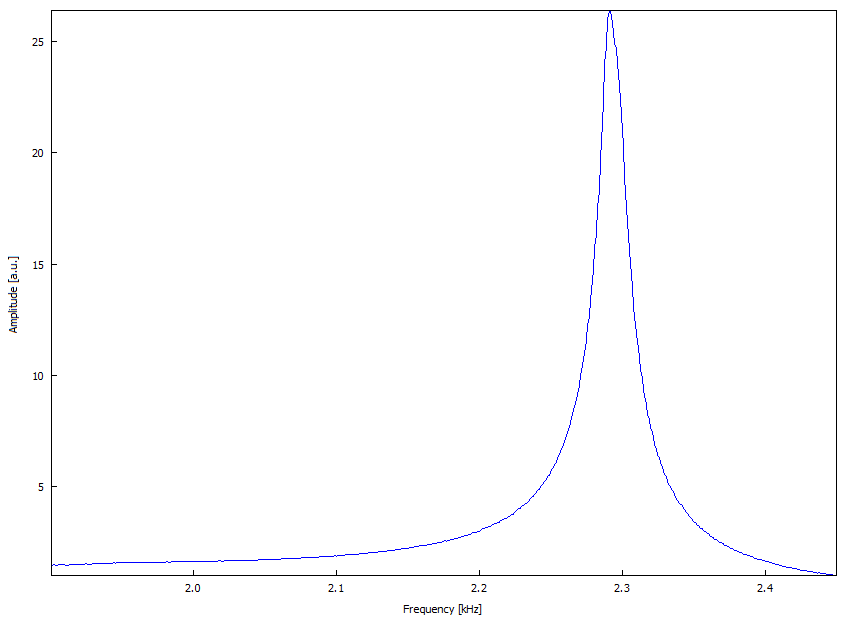
\includegraphics[width=0.3\textwidth]{Day4/L1ResonanceSpectrum.png}\label{degenResolutionSphere}}
		\qquad
		\subfloat[$\ell=1$ resnonance with $3$ mm spacing.]{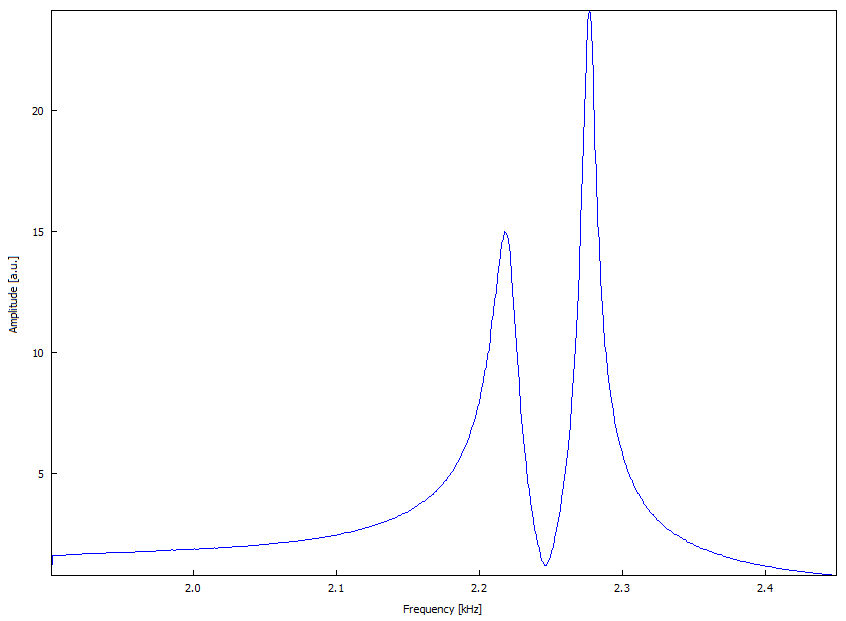
\includegraphics[width=0.3\textwidth]{Day4/L1ResonanceSpectrum3mm.png}\label{degenResolution3mm}}
		\\
		\subfloat[$\ell=1$ resnonance with $6$ mm spacing.]{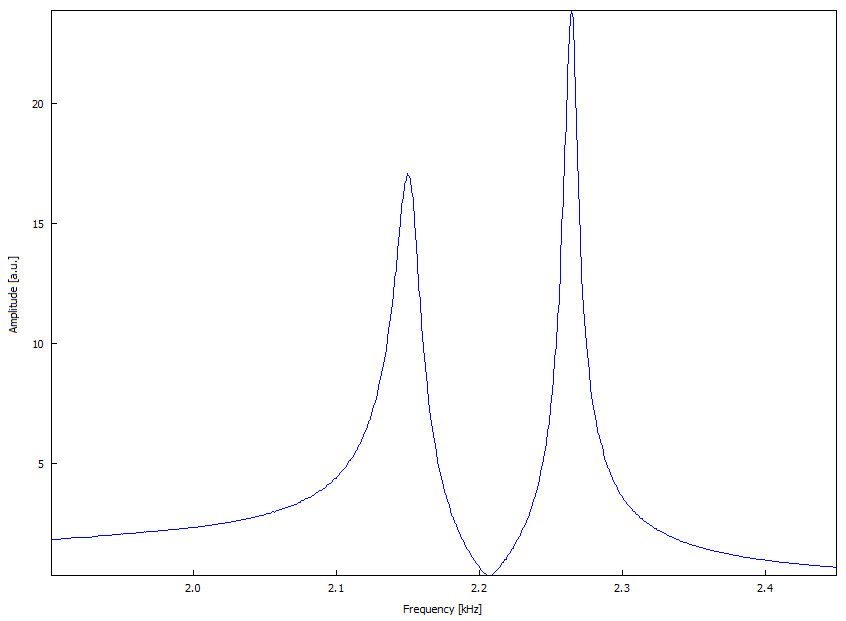
\includegraphics[width=0.3\textwidth]{Day4/L1ResonanceSpectrum6mm.png}\label{degenResolution6mm}}
		\qquad
		\subfloat[$\ell=1$ resnonance with $9$ mm spacing]{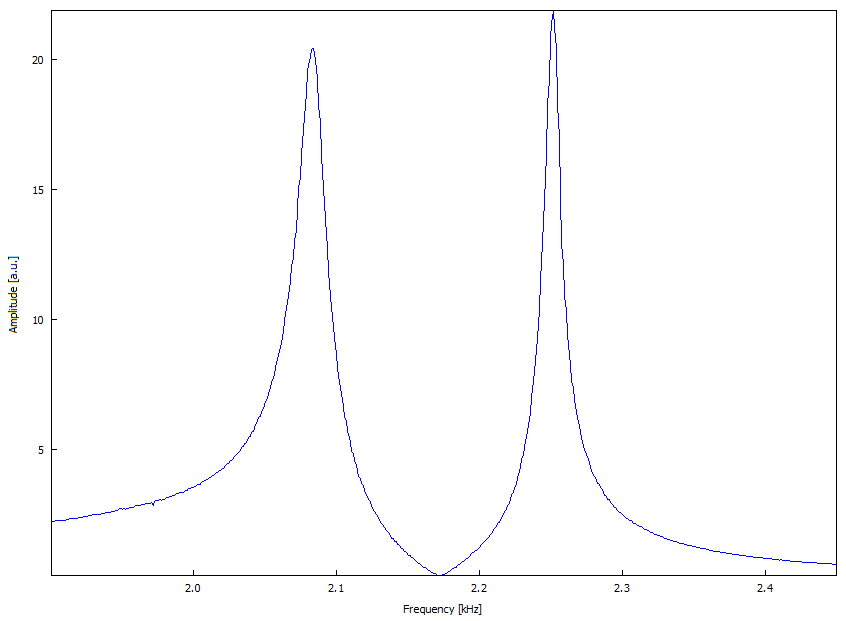
\includegraphics[width=0.3\textwidth]{Day4/L1ResonanceSpectrum9mm.png}\label{degenResolution9mm}}
		\caption{We can see as we break the spherical symmetry by introducing spacer rings to the cavity, the degeneracy in the $\ell=1$ resonance is lifted and we can resolve the $m = 0$ and $m = \pm1$ peaks.}
		\label{degenResolution}
	\end{figure}

	We may further investigate by examining polar plots of the amplitude to determine the magnetic quantum number $m$. \cref{9mmPolarliftedDegeneracy} shows the $\theta = 0$ projection of acoustic pressure vs. azimuthal angle $\varphi$ for a cavity with the maximal separation of $9$ mm. Azimuthal amplitude graphs for the $3$ mm and $6$ mm spacing rings can be seen in \cref{3mmliftedDegeneracy} and \cref{6mmliftedDegeneracy} in the appendix.
	
	\begin{figure}[H]
		\centering
		\subfloat[$\ell=1$, $m=0$ orbital with 9mm spacing.]{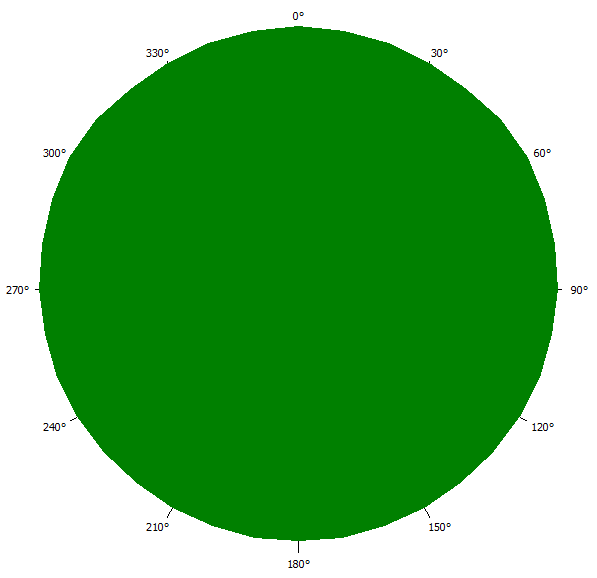
\includegraphics[width=0.3\textwidth]{Day4/L19mmPolar2084_806.png}\label{liftedDegeneracyL1M0}}
		\qquad
		\subfloat[$\ell=1$, $m=\pm1$ orbital with 9mm spacing.]{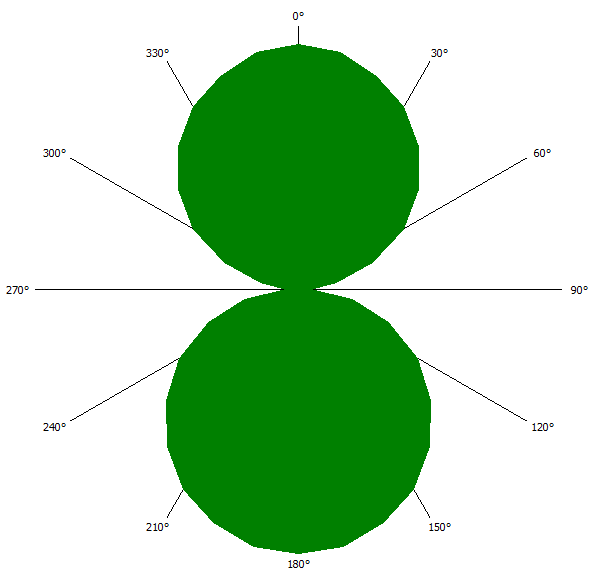
\includegraphics[width=0.3\textwidth]{Day4/L19mmPolar2251_140.png}\label{liftedDegeneracyL1M1}}			
		\caption{Projections of acoustic amplitude vs azimuthal angle $(\varphi)$ onto the $\theta=0$ plane. Angle markings indicate the azimuthal angle $\varphi$.}
		\label{9mmPolarliftedDegeneracy}		
	\end{figure}

	By comparing these graphs to the spherical harmonics, we can resolve the $\ell=1$ state into $m=0$ and $m=\pm1$. 
	The $m=\pm1$ states are still degenerate because they are symmetric under rotations in the azimuthal angle $\varphi$. This can be seen in the $\varphi=0$ projections of the spherical harmonics in \cref{L1M1Comparison}. The projection of \cref{sphHarml1m0} onto the $\theta = 0$ plane exactly recovers \cref{liftedDegeneracyL1M0}. Similarly, the projection of \cref{sphHarml1m1} onto the $\theta = 0$ plane exactly recovers \cref{liftedDegeneracyL1M1} up to rotations in $\phi$

	\begin{figure}[H]
		\centering
		\subfloat[Projection of $\Ylm{1}{0}$ onto the $\varphi = 0$ plane.]{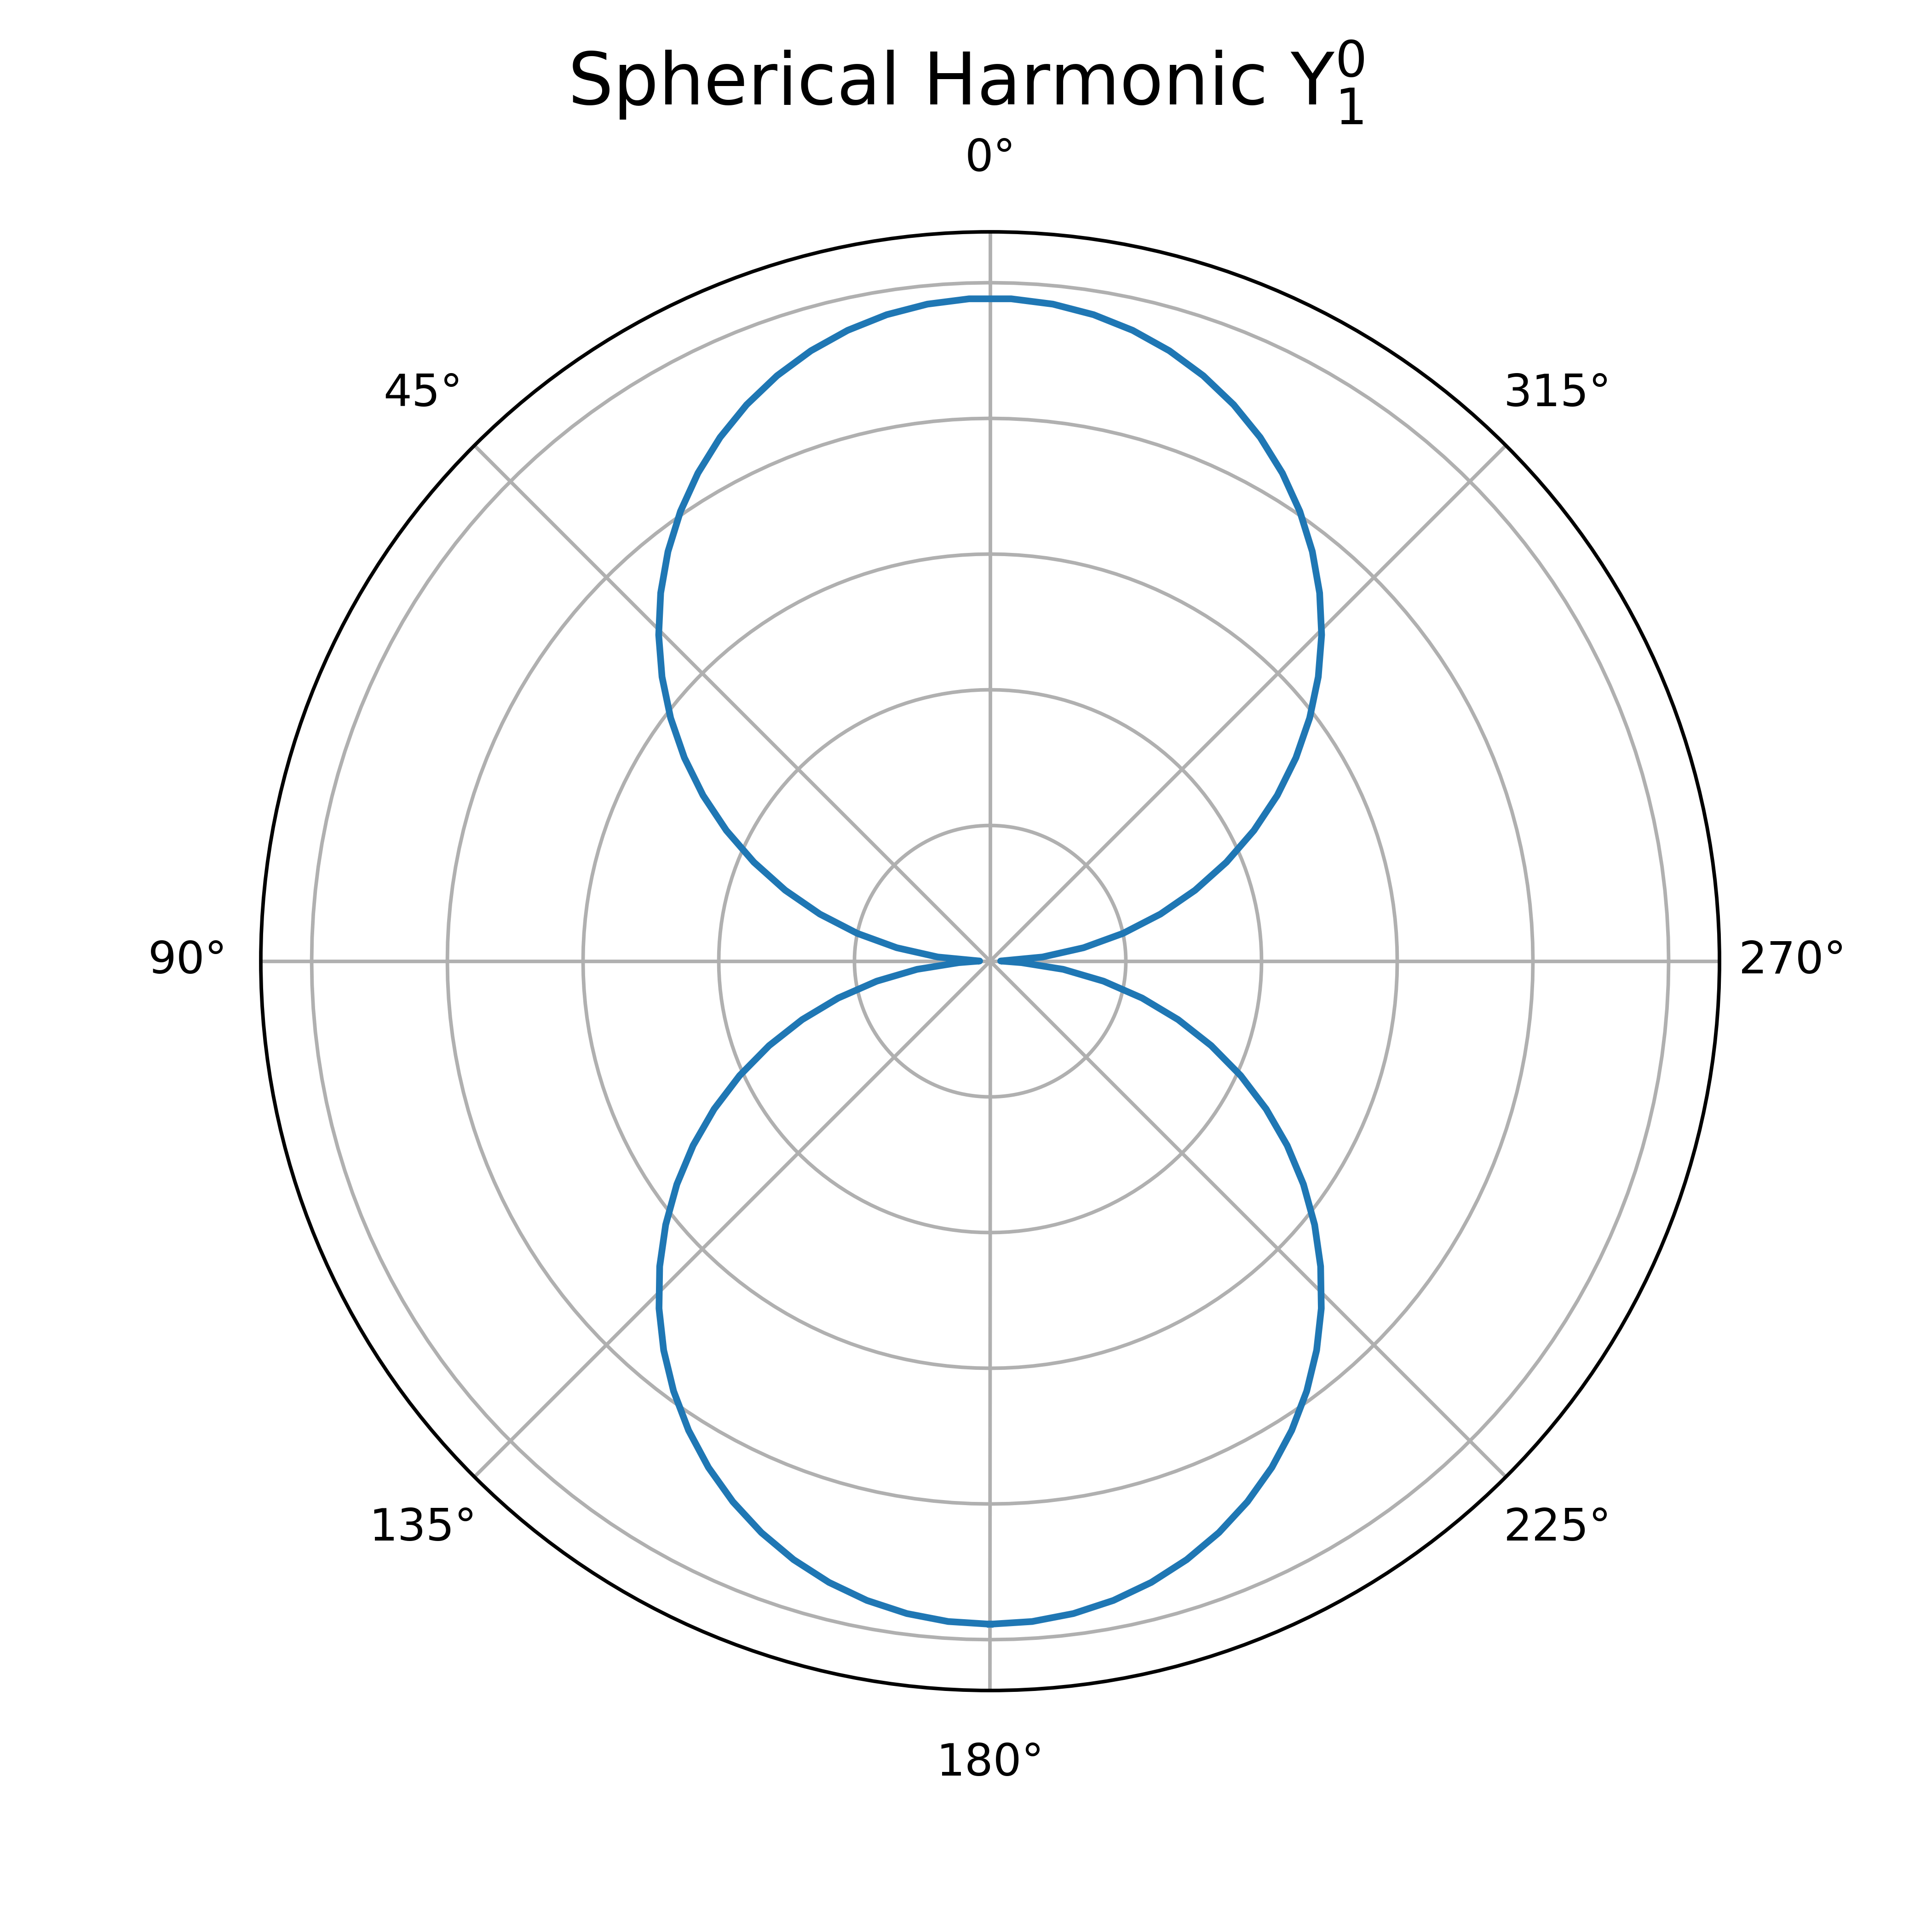
\includegraphics[width=0.35\textwidth]{SphHarm/SphHarmL1M0.png}\label{sphHarml1m0}}
		\qquad
		\subfloat[Projection of $\Ylm{1}{1}$ onto the $\varphi = 0$ plane.]{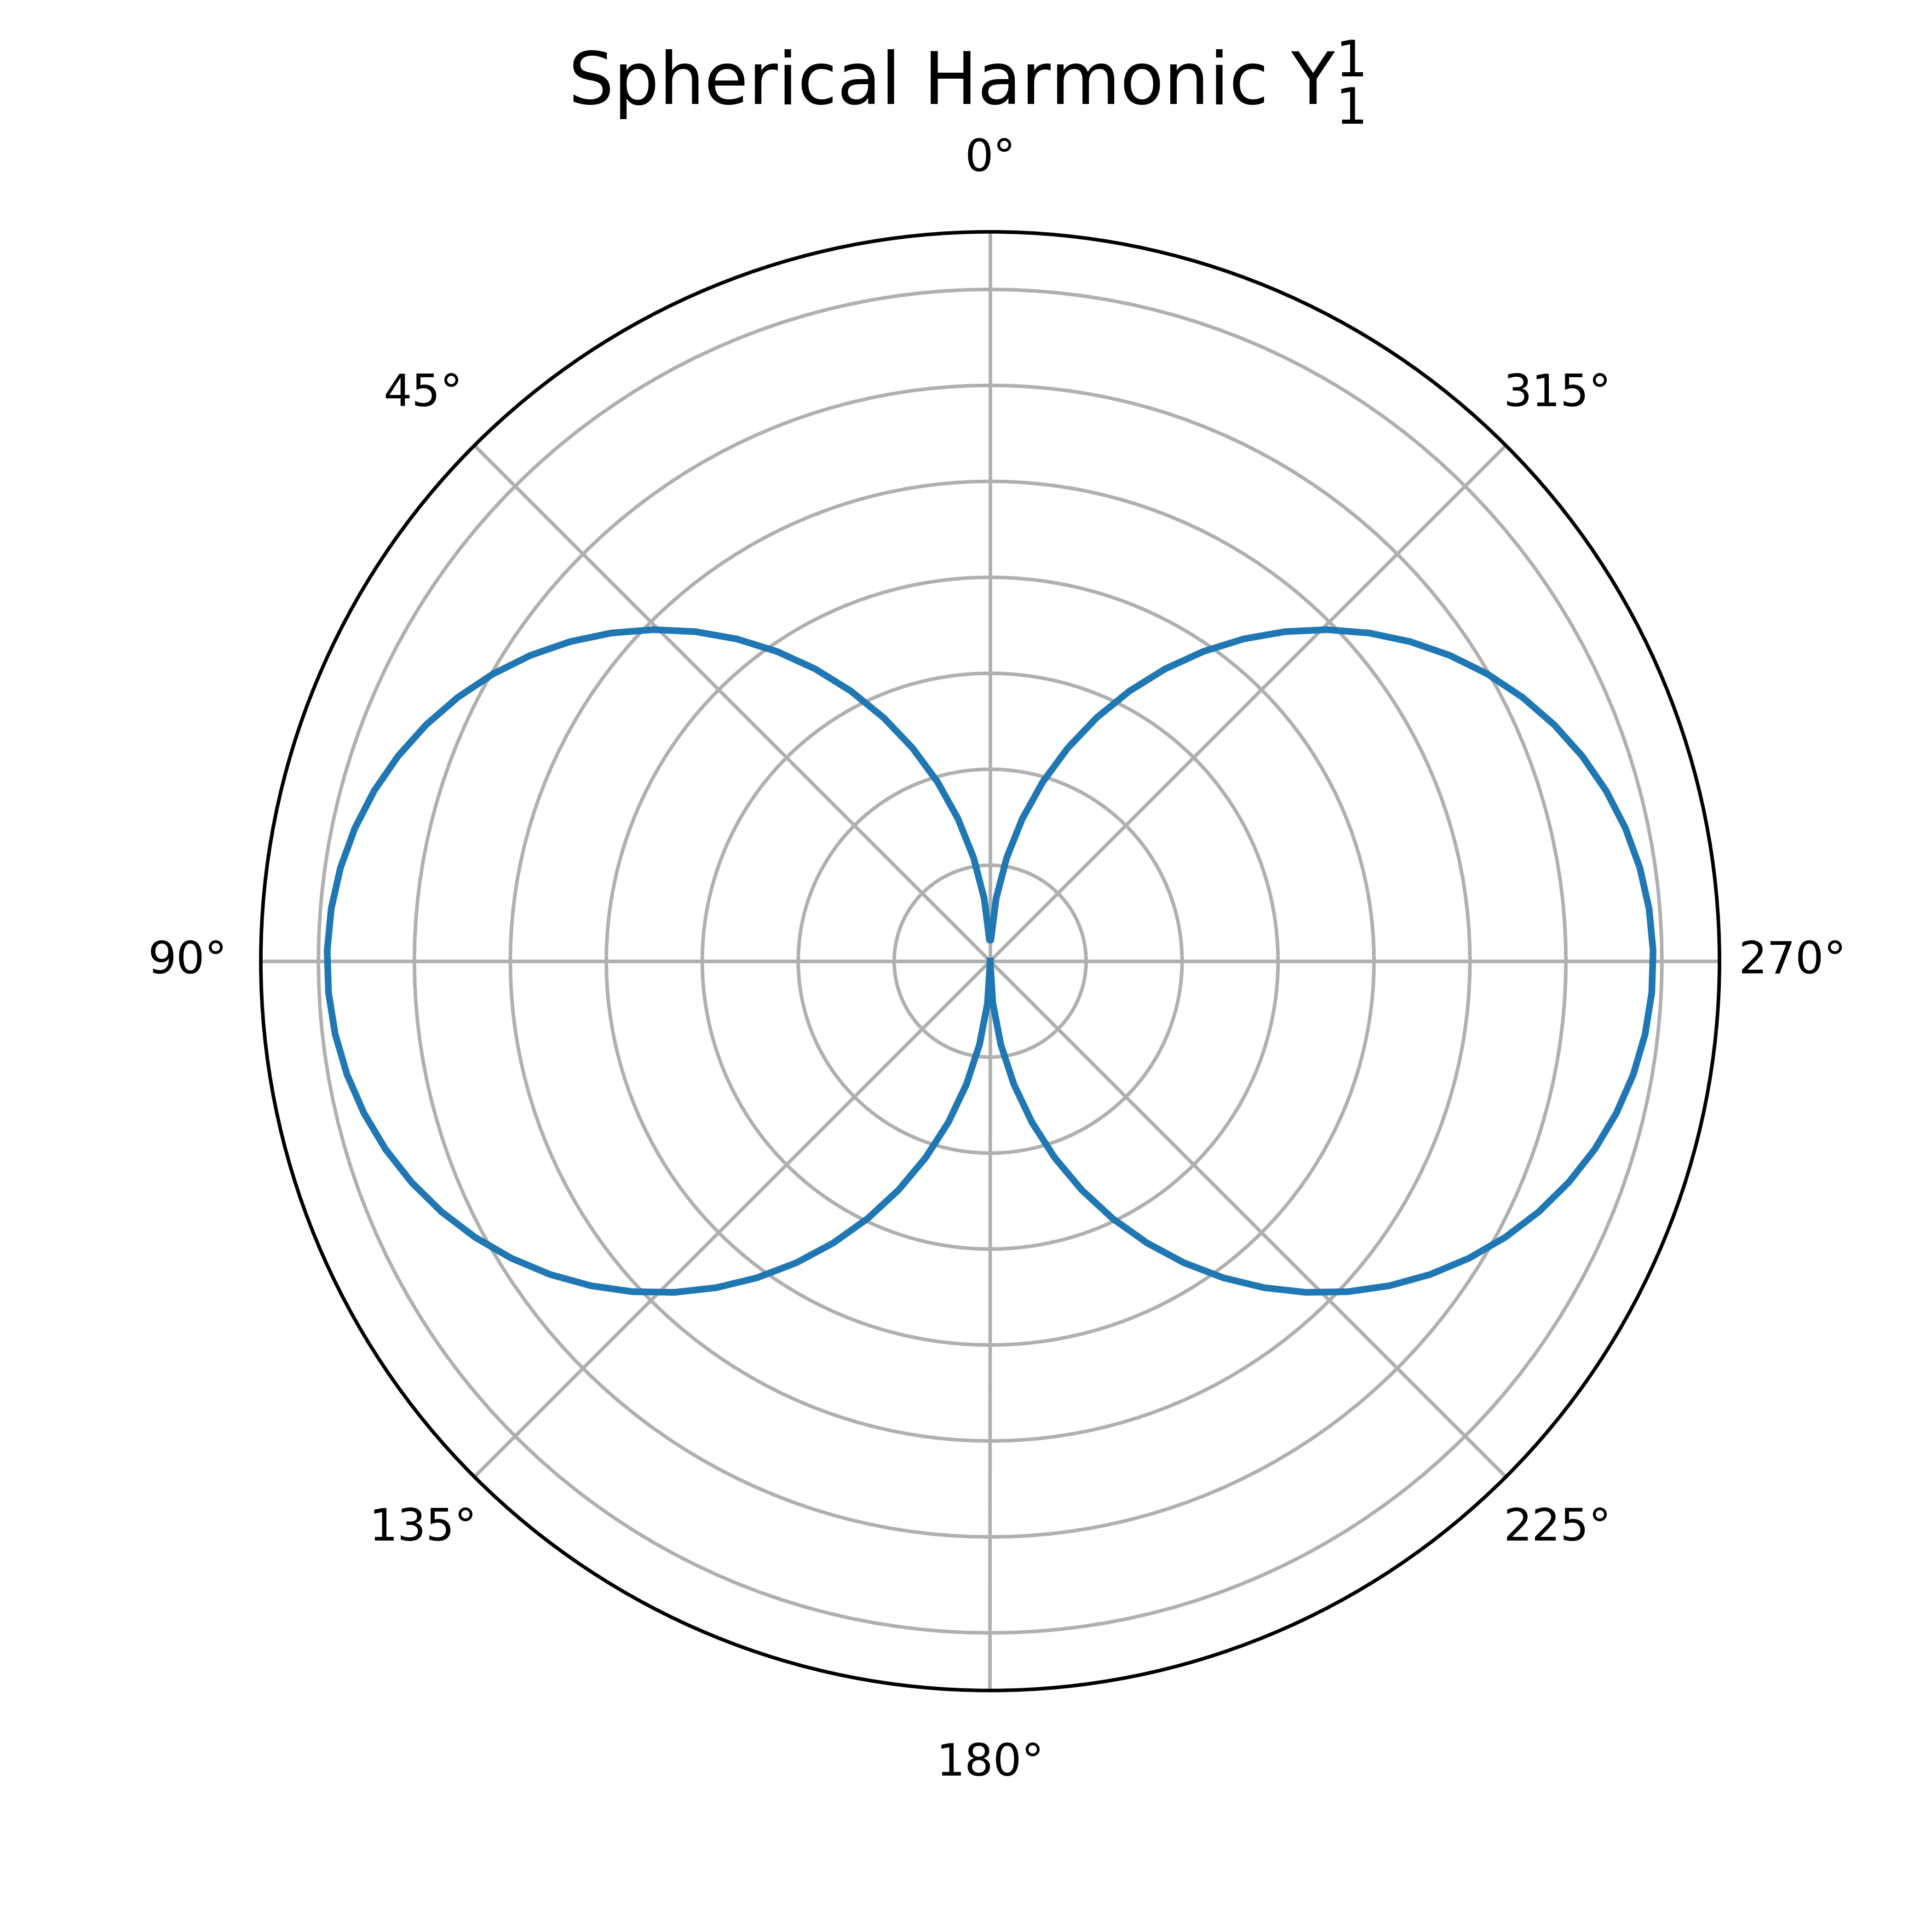
\includegraphics[width=0.35\textwidth]{SphHarm/SphHarmL1M1.png}\label{sphHarml1m1}}
		\caption{Projections of the spherical harmonics onto the $\varphi=0$ plane. Angle markings indicate polar angle $\theta$.}
		\label{L1M1Comparison}
	\end{figure}




\subsection{Phase Measurements}
Upon breaking the spherical symmetry of the cavity, the degeneracy in $\ell=1$ state is partially lifted. One way to see this is to examine the phase of the standing waves. With spherical symmetry, the phase of the standing waves inside the cavity are identical. However, once we break the spherical symmetry, we can begin to see the phases between the $m=0$ and $m=\pm1$ states begin to differ as seen in \cref{phaseTable}. However, because the $m=\pm1$ states are both symmetric in azimuthal, we are unable to resolve their degeneracy

\begin{table}[H]
	\captionsetup{justification = centering}
	\centering
	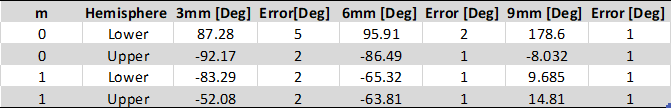
\includegraphics[width=0.8\textwidth]{Tables/PhaseMeasurements.png}
	\caption{Phase measurements for top and bottom hemispheres}
	\label{phaseTable}
\end{table}



\section{Conclusion}

	\subsection{Achievements}
	In this experiment, we successfully modeled the angular dependence of the Hydrogen wavefunction with a standing pressure wave inside a spherical cavity. We are able to identify the $\ell$ values of each resonance by comparison to the Legendre polynomials and the spherical harmonics. Further, we simulated the Zeeman effect, which breaks the spherical symmetry, by introducing spacing rings into the cavity. Because the symmetry is broken, some of the degeneracies in $\ell$ are resolved. We were only able to resolve the $m=0$ and $m=\pm1$ states however because $m=\pm1$ is symmetric in the azimuthal angle.

	\subsection{Future Improvements}
	Throughout this experiment, the microphone was extremely sensitive to any noise and even vibrations in the room, chairs moving, the lab bench being bumped, doors closing, etc... One improvement to this experiment is to perform it in an isolated room on a sand table which dampens vibrations from the environment.
	
	One natural extension to this experiment is to measure the $m$ states for higher resonances. Higher resonances correspond to larger $\ell$ values, which contain $2\ell + 1$ degeneracies. Breaking the spherical symmetry, we should be able to resolve some of the degeneracies. Again, we expect to find that we can only resolve the degeneracies in $m$ up to a sign. 
	
	Finally, one potentially interesting avenue to explore is to change the density of the gas 
	Since the velocity of the standing waves inside the cavity depends on the composition of the gas, one interesting avenue to explore is to change the density of the gas inside the cavity. For gases less dense than air, the standing waves travel faster and the resonant frequencies are expected to increase. 
	
	
	
%Appendix A


\section{Appendix}
\label{AppendixA}

All numerical calculations were written and performed in Python.

\subsection{Cavity Angle and Polar Angle Relation}

\begin{figure}[H]
	\centering
	\captionsetup{justification = raggedright}
	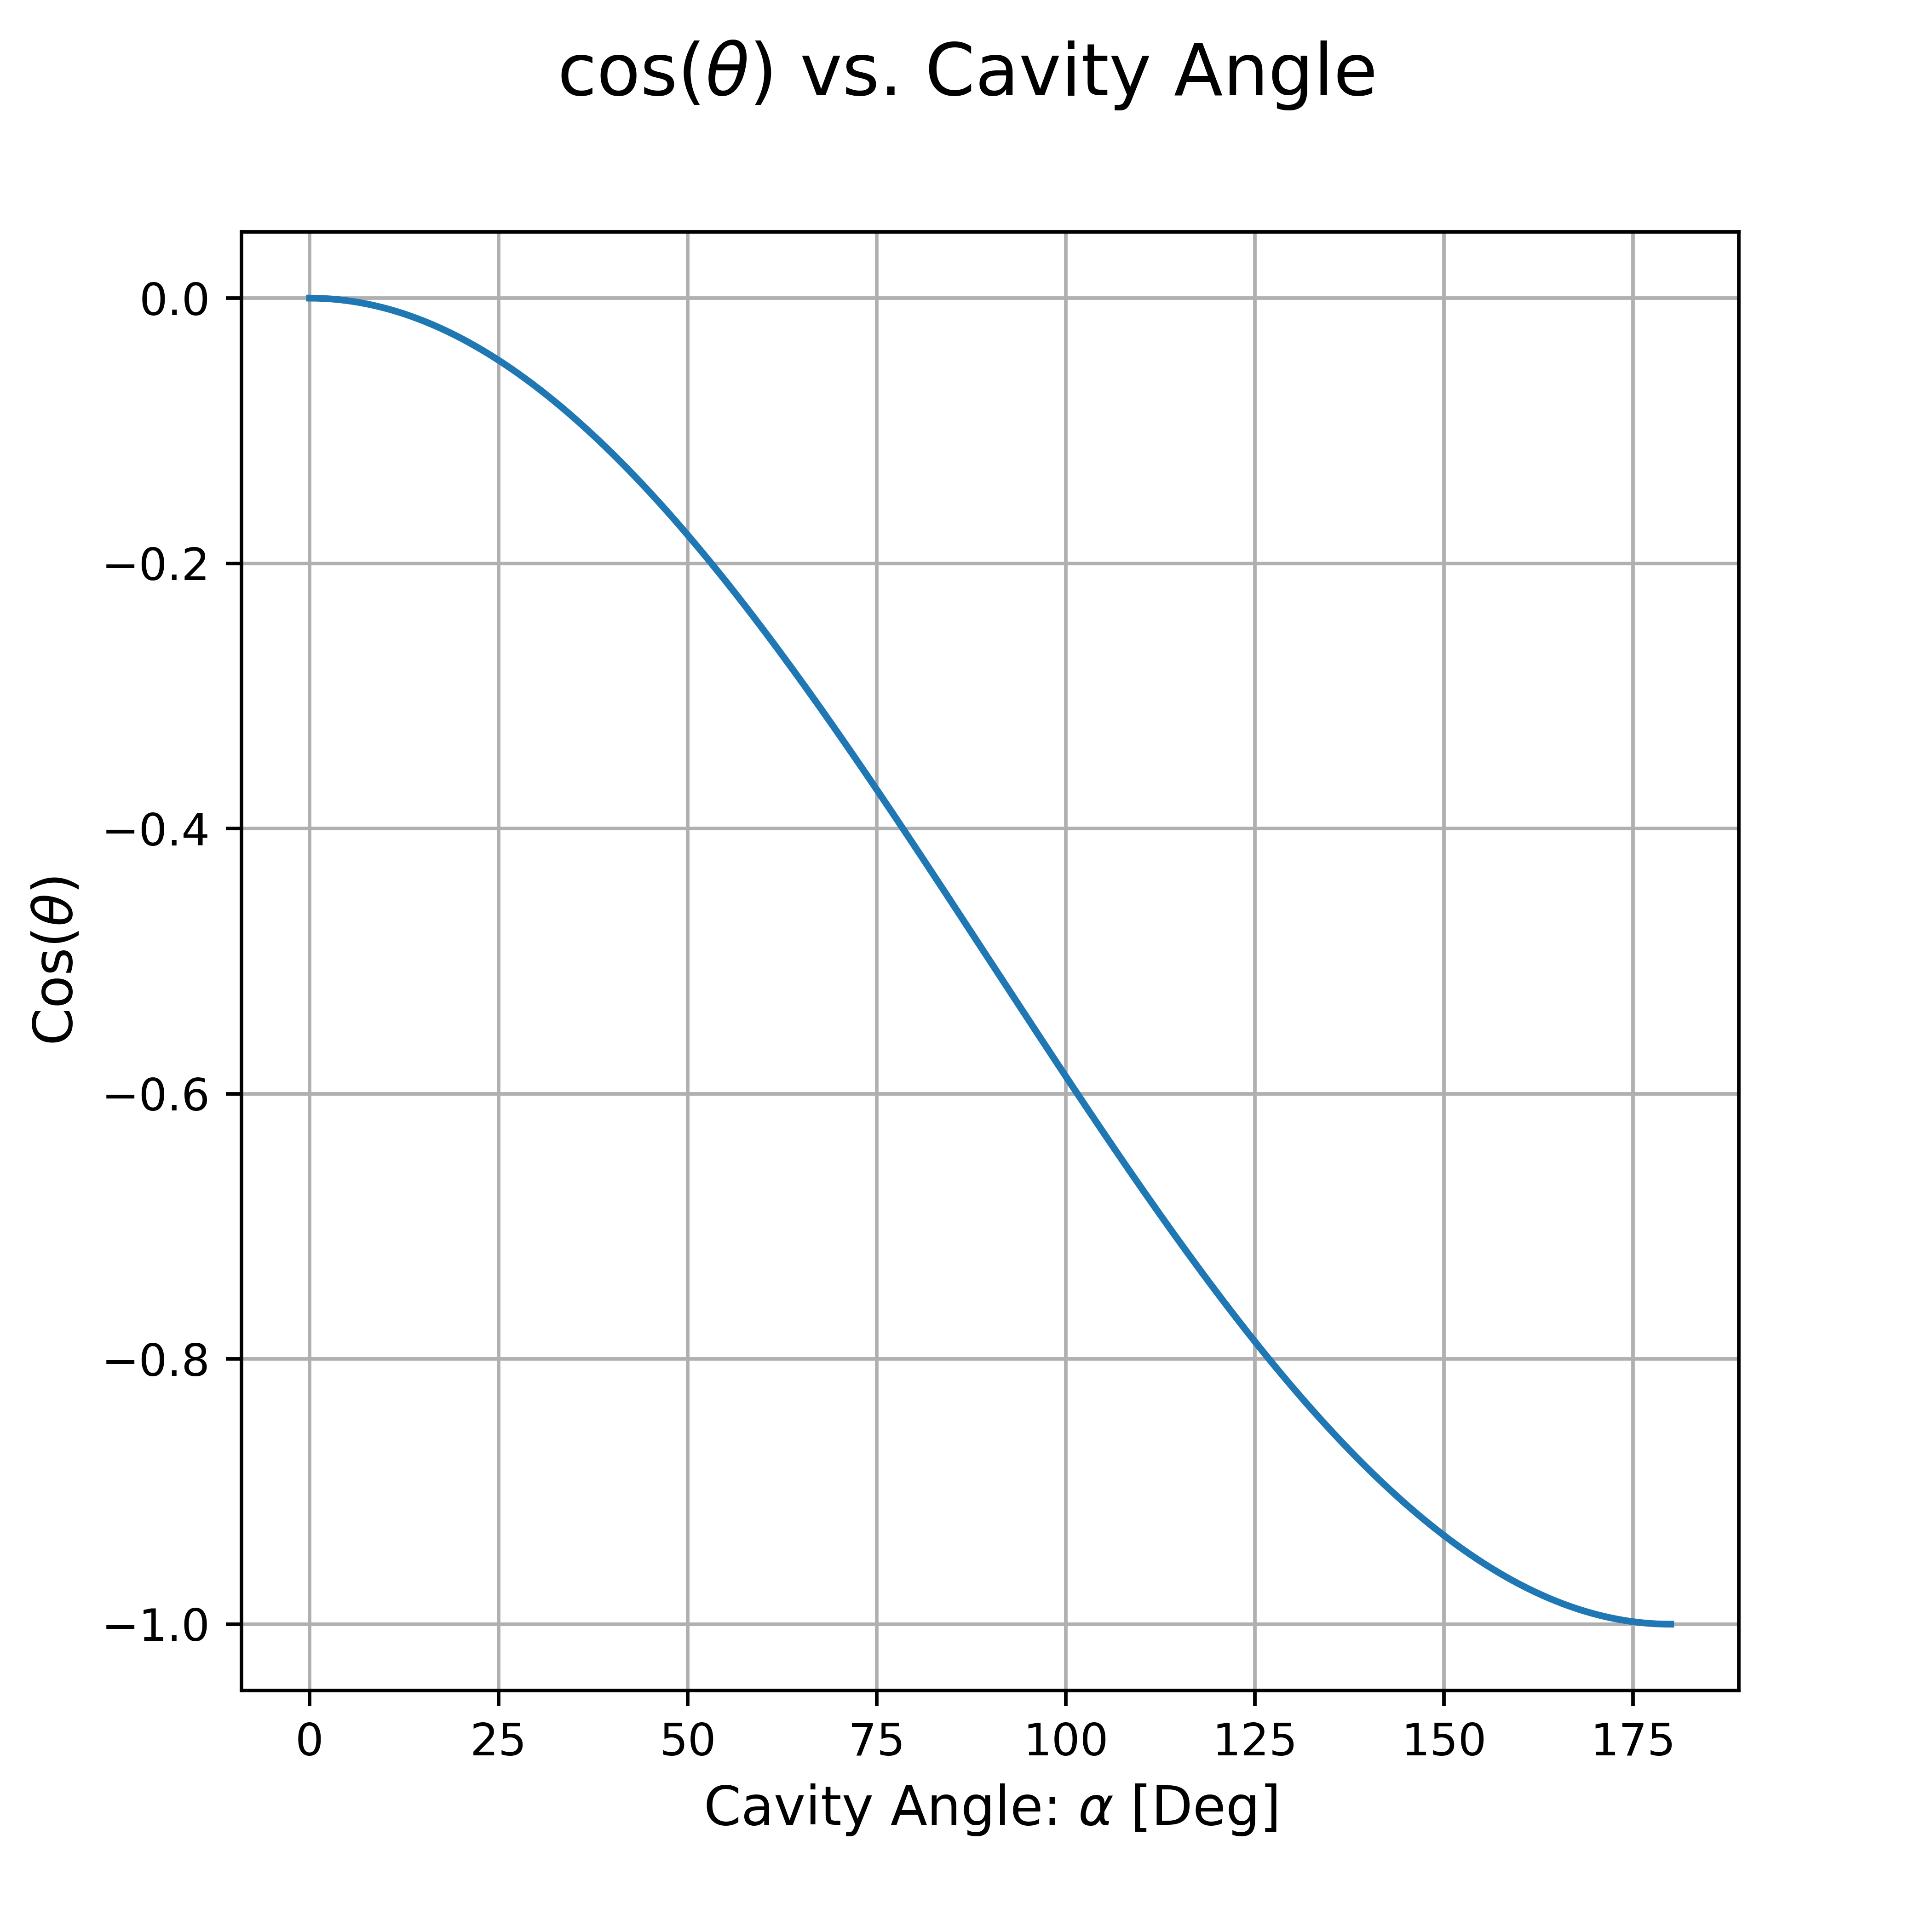
\includegraphics[width=0.4\textwidth]{Graphs/ThetaAlpha.png}
	\caption{Relation between $\cos(\theta)$ and cavity angle $\alpha$ when spherical symmetry is present}
	\label{ThetaAlpha}
\end{figure}


\subsection{Amplitude and Polar Angle Measurement Tables}
For clarity, instead of plotting $\cos(\theta)$ we plot $|\cos(\theta)|$ since cosine is symmetric about $\theta = 0$.

\begin{multicols}{2}
	\begin{table}[H]
		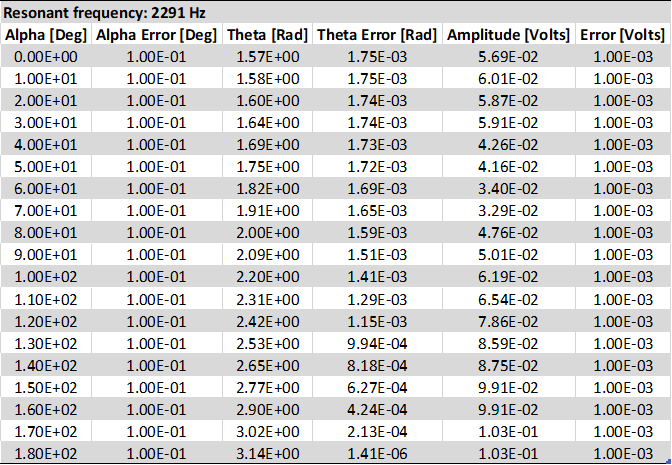
\includegraphics[width=0.45\textwidth]{Tables/2291Table.png}
		\caption{Data table for resonant frequency $2291$ Hz.}
		\label{2291Table}		
	\end{table} 
	\columnbreak
	\begin{figure}[H]
		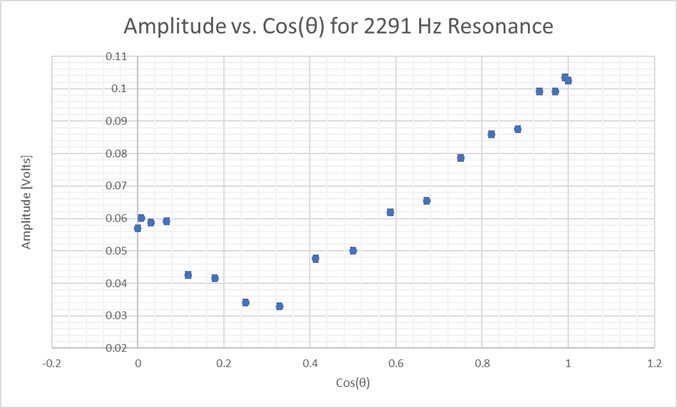
\includegraphics[width=0.45\textwidth]{Graphs/2291Graph.png}
		\caption{Graph of \cref{2291Table}. We can clearly see a single node at $\theta = 1.91$ radians.}
		\label{2291Graph}
	\end{figure}
\end{multicols}

\pagebreak

\begin{multicols}{2}
	\begin{table}[H]
		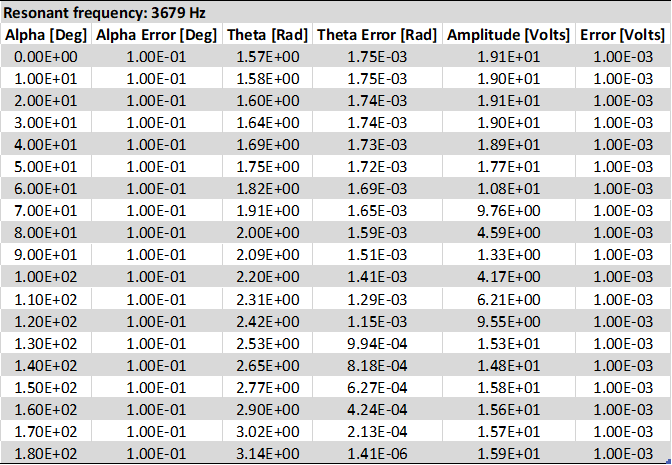
\includegraphics[width=0.45\textwidth]{Tables/3679Table.png}
		\caption{Table showing amplitude vs polar angle for 3679 Hz resonance.}
		\label{3679Table}		
	\end{table} 
	\columnbreak
	\begin{figure}[H]
		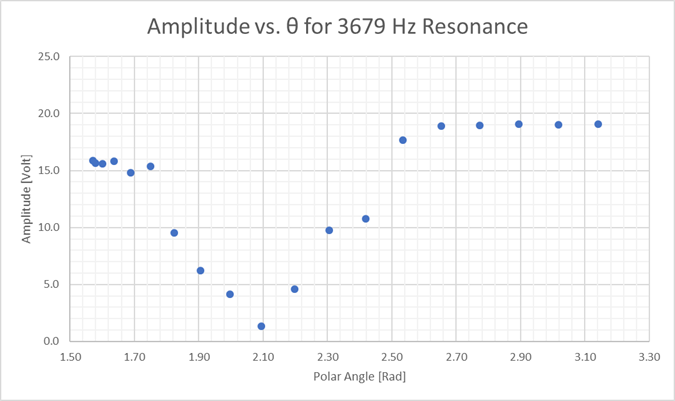
\includegraphics[width=0.45\textwidth]{Graphs/3679Graph.png}
		\caption{Graph of \cref{3679Table}. We can clearly see a single node at $\theta = 2.09$ radians.}
		\label{3679Graph}
	\end{figure}
\end{multicols}



\begin{multicols}{2}	
	\begin{table}[H]
		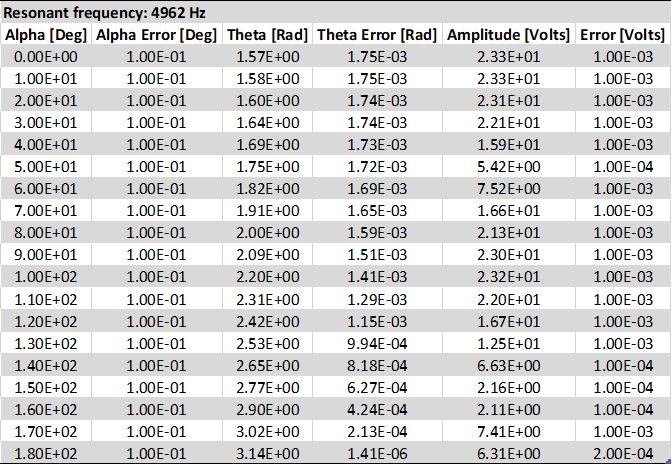
\includegraphics[width=0.45\textwidth]{Tables/4962Table.png}
		\caption{Table showing amplitude vs polar angle for 4926 Hz resonance.}
		\label{4962Table}		
	\end{table}
	\columnbreak
	\begin{figure}[H]
		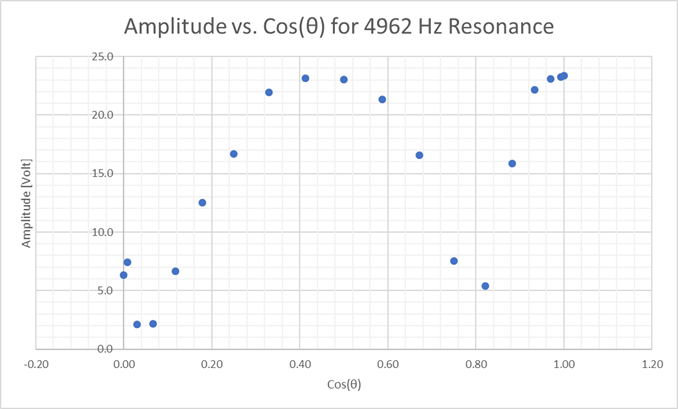
\includegraphics[width=0.45\textwidth]{Graphs/4962Graph.png}
		\caption{Graph of \cref{4962Table}. We can clearly see a single node at $\theta = $ radians.}
		\label{4962Graph}
	\end{figure}
\end{multicols}


\begin{multicols}{2}	
	\begin{table}[H]
		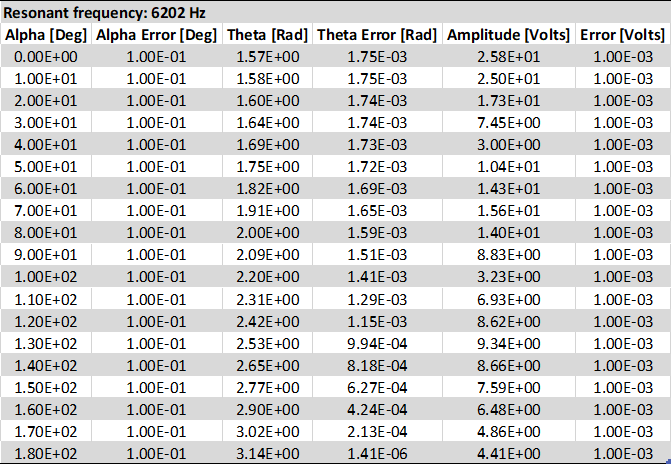
\includegraphics[width=0.45\textwidth]{Tables/6202Table.png}
		\caption{Table showing amplitude vs polar angle for 6202 Hz resonance.}
		\label{6202Table}		
	\end{table}
	\columnbreak
	\begin{figure}[H]
		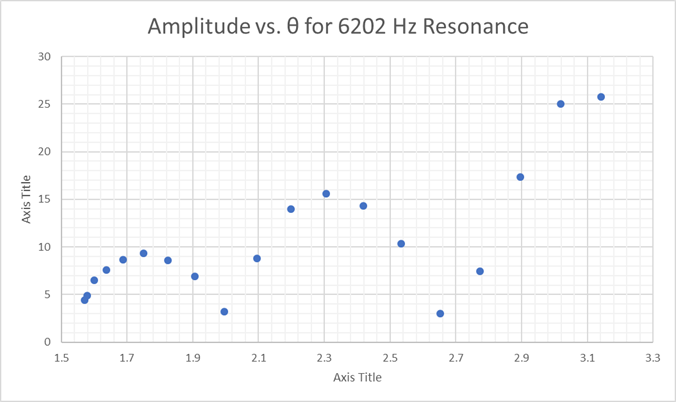
\includegraphics[width=0.45\textwidth]{Graphs/6202Graph.png}
		\caption{Graph of \cref{6202Table}. We can clearly see a single node at $\theta = $ radians.}
		\label{6202Graph}
	\end{figure}
\end{multicols}

\pagebreak

\begin{multicols}{2}	
	\begin{table}[H]
		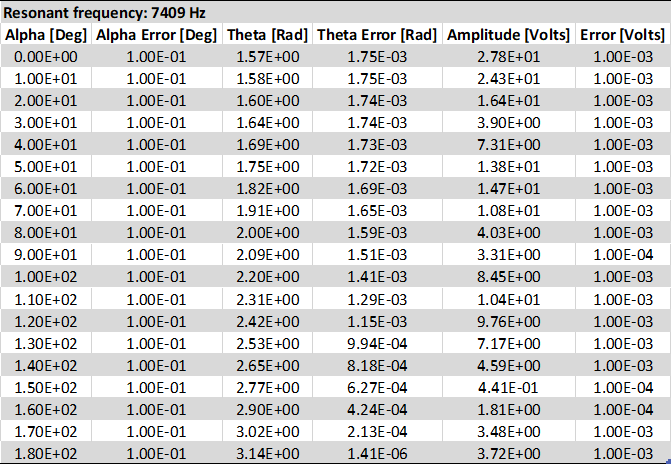
\includegraphics[width=0.45\textwidth]{Tables/7409Table.png}
		\caption{Table showing amplitude vs polar angle for 7409 Hz resonance.}
		\label{7409Table}		
	\end{table}
	\columnbreak
	\begin{figure}[H]
		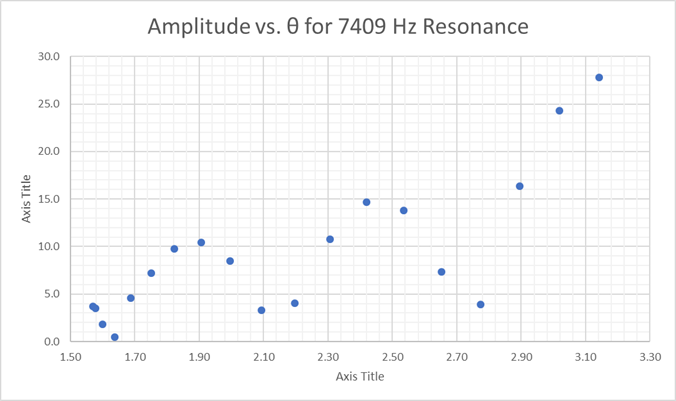
\includegraphics[width=0.45\textwidth]{Graphs/7409Graph.png}
		\caption{Graph of \cref{7409Table}. We can clearly see a single node at $\theta = $ radians.}
		\label{7409Graph}
	\end{figure}
\end{multicols}


\subsection{Legender Polynomial Comparisons}
\begin{figure}[H]
	\centering
	\subfloat[Measured acoustic amplitude plotted against $\cos(\theta)$ for the 2291 Hz resonance]{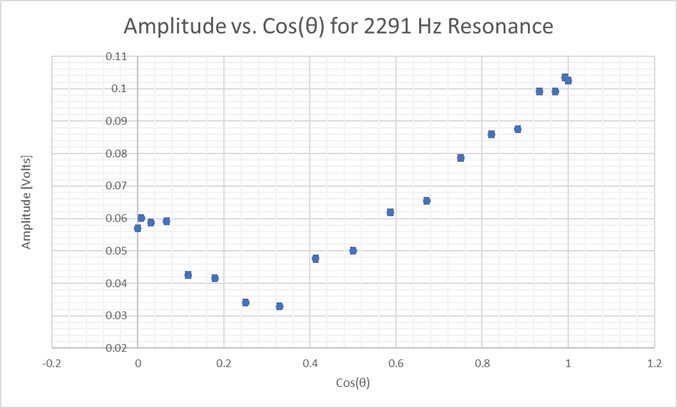
\includegraphics[height=6cm]{Graphs/2291Graph.png}}
	\qquad
	\subfloat[Legendre polynomial $|\mathrm{P}_1|^2$]{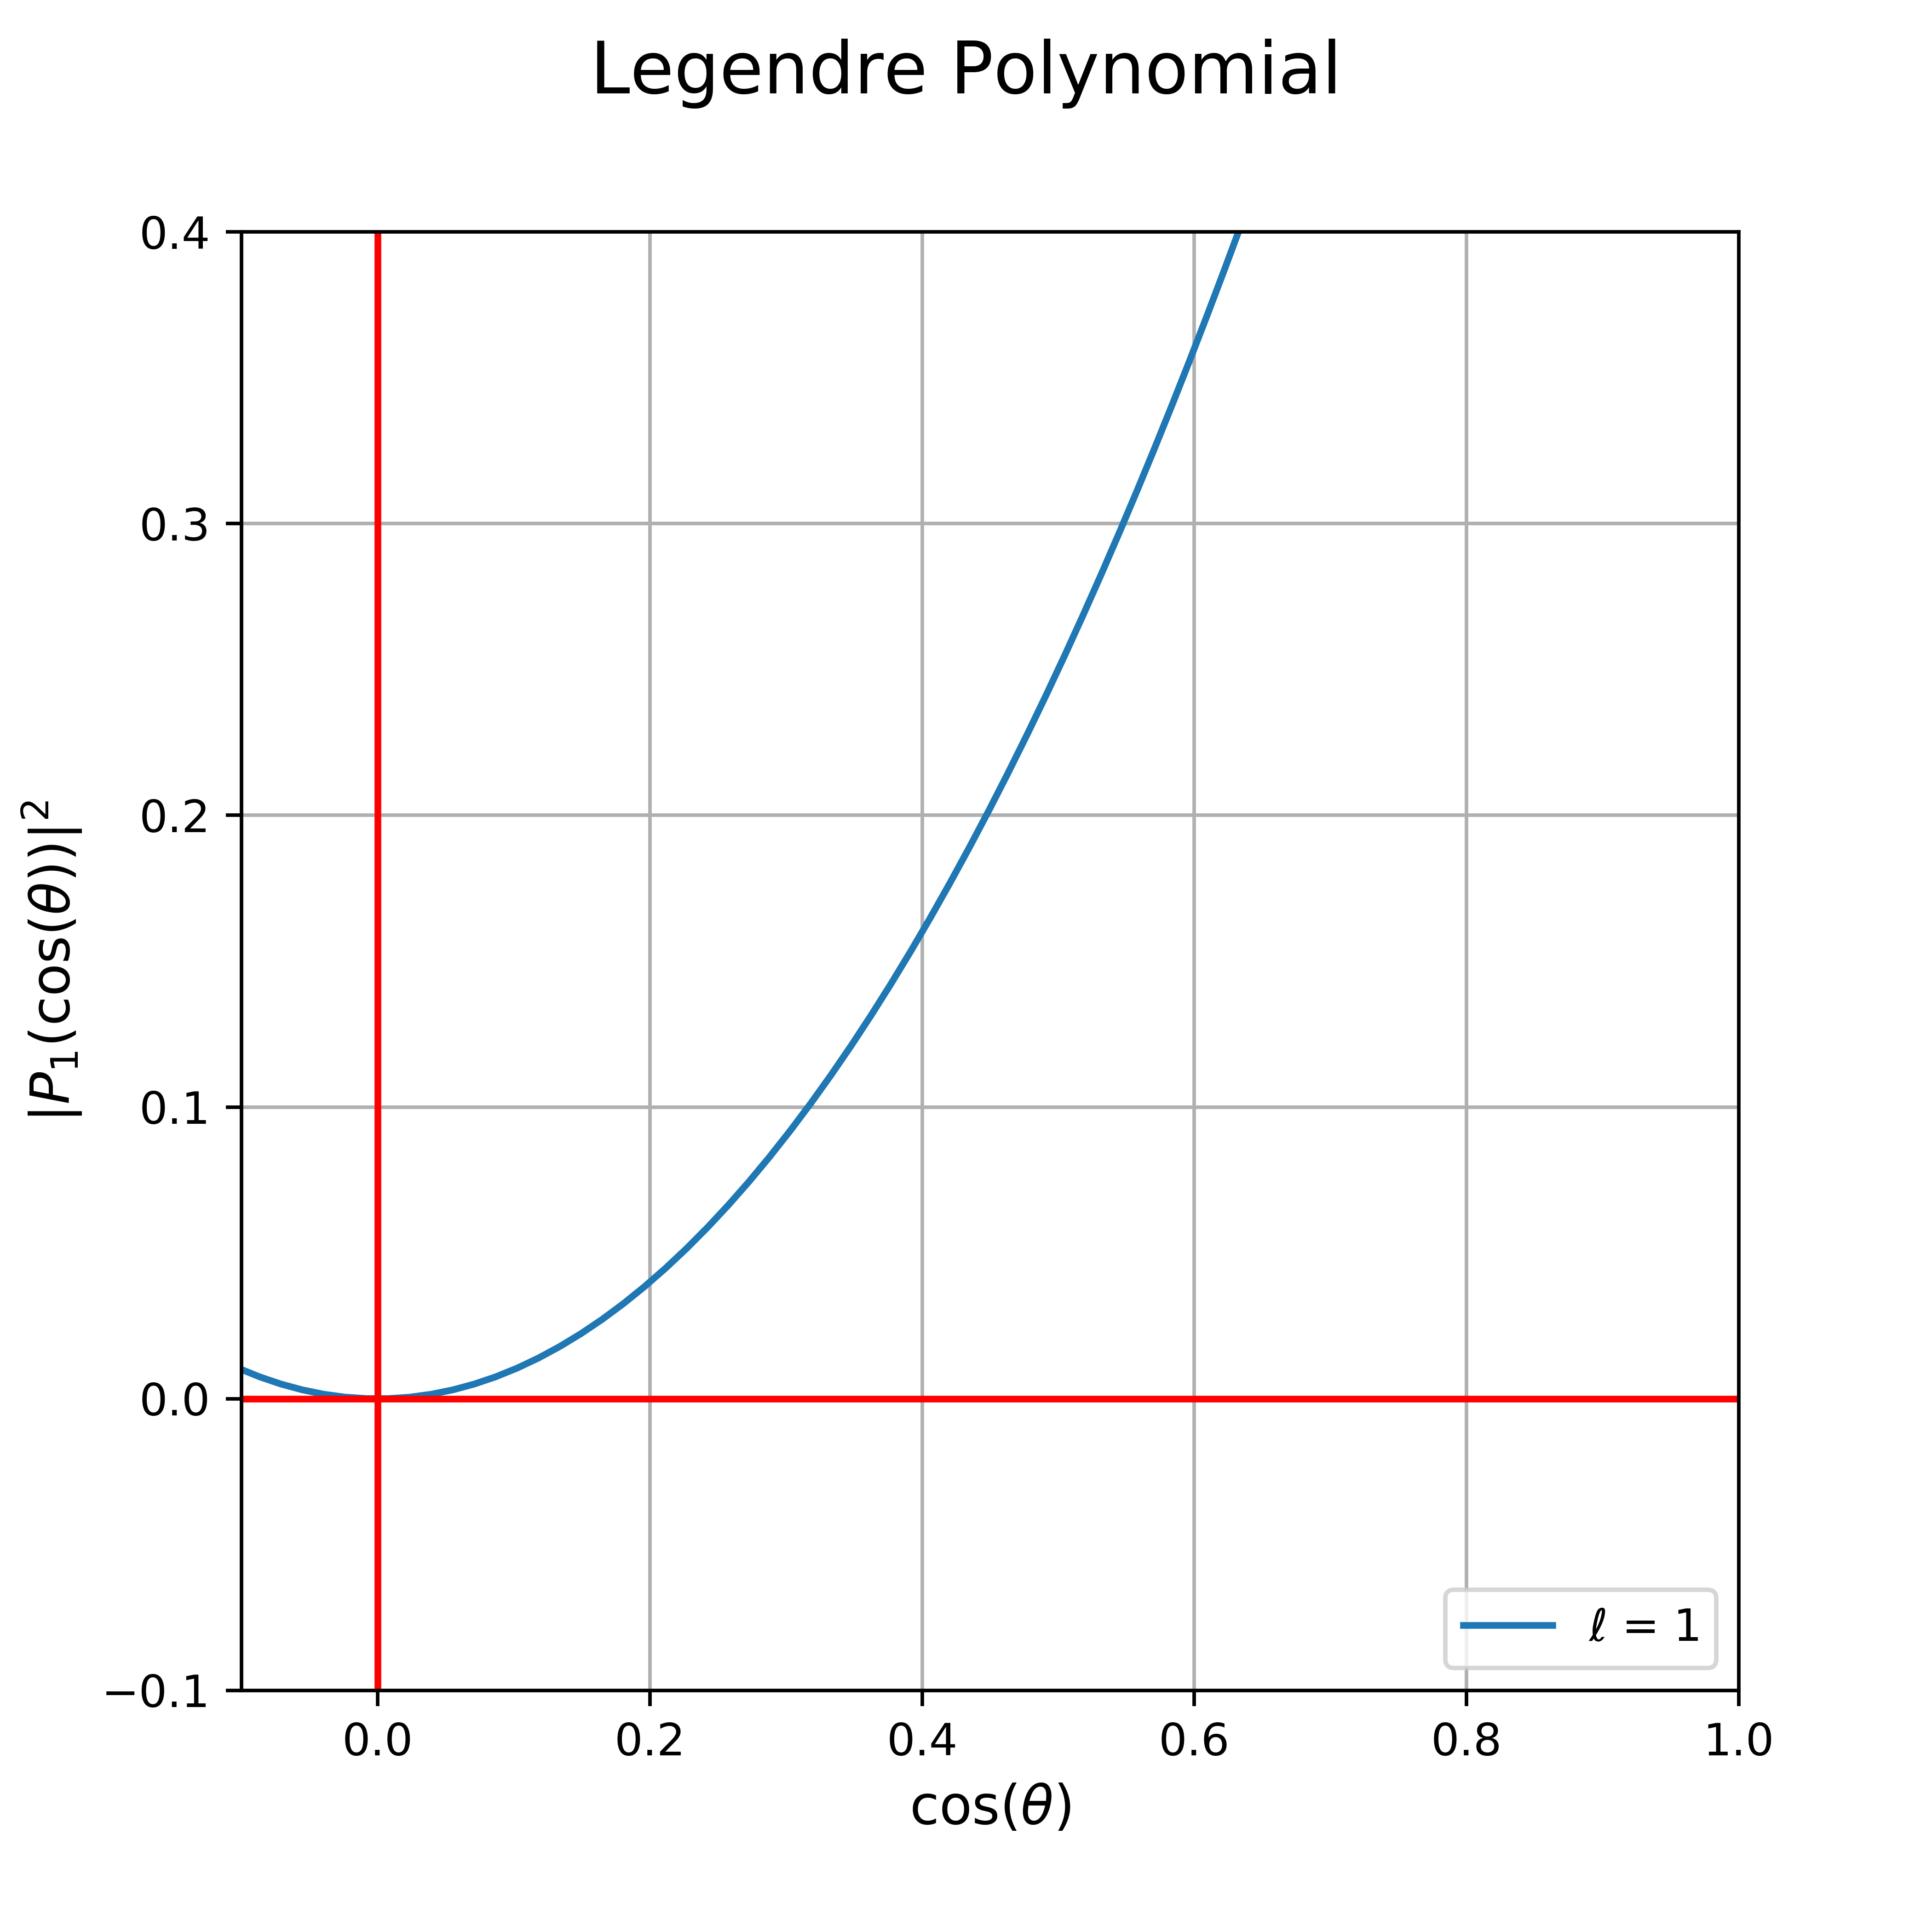
\includegraphics[height=6cm]{Legendre/legendreL1.png}\label{L1}}
	\caption{Comparison of the measured data and the $\ell=1$ Legendre polynomial for the $2291$ Hz resonance.}
	\label{legendre1}
\end{figure}

\begin{figure}[H]
	\centering
	\subfloat[Measured acoustic amplitude plotted against $\cos(\theta)$ for the 3679 Hz resonance]{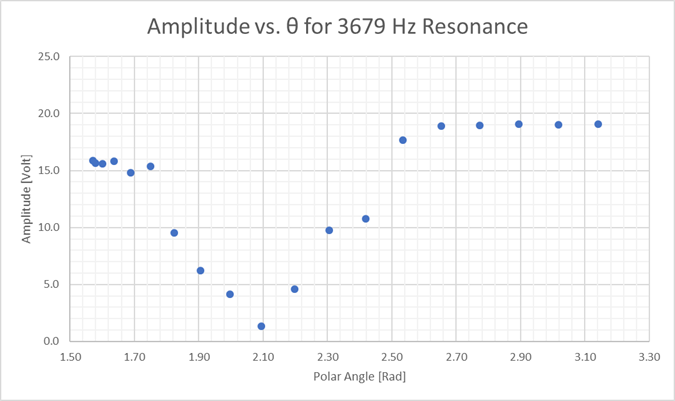
\includegraphics[height=6cm]{Graphs/3679Graph.png}}
	\qquad
	\subfloat[Legendre polynomial $|\mathrm{P}_2|^2$]{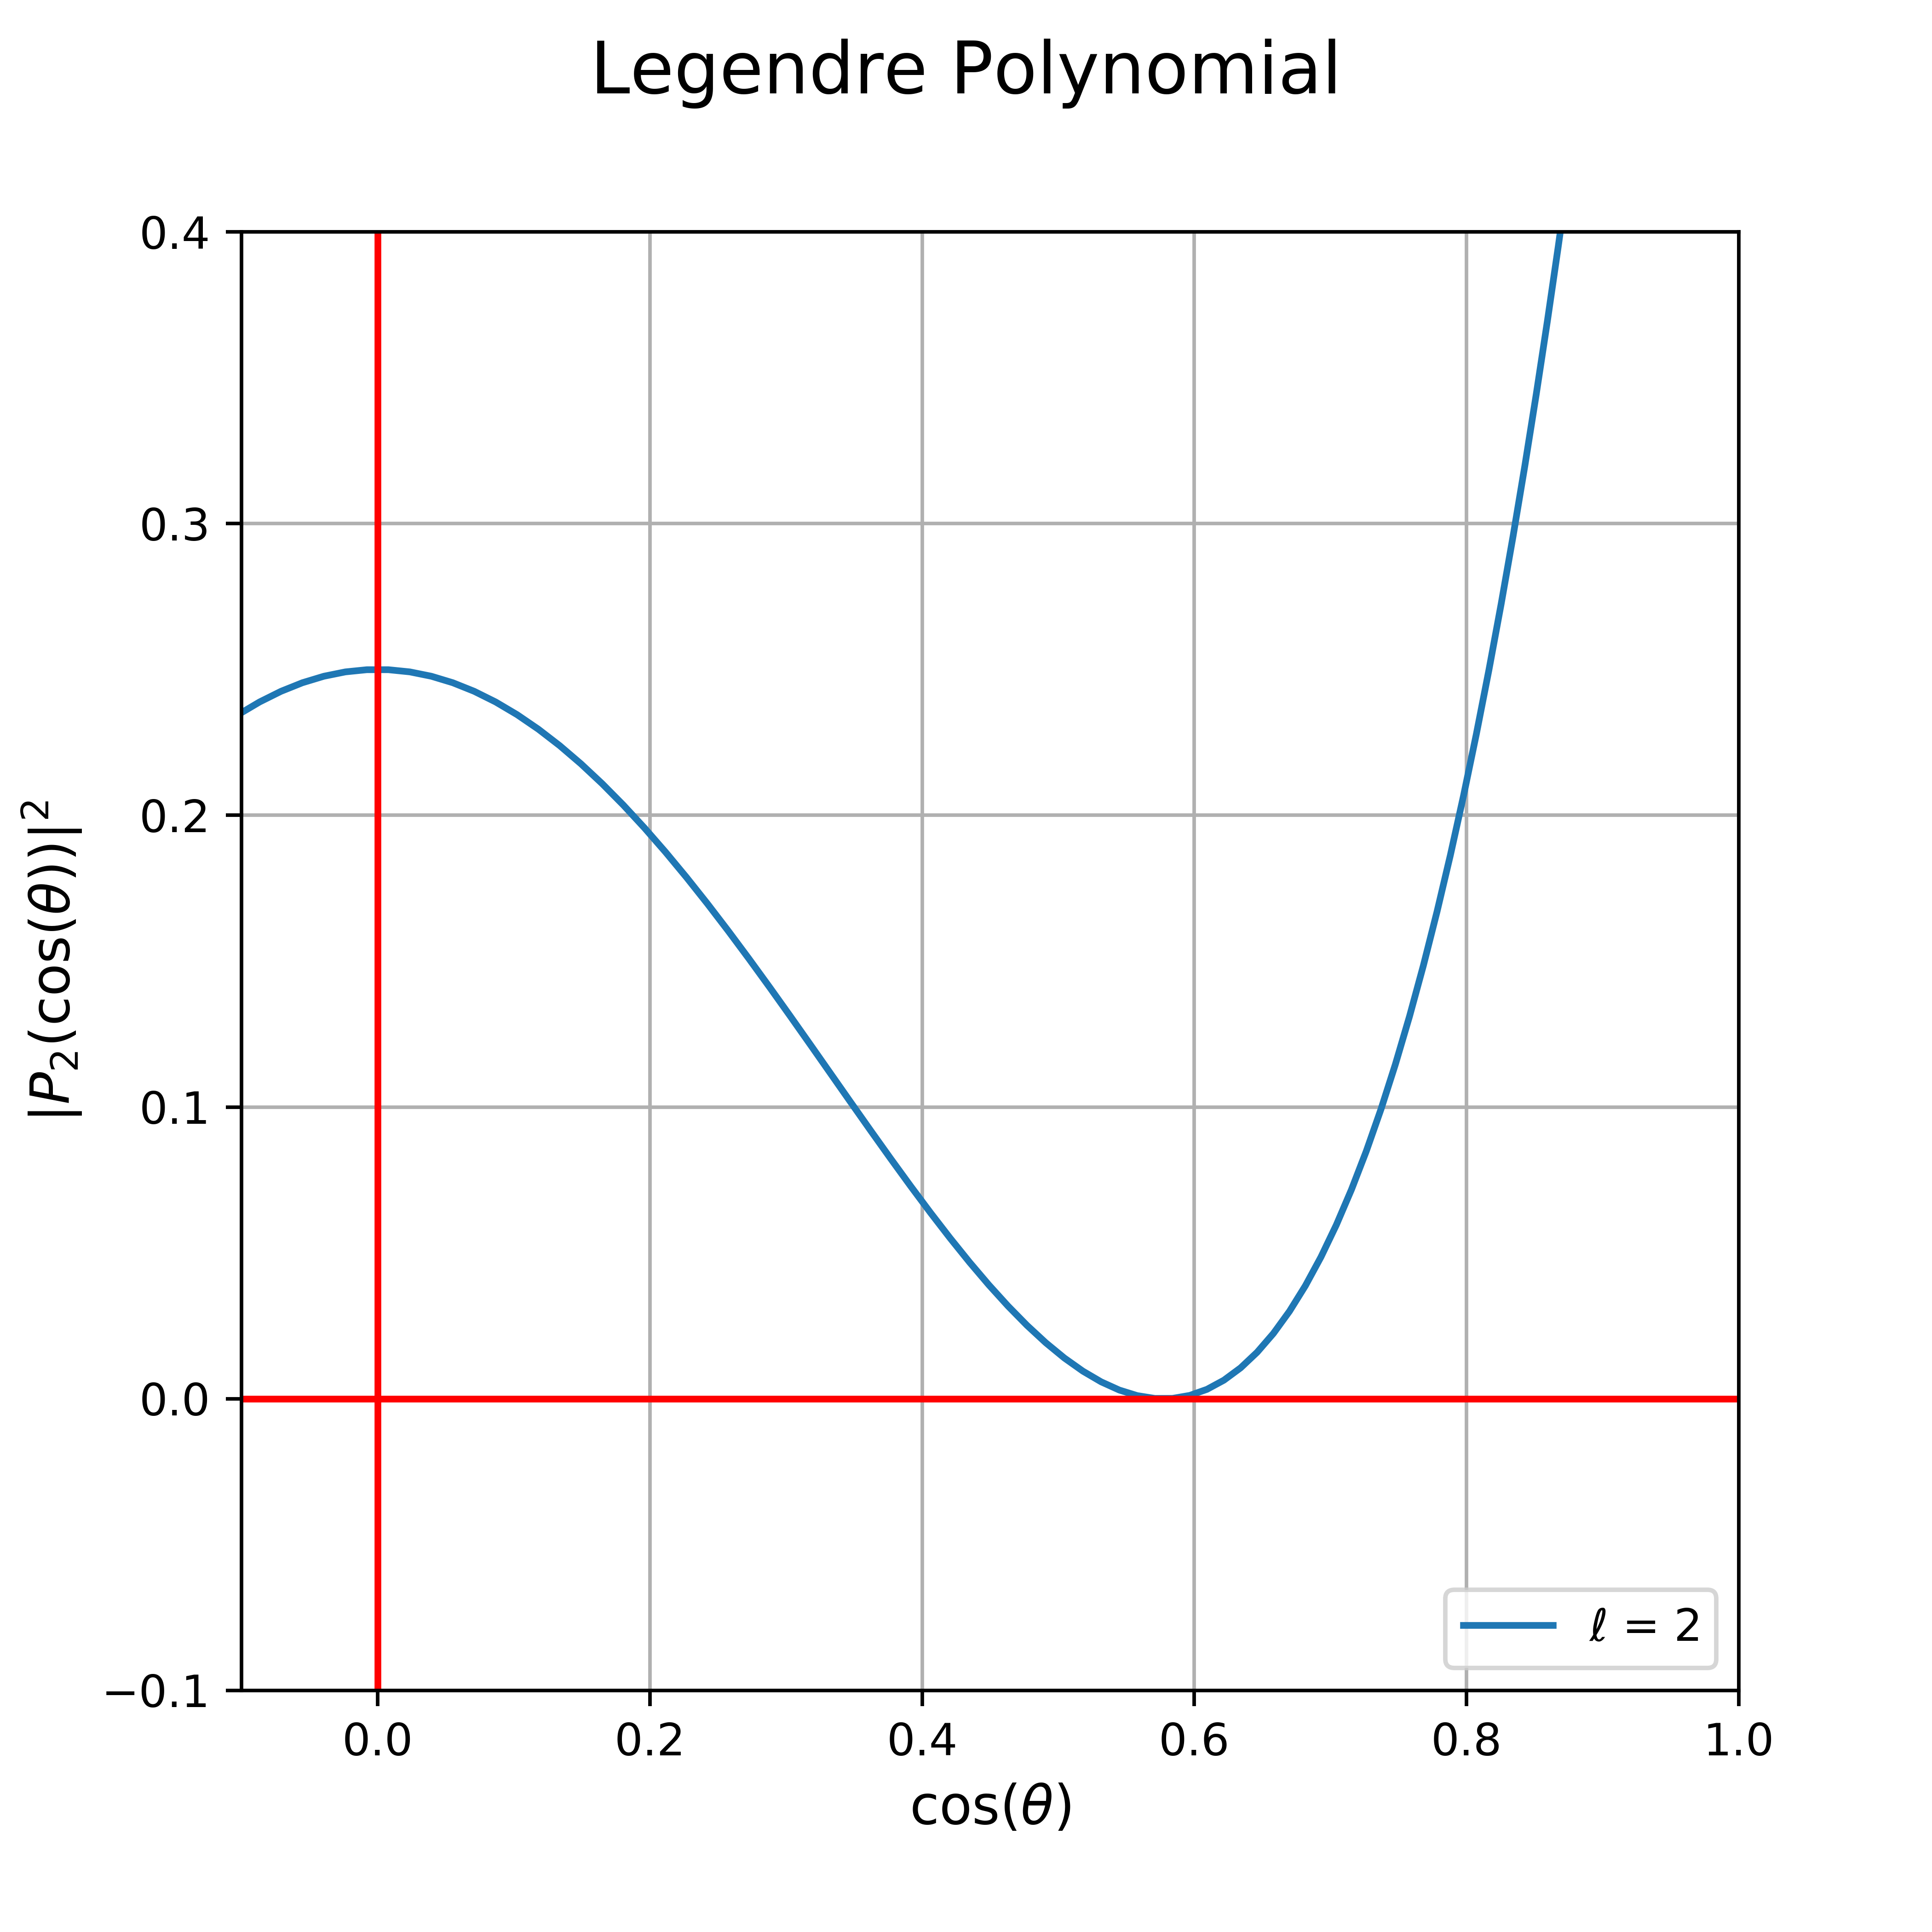
\includegraphics[height=6cm]{Legendre/legendreL2.png}\label{L2}}
	\caption{Comparison of the measured data and the $\ell=2$ Legendre polynomial for the $3679$ Hz resonance.}
	\label{legendre2}
\end{figure}

\begin{figure}[H]
	\centering
	\subfloat[Measured acoustic amplitude plotted against $\cos(\theta)$ for the 4962 Hz resonance]{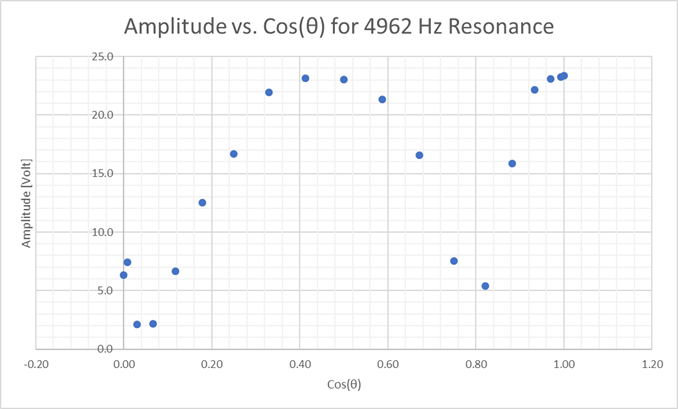
\includegraphics[height=6cm]{Graphs/4962Graph.png}}
	\qquad
	\subfloat[Legendre polynomial $|\mathrm{P}_3|^2$]{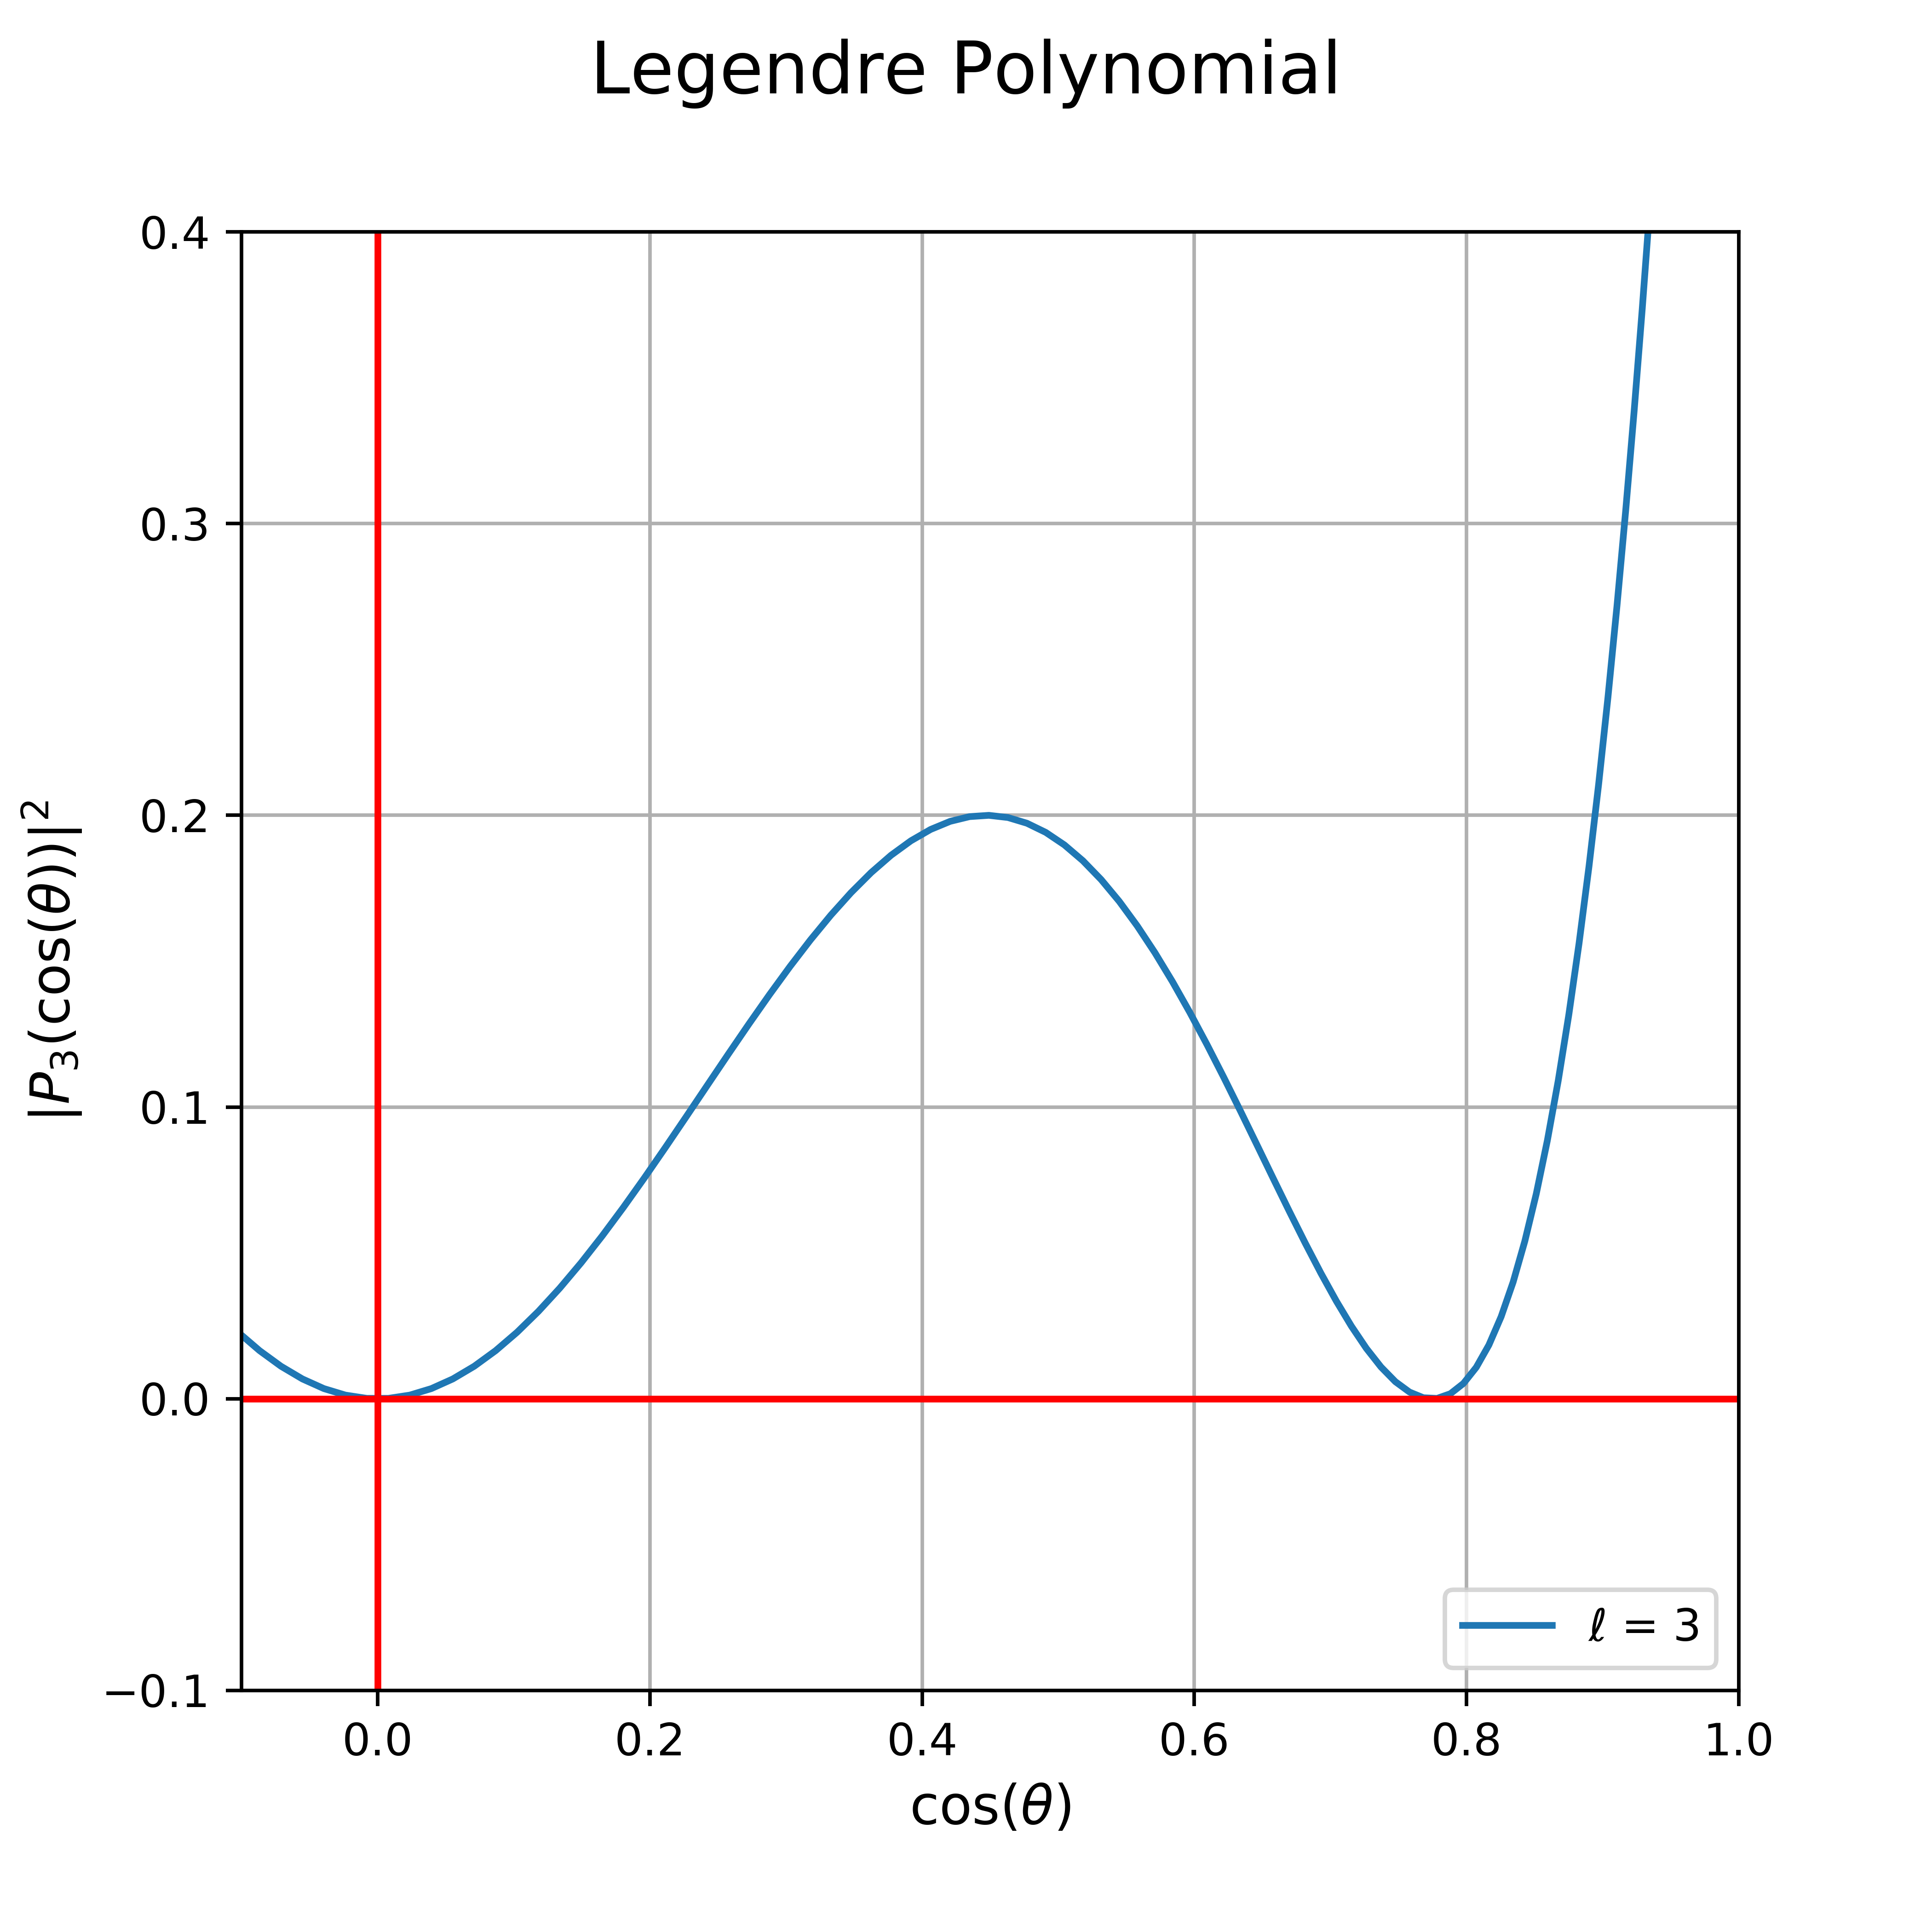
\includegraphics[height=6cm]{Legendre/legendreL3.png}\label{L3}}
	\caption{Comparison of the measured data and the $\ell=3$ Legendre polynomial for the $4962$ Hz resonance.}
	\label{legendre3}
\end{figure}

\begin{figure}[H]
	\centering
	\subfloat[Measured acoustic amplitude plotted against $\cos(\theta)$ for the 6202 Hz resonance]{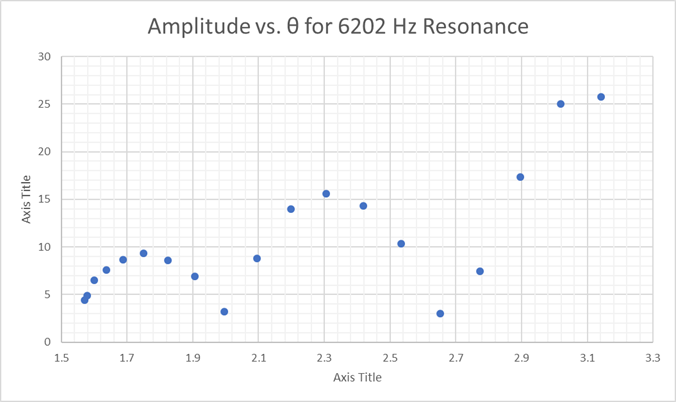
\includegraphics[height=6cm]{Graphs/6202Graph.png}}
	\qquad
	\subfloat[Legendre polynomial $|\mathrm{P}_4|^2$]{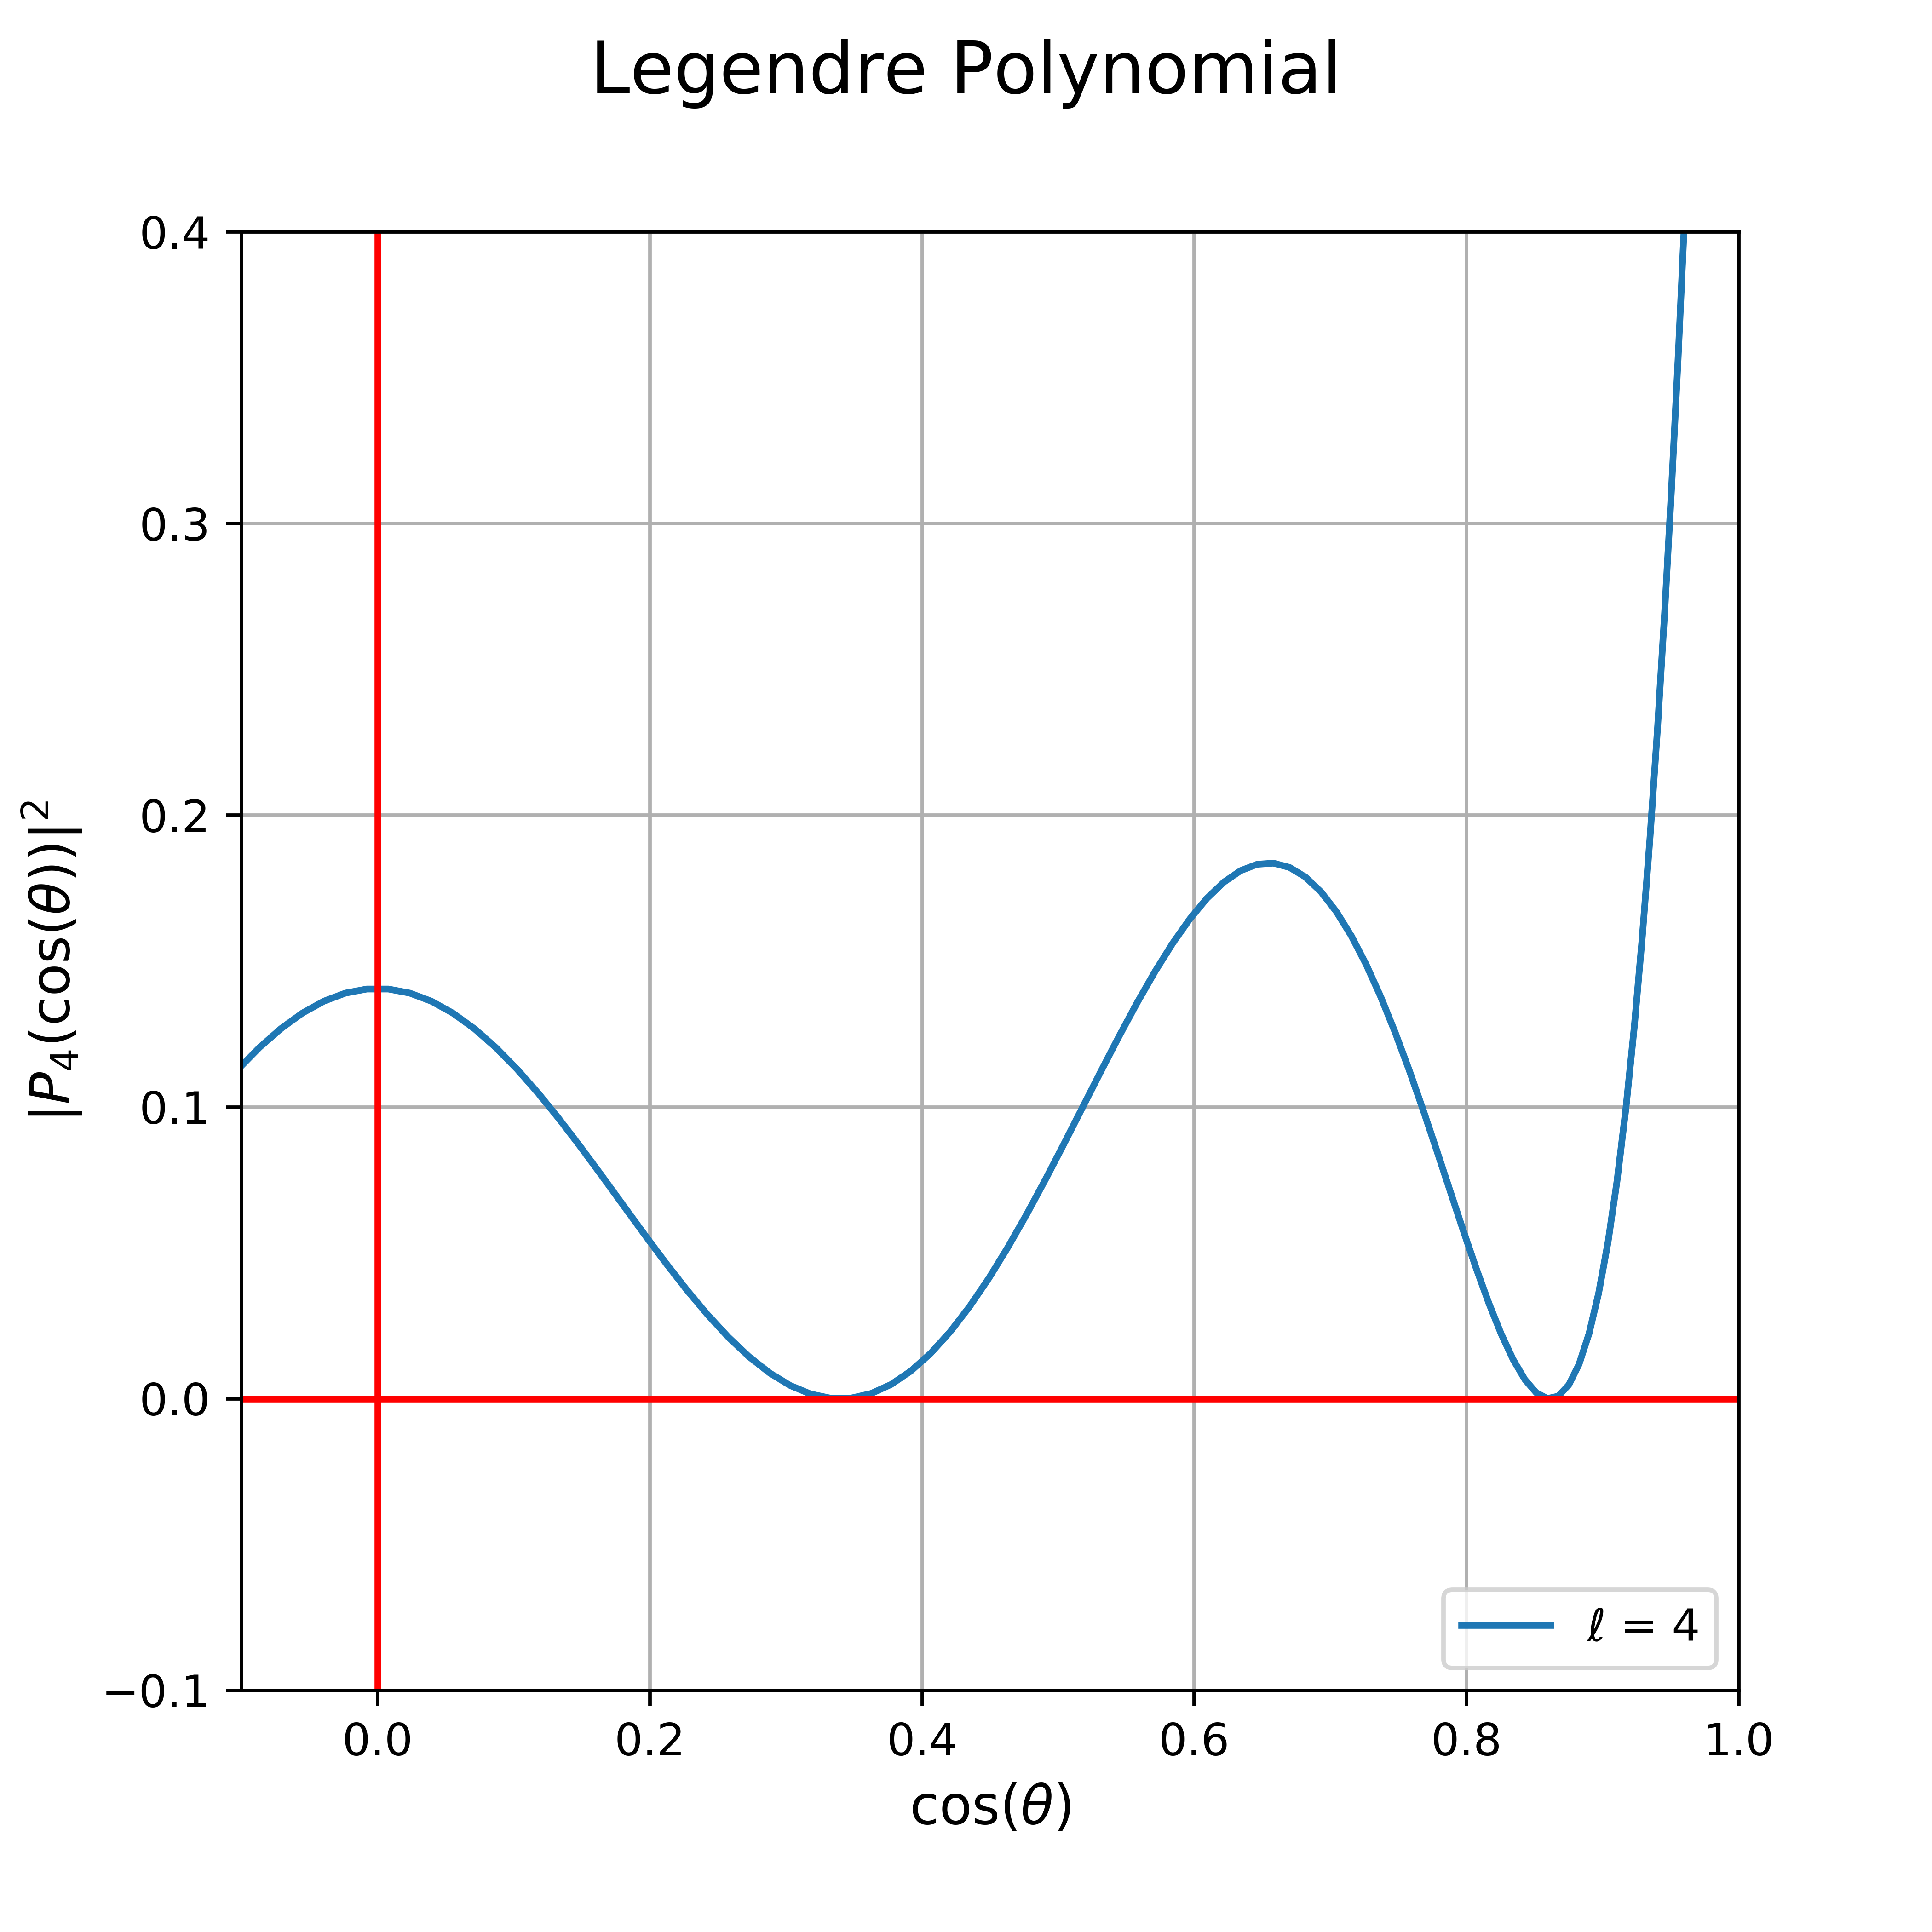
\includegraphics[height=6cm]{Legendre/legendreL4.png}\label{L4}}
	\caption{Comparison of the measured data and the $\ell=4$ Legendre polynomial for the $6202$ Hz resonance.}
	\label{legendre4}
\end{figure}

\begin{figure}[H]
	\centering
	\subfloat[Measured acoustic amplitude plotted against $\cos(\theta)$ for the 7409 Hz resonance]{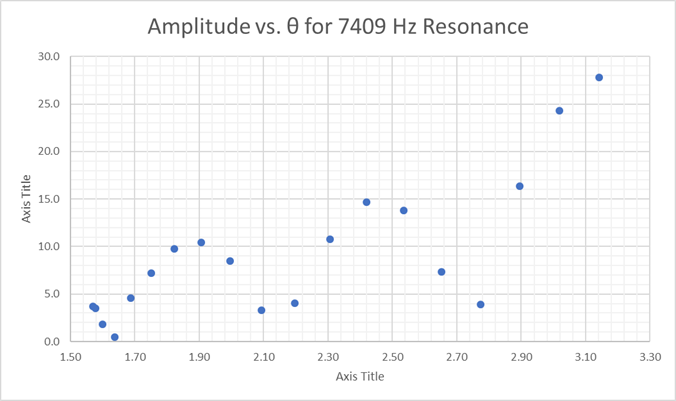
\includegraphics[height=6cm]{Graphs/7409Graph.png}}
	\qquad
	\subfloat[Legendre polynomial $|\mathrm{P}_5|^2$]{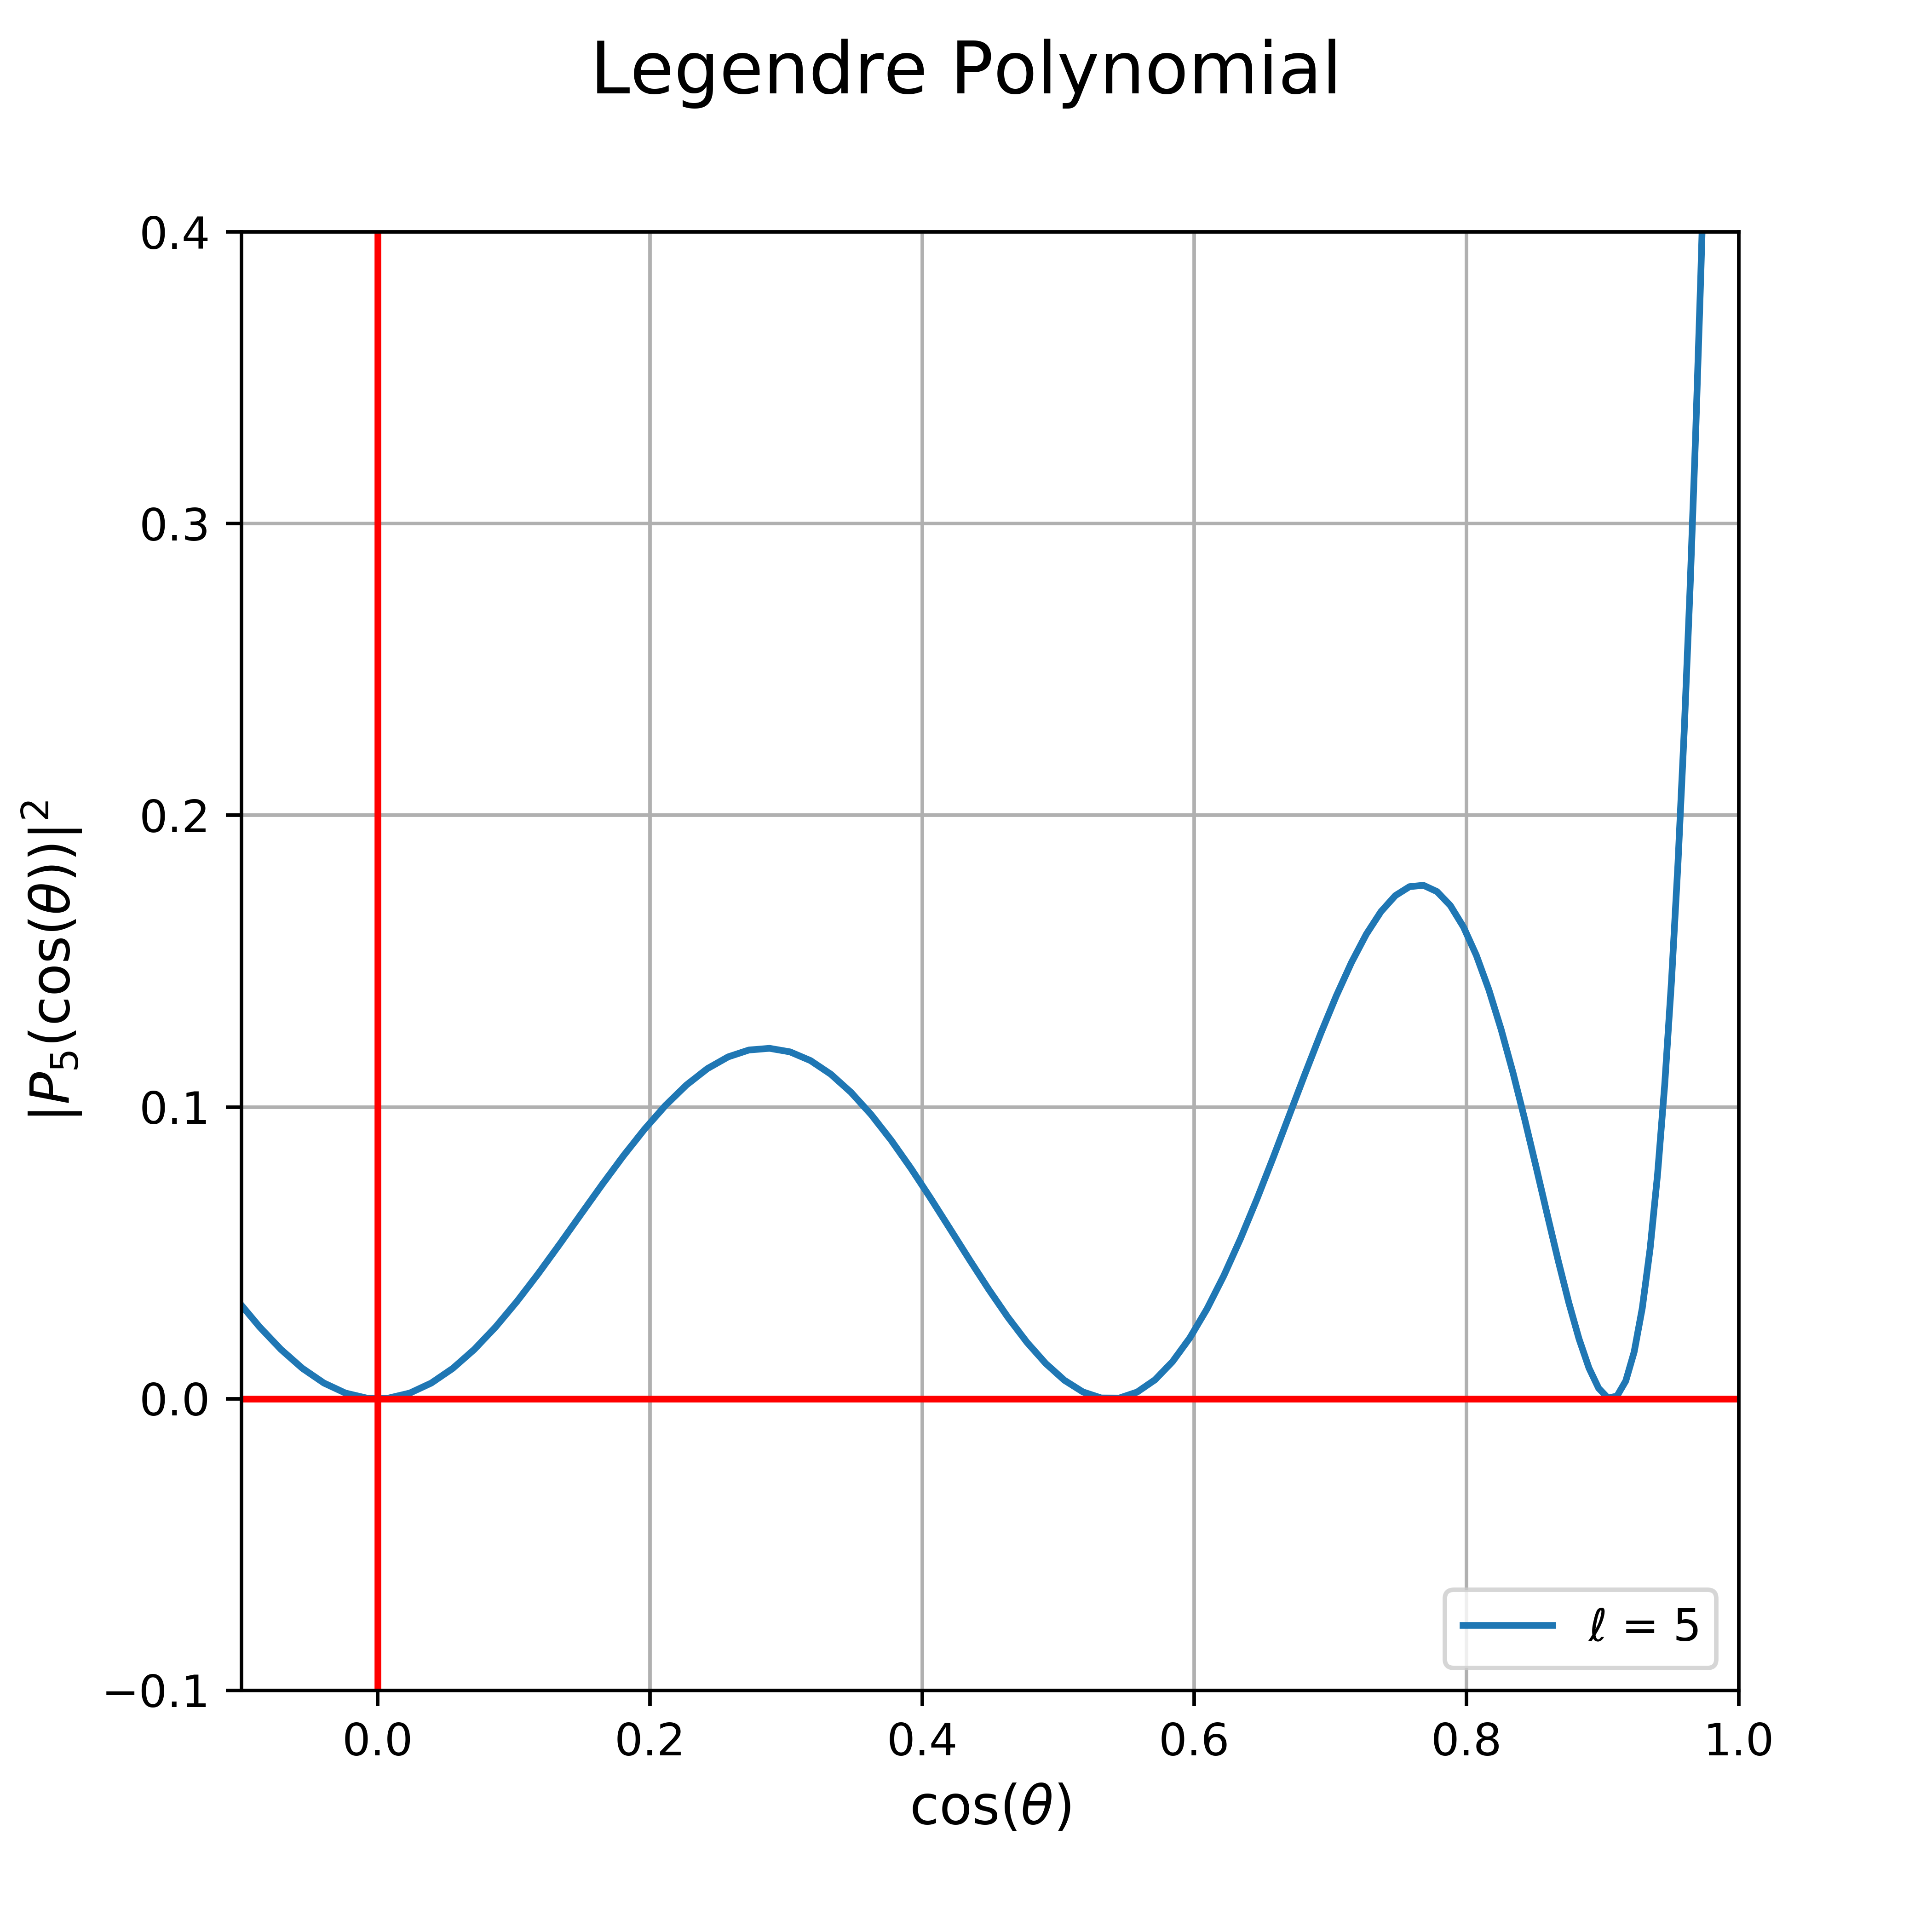
\includegraphics[height=6cm]{Legendre/legendreL5.png}\label{L5}}
	\caption{Comparison of the measured data and the $\ell=5$ Legendre polynomial for the $7409$ Hz resonance.}
	\label{legendre5}
\end{figure}

\subsection{Spherical Harmonics}


\begin{figure}[H]
	\centering
	\subfloat[$\ell=1$, $m=0$ polar plot for 2291 Hz resonance]{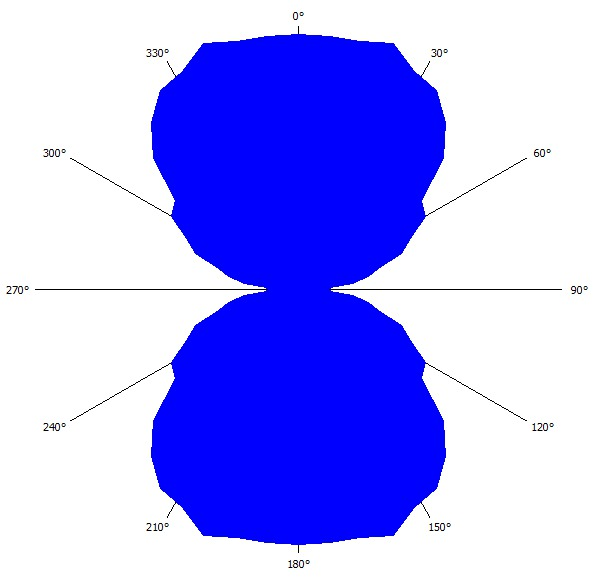
\includegraphics[width=0.35\textwidth]{2.3.2/F2291.jpg}\label{Polar2291}}
	\qquad \qquad
	\subfloat[$\ell=2$, $m=0$  plot for 3679 Hz resonance ]{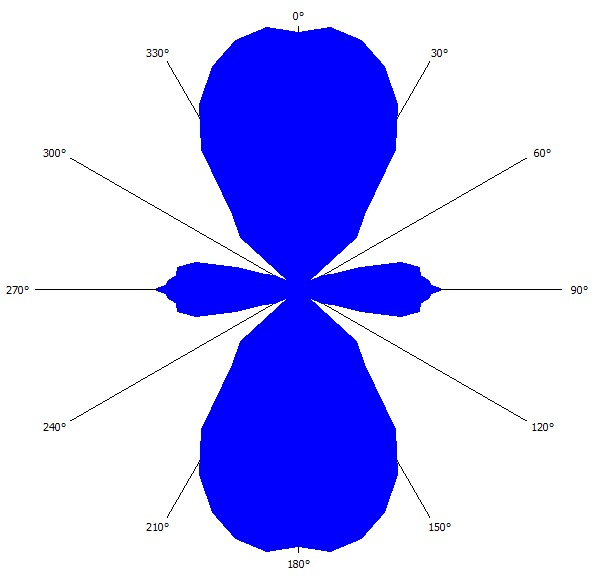
\includegraphics[width=0.35\textwidth]{2.3.2/F3679.jpg}\label{Polar3679}}
	\\
	\subfloat[$\ell=3$, $m=0$  plot for 4962 Hz resonance]{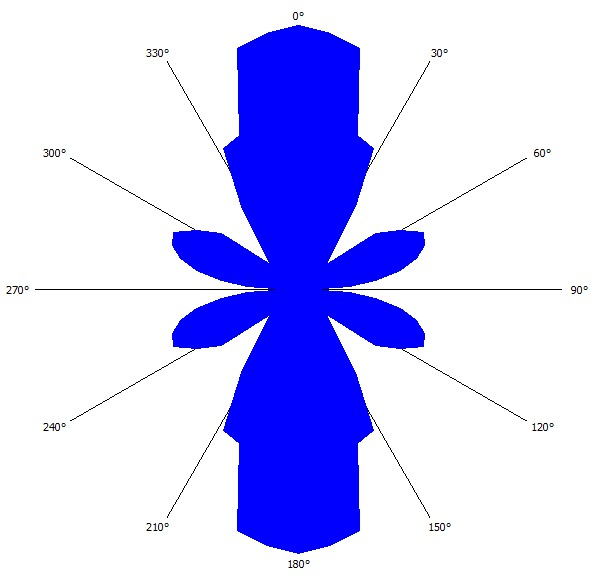
\includegraphics[width=0.35\textwidth]{2.3.2/F4962.jpg}\label{Polar4962}}
	\qquad \qquad
	\subfloat[$\ell=5$, $m=0$  plot for 7409 Hz resonance]{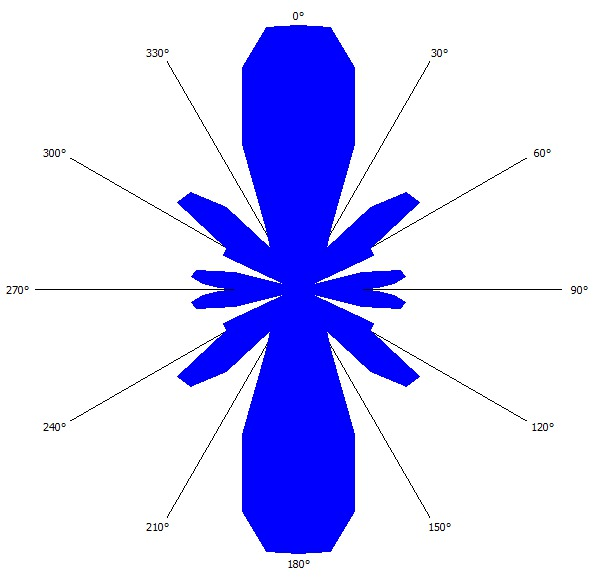
\includegraphics[width=0.35\textwidth]{2.3.2/F7409.jpg}\label{Polar6202}}
	\caption{Acoustic amplitude vs polar angle ($\theta$) with azimuthal angle $\varphi = 0$ for 4 resonant frequencies. Comparing these to the spherical harmonics in \cref{sphereHarm}, it is possible to determine the angular momentum quantum number $\ell$ for each resonance.}
	\label{polarGraphs}
\end{figure}

\begin{figure}[H]
	\centering
	\subfloat[Spherical harmonic for $\ell = 1$, $m= 0$]{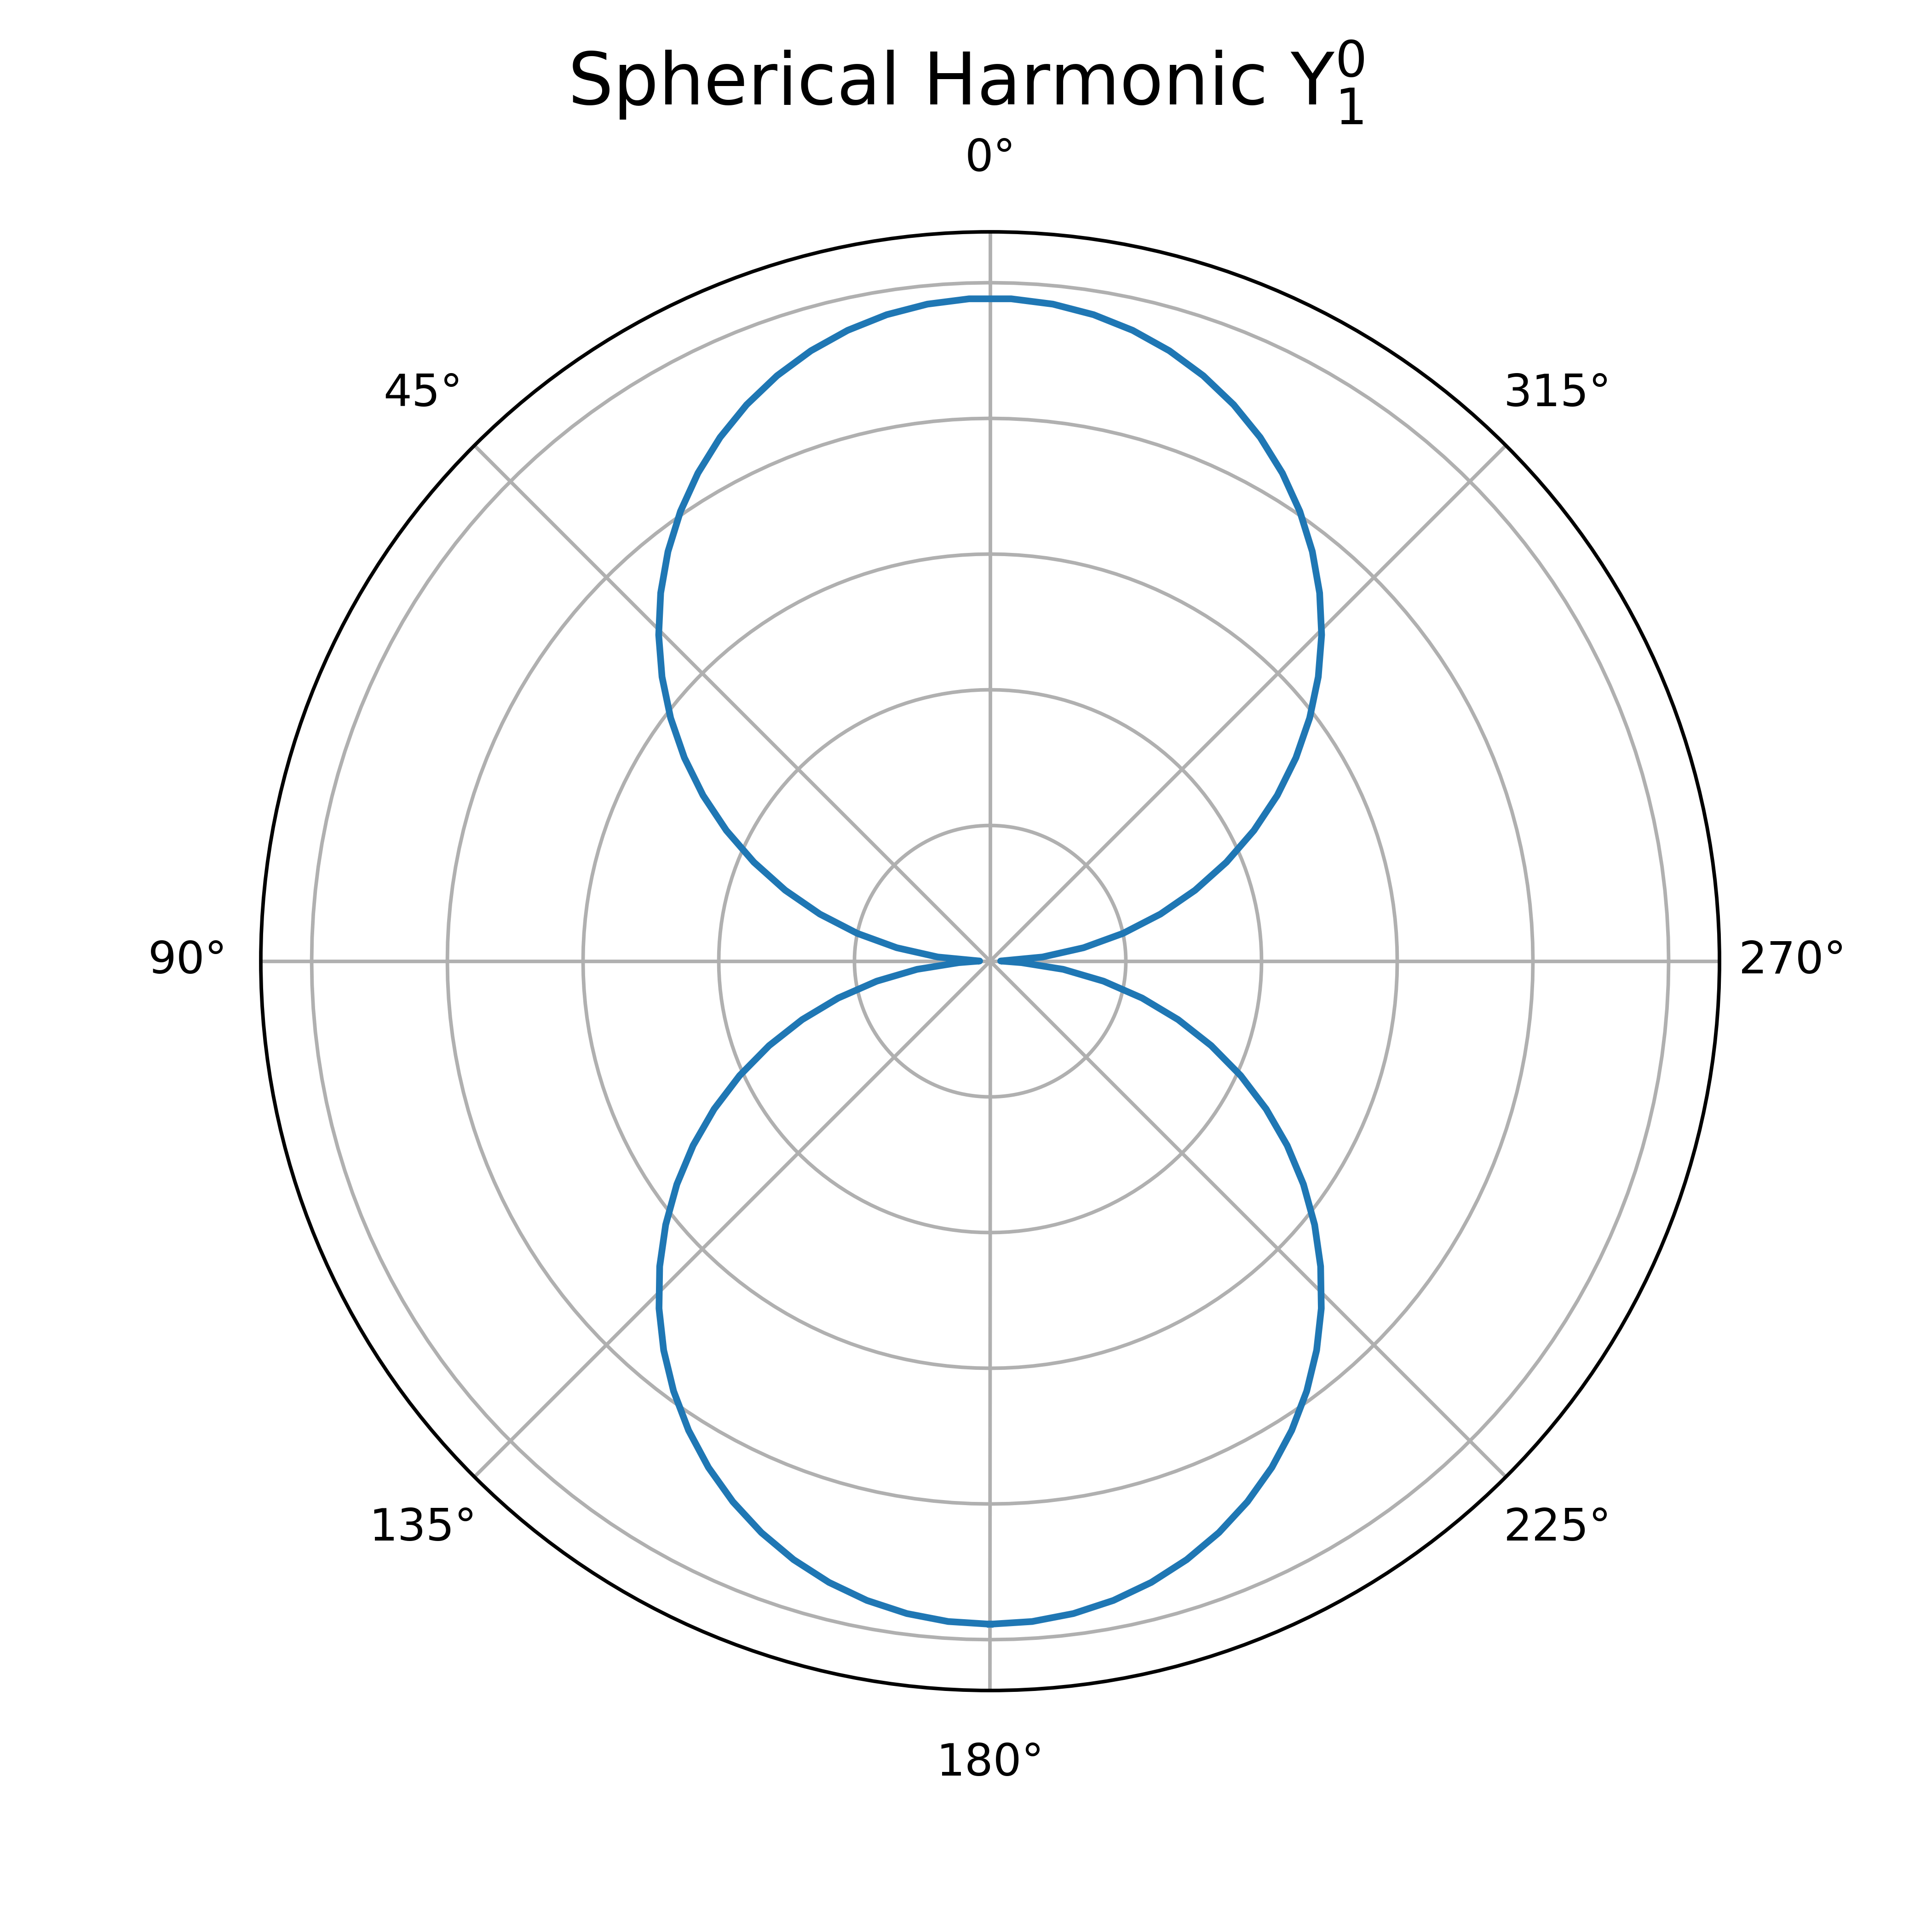
\includegraphics[width=0.4\textwidth]{SphHarm/SphHarmL1M0.png}\label{sphHarmL1M0}}
	\qquad \quad
	\subfloat[Spherical harmonic for $\ell = 2$, $m=0$]{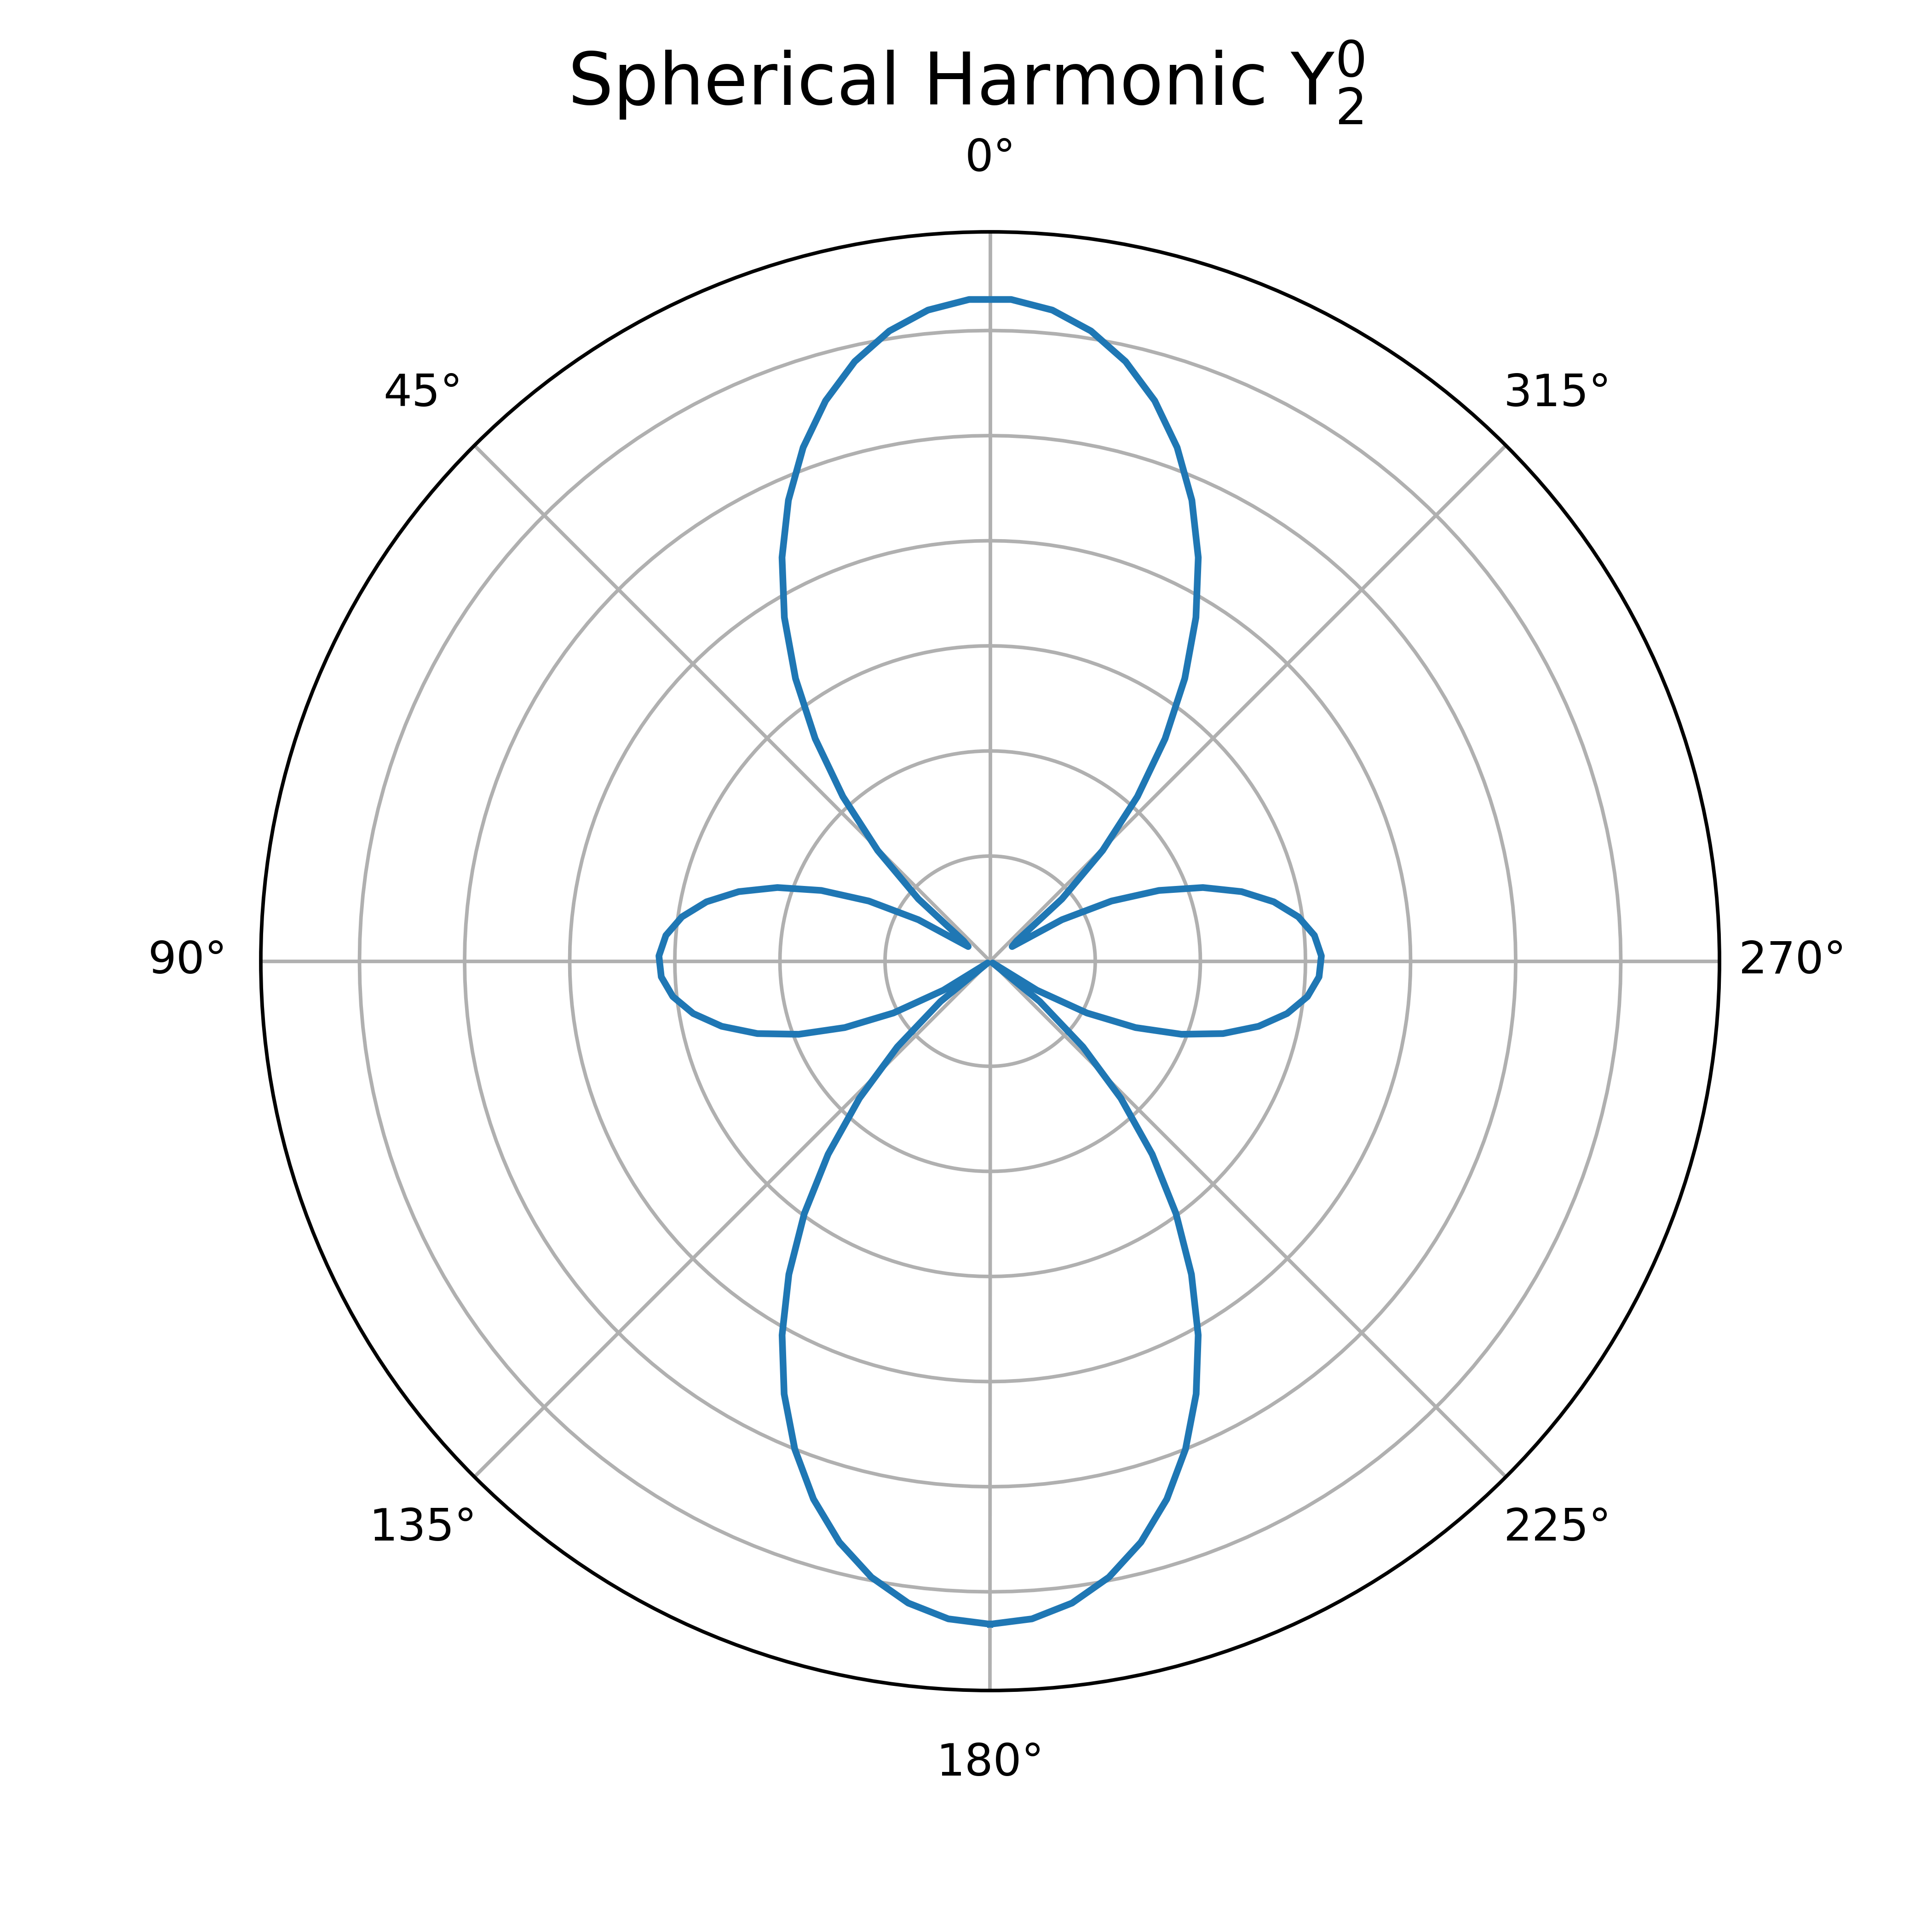
\includegraphics[width=0.4\textwidth]{SphHarm/SphHarmL2M0.png}\label{sphHarmL2M0}}
	\\
	\subfloat[Spherical harmonic for $\ell = 3$, $m = 0$]{\includegraphics[width=0.4\textwidth]{SphHarm/SphHarmL3M0.png}\label{sphHarmL3M0}}
	\qquad \quad
	\subfloat[Spherical harmonic for $\ell = 5$, $m = 1$]{\includegraphics[width=0.4\textwidth]{SphHarm/SphHarmL5M0.png}\label{sphHarmL5M0}}
	\caption{Projections of the spherical harmonics $\mathrm{Y}^\ell_m$ onto the $\varphi = 0$ plane. Angle markings indicate polar angle $\theta$.}
	\label{sphereHarm}
\end{figure}

\subsection{Polar Graphs with Broken Cavity Symmetry}


\begin{figure}[H]
	\captionsetup{justification = centering}
	\centering
	\subfloat[$\ell=1$, $m=0$]{\includegraphics[width=0.35\textwidth]{Day4/L13mmPolar2084_806.png}}
	\qquad \quad
	\subfloat[$\ell=1$, $m=\pm1$]{\includegraphics[width=0.35\textwidth]{Day4/L13mmPolar2251_140.png}}
	\caption{Amplitude versus polar angle $\theta$ for the $\ell=1$ resonance with 3mm Spacing}
	\label{3mmliftedDegeneracy}
\end{figure}


\begin{figure}[H]
	\captionsetup{justification = centering}
	\centering
	\subfloat[[$\ell=1$, $m=0$]{\includegraphics[width=0.35\textwidth]{Day4/L16mmPolar2084_806.png}}
	\qquad \quad
	\subfloat[[$\ell=1$, $m=\pm1$]{\includegraphics[width=0.35\textwidth]{Day4/L16mmPolar2251_140.png}}
	\caption{Amplitude versus polar angle $\theta$ for the $\ell=1$ resonance with 6mm Spacing}
	\label{6mmliftedDegeneracy}
\end{figure}

We can see that as the cavity separation is increased, simulating a stronger magnetic field, the shapes of the orbitals becomes more symmetric.


%	\begin{figure}[H]
%		\centering
%		\subfloat[$\ell=2$, $m=-1$ resonance]{\includegraphics[width=0.3\textwidth]{2.3.3/3mmPolar/323_Polar_L1M-1Amp_freq3591_549.png} \label{3-0mmDegeneracy}}
%		\quad
%		\subfloat[$\ell=2$, $m=0$ resonance]{\includegraphics[width=0.3\textwidth]{2.3.3/3mmPolar/323_Polar_L1M1Amp_freq3647_513.png} \label{3-1mmDegeneracy}}
%		\caption{Polar plots of lifted degeneracies for 3mm spacing}
%		\label{3mmliftedDegeneracy}
%	\end{figure}
%	It is important to note that not all the degeneracies were lifted at $3$ mm spacing.


%
%	\begin{figure}[H]
%		\centering
%		\subfloat[$\ell=1$, $m=-1$ resonance]{\includegraphics[width=0.3\textwidth]{2.3.3/6mmPolar/323_Polar_L1M-1Amp_freq3519_864.png} \label{6-m1mmDegeneracy}}
%		\quad
%		\subfloat[$\ell=1$, $m=0$ resonance]{\includegraphics[width=0.3\textwidth]{2.3.3/6mmPolar/323_Polar_L1M0Amp_freq3534_956.png} \label{6-0mmDegeneracy}}
%		\quad
%		\subfloat[$\ell=1$, $m=1$ resonance]{\includegraphics[width=0.3\textwidth]{2.3.3/6mmPolar/323_Polar_L1M1Amp_freq3632_422.png} \label{6-1mmDegeneracy}}
%		\caption{Polar plots of lifted degeneracies for 6mm spacing.}
%		\label{6mmliftedDegeneracy}
%	\end{figure}
%	
%	
%		Further, we focus on the \red{$\ell=2$} resonance and apply the spacing rings again to see how the peak splits.
%	
%	\begin{figure}[H]
%		\centering
%		\subfloat[Lifted degeneracy spectrum for $\ell=2$ 3mm spacing]{\includegraphics[width=0.3\textwidth]{2.3.3/323a180L13mmHires.png} \label{3mmDegeneracySpectrum}}
%		\quad
%		\subfloat[Lifted degeneracy spectrum for $\ell=2$ 6mm spacing]{\includegraphics[width=0.3\textwidth]{2.3.3/323a180L16mmHires.png} \label{6mmDegeneracySpectrum}}
%		\quad
%		\subfloat[Lifted degeneracy spectrum for $\ell=2$ 9mm spacing]{\includegraphics[width=0.3\textwidth]{2.3.3/323a180L19mmHires.png} \label{9mmDegeneracySpectrum}}
%		\caption{Progression of lifted degeneracies for the \red{$\ell=2$} state.}
%		\label{liftedDegeneracySpectrum}
%	\end{figure}

\newpage
\bibliographystyle{utphys}
\nocite{*} % Cite all things in the bibliography
\bibliography{references}


\end{document}